% ============= Package Einstellungen & Sonstiges ============= 
\documentclass[a4paper,12pt]{report}
\usepackage[left= 2.5 cm,right = 2.5 cm, bottom = 2.5 cm]{geometry}
\usepackage[onehalfspacing]{setspace}

\usepackage[
pdftitle={Studienarbeit},
pdfsubject={Entwicklung einer smarten Bewässerungslösung mit Web-Anbindung},
pdfauthor={Maximilian Schüller, Fynn Thierling, Justus Siegert, Lukas Maier, Timon Kleinknecht},
pdfkeywords={},	
hidelinks %Links nicht einrahmen
]{hyperref}

\usepackage[utf8]{inputenc}
\usepackage[ngerman]{babel}
\usepackage[T1]{fontenc}

\usepackage{fancyhdr}
\usepackage{color}
\usepackage{csquotes}
%\usepackage{cite}
\usepackage[backend=biber, autocite=inline, style=ieee, natbib=true]{biblatex}
\addbibresource{literatur.bib}
\DefineBibliographyStrings{ngerman}{andothers = {{et\,al\adddot}},}
\usepackage{url}

\usepackage{graphicx} %für Einbindung von Grafiken
\graphicspath{{img/}} %Pfad für Grafiken
\usepackage{svg}
\usepackage{amsmath}

\usepackage{pdfpages}

\usepackage{todonotes}

%\usepackage[printonlyused]{acronym}
% Akronymverzeichnis
\usepackage{hyperref}
\usepackage{array}
\usepackage{supertabular}
\usepackage{acro}
\acsetup{make-links}
%Überschrift "Abkürzungsverzeichnis" setzen
\section*{Abkürzungsverzeichnis}
\addcontentsline{toc}{section}{Abkürzungsverzeichnis}
\begin{acronym}[STRIDE]
	%\acro{EXP}{example}	-> Im text verwenden mit \ac{EXP}	
	
\end{acronym}

\usepackage{minted} %für Darstellung von Code
\usepackage{float}
\usepackage[german]{varioref} %für schönere Referenzierung von Abbildungen

\fancyhead[L]{} % Linke Kopfzeile leer lassen

\usepackage{xspace}

% Define a command to ensure consistent space after acronym
%\newcommand{\acspace}{\xspace\hspace{1em}}

\makeatletter
\renewcommand*{\aclabelfont}[1]{\textbf{\acsfont{#1}\acspace}}
\makeatother


\newcommand{\source}[1]{\vspace{1ex}\noindent{\small \textit{Quelle: #1}}}
\newcommand{\file}[1]{\texttt{#1}}
\DeclareUnicodeCharacter{202F}{\%}

\newcommand{\initializeBibliography}{
	\ihead{}
	\printbibliography[title=\Literaturverzeichnis] 
	\cleardoublepage
}

\usepackage{enumitem}
\usepackage{amssymb}

\usepackage{listings}
\usepackage{listings-golang}
\usepackage{xcolor}  % Optional, für zusätzliche Farbanpassungen
\lstset{ 
	language=Python,                % Programmiersprache
	basicstyle=\ttfamily\scriptsize,     % Grundschriftart (monospace) und -größe
	keywordstyle=\bfseries\color{blue}, % Schlüsselwörter fett und blau
	commentstyle=\itshape\color{green!50!black}, % Kommentare kursiv und grün
	stringstyle=\color{red},        % Strings rot
	numbers=left,                   % Zeilennummern links anzeigen
	numberstyle=\tiny\color{black},  % Stil der Zeilennummern (klein und grau)
	stepnumber=1,                   % Jede Zeile nummerieren
	numbersep=8pt,                  % Abstand der Zeilennummern zum Code
	backgroundcolor=\color{gray!10},  % Hintergrundfarbe des Codes (weiß)
	frame=single,                   % Rahmen um den Code
	rulecolor=\color{black},        % Rahmenfarbe
	captionpos=b,                   % Position des Titels (unten)
	breaklines=true,                % Zeilen umbrechen, wenn sie zu lang sind
	breakatwhitespace=true,         % Zeilenumbrüche nur an Leerzeichen
	showstringspaces=false,         % Leerzeichen in Strings nicht anzeigen
	tabsize=4,                      % Breite eines Tabs
	%escapeinside={(*@}{@*)},        % LaTeX-Befehle innerhalb des Codes
	morekeywords={print,def,class}, % Zusätzliche Schlüsselwörter für Python
	extendedchars=true,             % Unterstützt erweiterte Zeichen (z. B. Umlaute)
}
% Label für Listings ändern
\renewcommand{\lstlistingname}{Beispiel}
\newcommand{\code}[1]{\colorbox{gray!20}{\consola #1}}

\usepackage{titlesec}
\titleformat{\chapter}[hang]
  {\normalfont\huge\bfseries}
  {\thechapter\quad}
  {0pt}
  {} 


% ============= Dokumentbeginn =============
\begin{document}
	
	%Titelseite
	\thispagestyle{empty}
\begin{center}
\begin{tabular}{p{\textwidth}}
		
\begin{center}
	\textbf{\Large{\textsc{
			Entwicklung einer smarten Bewässerungslösung mit Web-Anbindung
	}}}
\end{center}

\vspace{1em}
\vspace{1em}
\vspace{1em}

\begin{center}
	\Large{Studienarbeit}
\end{center}

\vspace{1em}

\begin{center}
	im Rahmen des \\
	\large{\textbf{Bachelor of Science (B.Sc.)}} 
\end{center}

\vspace{1em}

\begin{center}
	des Studiengangs Informatik Cyber Security \\
	der Dualen Hochschule Baden-Württemberg Mannheim
\end{center}

\vspace{1em}
\vspace{1em}

\begin{center}
	vorgelegt von
\end{center}

\begin{center}
	\textbf{Maximilian Schüller, Fynn Thierling, Justus Siegert,\\Lukas Maier, Timon Kleinknecht}
\end{center}

\vspace{1em}
\vspace{1em}

\begin{center}
	\today
\end{center}
\end{tabular}
\end{center}
	
	\cleardoublepage
	\pagenumbering{roman}
	
	%------------- Erklärung der Eigenleistung-----------

	\pagebreak
\hspace{0pt}
\vfill
\begin{center}
    \large{Erklärung der Eigenleistung}
\end{center}
\vspace{1em}
\begin{center}
    \textit{Hiermit erklären wir, dass wir die vorliegende Studienarbeit selbstständig und ohne fremde Hilfe verfasst haben. Wir haben keine anderen als die angegebenen Quellen und Hilfsmittel benutzt. Darüber hinaus erklären wir, dass im Rahmen des Schreibprozesses KI-gestützte Werkzeuge (ChatGPT) zur Umformulierung von Textstellen verwendet wurden. Wir bestätigen hiermit, dass alle verwendeten Quellenangaben korrekt sind und die inhaltliche Verantwortung für die Arbeit uneingeschränkt bei uns liegt.}
\end{center}

\begin{tabular}{>{\centering\arraybackslash}p{0.5\textwidth} >{\centering\arraybackslash}p{0.5\textwidth}}
  \includegraphics[height=2\baselineskip, keepaspectratio]{img/MS_Unterschrift.png}
  &
  \includegraphics[height=2\baselineskip, keepaspectratio]{img/FT_Unterschrift.png}
  \\
  Maximilian Schüller & Fynn Thierling \\
  \includegraphics[height=2\baselineskip, keepaspectratio]{img/JS_Unterschrift.png}
  &
  \includegraphics[height=2\baselineskip, keepaspectratio]{img/LM_Unterschrift.jpg}
  \\
  Justus Siegert & Lukas Maier \\
  \includegraphics[height=2\baselineskip, keepaspectratio]{img/Unterschrift_TK.jpg}
  &
  \\
  Timon Kleinknecht & Mannheim, 15.04.2025
\end{tabular}


\vfill
\hspace{0pt}
\pagebreak

	\newpage

	%------------- Abstract -------------
	% Abstract in English
\section*{Abstract}
\addcontentsline{toc}{section}{Abstract}

\newpage

% Abstract in Deutsch
\section*{Abstrakt}
\addcontentsline{toc}{section}{Abstrakt}


	\newpage
	
	%------------- Inhaltsverzeichnis -------------
	\tableofcontents
	
	%------------- Abkürzungsverzeichnis -------------
	%%Überschrift "Abkürzungsverzeichnis" setzen
\section*{Abkürzungsverzeichnis}
\addcontentsline{toc}{section}{Abkürzungsverzeichnis}
\begin{acronym}[STRIDE]
	%\acro{EXP}{example}	-> Im text verwenden mit \ac{EXP}	
	
\end{acronym}
	\printacronyms[template=supertabular]
    \addcontentsline{toc}{chapter}{Abkürzungen}
    \newpage
	
	%------------- Abbildungsverzeichnis -------------
	\section*{Abbildungsverzeichnis}
	\addcontentsline{toc}{section}{Abbildungsverzeichnis}
	\renewcommand{\listfigurename}{} % Verhindert doppelten großen Titel
	\newpage

	
	%------------- Tabellenverzeichnis -------------
	\section*{\listtablename}
	\addcontentsline{toc}{section}{\listtablename}
	\renewcommand{\listtablename}{} % Verhindert doppelten großen Titel
	\newpage

	
	% pagestyle für restliches Dokument aktivieren
	\pagestyle{fancy}
	\pagenumbering{arabic}
	


	%------------- Einleitung -------------
	\chapter{Einleitung}
	\section{Motivation}
\label{sec:Motivation}

Pflanzen gehören in Deutschland und Europa fest zum Alltag in Wohnung und Garten. Laut einer repräsentativen Umfrage aus dem Jahr 2020 besitzen rund drei Viertel der Bundesbürger:innen (74\,\%) Zimmerpflanzen in ihrem Zuhause; auch auf Balkonen (35\,\%), Terrassen (30\,\%) und Fensterbänken (21\,\%) grünt es, während nur etwa 10\,\% ganz ohne Pflanzen leben\autocite{pflanzenbesitz_de}. Dieses „grüne Zuhause“ liegt im Trend und gewann insbesondere während der COVID-19-Pandemie an Bedeutung – viele Menschen entdeckten 2020 im Home-Office ihre Liebe zu Haus- und Gartenpflanzen neu\autocite{pflanzenbesitz_de}. Entsprechend stieg der Absatz: Der deutsche Markt für Blumen und Zierpflanzen erreichte nach Jahren der Stagnation 2020 ein Rekordvolumen von 9{,}4\,Mrd.\,€\autocite{stihl_gartenbarometer}. Ähnlich hohe Werte zeigen sich europaweit, wo Pflanzen als wichtiger Teil der Wohn- und Lebensqualität gelten. Neben dekorativen Aspekten werden Zimmer- und Gartenpflanzen aufgrund positiver Effekte wie besserer Luftqualität und Stressreduktion geschätzt\autocite{pflanzenbesitz_de}. Die hohe Verbreitung und Wertschätzung von Pflanzen in Privathaushalten bildet den Ausgangspunkt für die Betrachtung, wie ihre Pflege im Alltag unterstützt werden kann.

Allerdings stehen viele Pflanzenbesitzer:innen vor praktischen Herausforderungen bei der Pflege ihres „grünen Mitbewohners“. Im hektischen Alltag wird das Gießen leicht vergessen oder unregelmäßig vorgenommen; umgekehrt gießen unerfahrene Halter oft zu viel aus Sorge um die Pflanze. Studien bestätigen, dass Überwässerung der häufigste Grund für das Eingehen von Zimmerpflanzen ist\autocite{pflanzenpflege_fehler}. Generell erfordert jede Pflanzenart spezifische Kenntnisse zu Wasser- und Nährstoffbedarf, Lichtverhältnissen etc., über die im privaten Umfeld nicht immer ausreichend Wissen vorhanden ist. So gaben in einer Umfrage lediglich 37\,\% der befragten Frauen und 20\,\% der Männer an, einen „grünen Daumen“ zu haben\autocite{pflanzenbesitz_de} – die Mehrheit traut sich die optimale Pflanzenpflege also eher nicht zu. Hinzu kommt, dass während Urlaubs- oder Abwesenheitszeiten oft keine Betreuung für die heimischen Gewächse sichergestellt ist. Tatsächlich vermissten in einer Befragung 26\,\% der Pflanzenhalter:innen ihre Zimmerpflanzen im Urlaub sogar mehr als die Kolleg:innen\autocite{pflanzenbesitz_de}, was die emotionale Bindung und zugleich das Problem der Versorgung in dieser Zeit verdeutlicht. Diese Pflegeherausforderungen führen dazu, dass viele privat gehaltene Pflanzen Schäden nehmen oder vorzeitig absterben.

Die Folgen von falscher oder unregelmäßiger Pflege sind in Zahlen beträchtlich. Hochrechnungen zufolge überlebt ein erheblicher Teil der gekauften Zierpflanzen nicht lange: Etwa 40\,\% der Pflanzen gehen bereits in der Lieferkette zugrunde, und weitere rund 35\,\% sterben später in den Wohnungen der Kundschaft\autocite{pflanzensterben_statistik}. Mit anderen Worten wird fast die Hälfte aller gekauften Haus- und Gartenpflanzen letztlich aufgrund suboptimaler Bedingungen oder Pflegefehler nicht dauerhaft erhalten. Auch Verbraucherumfragen deuten auf dieses Problem hin. Beispielsweise gab über ein Drittel der Hobbygärtner in einer aktuellen Erhebung an, jedes Jahr ein bis zwei Zimmerpflanzen zu verlieren\autocite{pflanzensterben_statistik}. Solche Verluste sind nicht nur emotional enttäuschend für Pflanzenliebhaber, sondern bedeuten auch Ressourcenverschwendung – insbesondere von Wasser, Zeit und Geld. Schätzungen aus den USA zeigen etwa, dass jüngere „Plant Parents“ im Durchschnitt schon mehrere ihrer erworbenen Pflanzen unbeabsichtigt zum Eingehen gebracht haben. Diese Zahlen unterstreichen die Notwendigkeit, neue Wege zu finden, um häufige Pflegefehler zu vermeiden und die Lebensdauer der Pflanzen zu verlängern.

Technologische Lösungen im Sinne von \textit{Smart Gardening} setzen hier an und versprechen Abhilfe. Insbesondere automatische Bewässerungssysteme für den Heimgebrauch bieten die Möglichkeit, den Gießvorgang zu optimieren und zu automatisieren. Solche Systeme kombinieren oft Sensoren (etwa für Bodenfeuchte oder Licht) mit internetfähigen Steuerungen, um den Pflanzen exakt bei Bedarf und in der richtigen Menge Wasser zuzuführen. Erste Ansätze sind bereits auf dem Markt verfügbar – von App-gesteuerten Bewässerungscomputern bis hin zu smarten Pflanzentöpfen mit Selbstbewässerungs-Funktion. Die Akzeptanz solcher \textit{Smart-Home}-Technologien im Garten- und Pflanzenbereich steigt kontinuierlich. Laut dem STIHL-Gartenbarometer 2022 nutzen bereits rund 7\,\% der deutschen Gartenbesitzer smarte Garden-Lösungen, und etwa 30\,\% wünschen sich zukünftig solche automatisierten Helfer\autocite{stihl_gartenbarometer}. Dabei stehen Bewässerungsautomationen an erster Stelle der Wunschliste: 83\,\% der Befragten mit Smart-Gardening-Interesse nennen ein automatisches Bewässerungssystem als besonders gefragte Lösung. Diese Nachfrage spiegelt sich auch in anderen Ländern wider. Beispielsweise glauben in Österreich über 60\,\% der Gartenbesitzer, dass sich der Wasserverbrauch durch automatisierte Bewässerungsanlagen deutlich optimieren lässt. Moderne Systeme können Wetterdaten oder Bodensensoren einbeziehen, um nur dann zu wässern, wenn die Pflanze es wirklich benötigt – eine Technik, die den Pflanzenstress reduziert und zugleich Wasserverschwendung vorbeugt. Aktuelle Untersuchungen zeigen denn auch, dass intelligente Bewässerungssteuerungen den Wasserverbrauch im Garten gegenüber herkömmlichen Timern erheblich senken können (um etwa 20–40\,\% je nach System).

Mehrere übergeordnete Trends begünstigen die Verbreitung von smarten Pflanzenpflege-Systemen. Zum einen führt die Urbanisierung dazu, dass immer mehr Menschen auf kleinem Raum in Städten leben – in Deutschland etwa 78\,\% der Bevölkerung\autocite{urbanisierung_de} – und sich dennoch nach Natur im eigenen Umfeld sehnen. Insbesondere Stadtbewohner ohne Garten kultivieren vermehrt Zimmerpflanzen oder Balkongrün, sind aber beruflich oft stark eingebunden. Eine automatische Bewässerung kann hier den Pflegeaufwand mindern und sicherstellen, dass Pflanzen trotz hektischem Alltag oder Abwesenheiten ausreichend versorgt werden. Zum anderen rückt Nachhaltigkeit in den Fokus: Wassermanagement und effiziente Ressourcennutzung gewinnen an Bedeutung, da die Auswirkungen des Klimawandels – etwa häufigere Sommerdürreperioden – auch private Gärten und Balkone betreffen. In Umfragen äußern fast zwei Drittel der Befragten die Erwartung, dass digitale Technologien im Garten helfen können, den Klimawandel abzuschwächen, und nennen den schonenden Umgang mit Wasser als oberste Priorität. Smart-Bewässerungssysteme erfüllen genau diesen Zweck, indem sie bedarfsgerecht gießen und Überwässerung verhindern. Schließlich trägt auch die allgemeine Verbreitung von \textit{Internet of Things}-Anwendungen im Haushalt dazu bei, dass vernetzte Lösungen immer selbstverständlicher werden. Der europäische Smart-Home-Markt verzeichnet hohe Wachstumsraten und wird 2024 bereits auf über 22\,Mrd.\,US-\$ geschätzt\autocite{iot_trend}. Vernetzte, per App oder Sprache steuerbare Geräte – vom Thermostat bis zur Lichtsteuerung – gehören zunehmend zum Alltag. Diese Entwicklung macht auch vor dem Bereich der Pflanzenpflege nicht Halt: Die Nutzerakzeptanz für digitale Helfer im Haushalt schafft ein günstiges Umfeld für \textit{Smart Gardening}-Innovationen.

Insgesamt ist die Einführung eines smarten Bewässerungssystems im heimischen Umfeld vor dem Hintergrund dieser Fakten sowohl technisch zeitgemäß als auch gesellschaftlich sinnvoll. Die weit verbreitete Haltung von Zimmer- und Gartenpflanzen einerseits und die häufig auftretenden Pflegeprobleme andererseits schaffen ein deutliches Bedürfnis nach Unterstützung. Automatisierte Bewässerungslösungen können hier einen doppelten Nutzen stiften: Sie helfen Pflanzenbesitzer:innen, ihre grünen Schützlinge zuverlässig und fachgerecht zu versorgen, und tragen zugleich zu Nachhaltigkeit und Komfort bei. Indem ein smartes Bewässerungssystem Wasser bedarfsgerecht dosiert und den Pflegeprozess vereinfacht, steigert es die Überlebensrate und Vitalität der Pflanzen und entlastet den Menschen von Routineaufgaben. Die vorliegenden Studien, Statistiken und Trends untermauern somit die Notwendigkeit und den Nutzen eines solchen Systems, das im Folgenden technisch konzipiert und beschrieben wird.

	\newpage
	\section{Zielsetzung}
\label{sec:Zielsetzung}

Ziel dieser Studienarbeit ist die Konzeption, Entwicklung und prototypische Umsetzung eines automatisierten Systems zur Bewässerung von Zimmerpflanzen im privaten Wohnumfeld. Es soll eine lauffähige Gesamtlösung entstehen, die aus einem Mikrocontroller als zentrale Steuereinheit, einer Backend-Infrastruktur zur Datenverarbeitung und -persistierung sowie einem benutzerfreundlichen Frontend zur Visualisierung und Steuerung besteht. Die Realisierung erfolgt im Rahmen eines \textit{Proof of Concept}, der die technische Machbarkeit sowie die Integration der Systemkomponenten demonstriert.
\\
Das zu entwickelnde System erfasst über geeignete Sensorik (z.\,B. Bodenfeuchte, Temperatur, Luftfeuchtigkeit, Lichtintensität) kontinuierlich relevante Umgebungsdaten. Diese Messwerte dienen entweder als Entscheidungsgrundlage für den Nutzer, um über die Benutzeroberfläche manuell eine Bewässerung anzustoßen, oder sie werden vom Mikrocontroller automatisch verarbeitet. Im letzteren Fall wird anhand zuvor definierter Sollwerte eine autonome Steuerung der Bewässerungseinheit realisiert. Vorrangiges Ziel ist die technische Umsetzung des automatischen Betriebsmodus. Die Konzeption und Entwicklung des manuellen Modus sowie die Integration beider Steuerungsarten in das Gesamtsystem erfolgen nachrangig und abhängig von den im Projektverlauf verfügbaren Entwicklungskapazitäten.
\\
Die Bewässerungslösung ist primär für den Einsatz in Innenräumen konzipiert. Dies umfasst insbesondere Haushalte mit Zimmerpflanzen, bei denen typische Pflegeprobleme wie unregelmäßiges Gießen oder Unsicherheit bezüglich des Wasserbedarfs adressiert werden sollen.
\\
Der konkrete Funktionsumfang des Systems wird im Verlauf des Projekts iterativ entwickelt. Eine detaillierte Beschreibung der funktionalen und nicht-funktionalen Anforderungen sowie der Zielsystemeigenschaften erfolgt in Kapitel~\ref{chap:Anforderungen}. Dabei wird angestrebt, etablierte \textit{Best Practices} der Software- und Systementwicklung zu berücksichtigen und – wo sinnvoll und realisierbar – aktuelle Technologien gemäß dem Stand der Technik (\textit{State of the Art}) zu verwenden. Gleichzeitig wird die technische Umsetzung unter Berücksichtigung der konzeptionellen Natur als \textit{Proof of Concept} gewichtet, sodass pragmatische Abwägungen hinsichtlich Komplexität, Aufwand und Ressourcen erfolgen.
\\
Insgesamt dient die Arbeit dem Ziel, ein funktional überzeugendes Demonstrationssystem zu realisieren, das eine fundierte Grundlage für weiterführende Entwicklungen, Evaluationen oder mögliche Produktivsetzungen bietet.

	\newpage
	\section{Ziel der Arbeit}
\label{sec:Ziel der Arbeit}


	\newpage
	
	% ------------- Hauptteil -------------

	\chapter{Theoretische Grundlagen}
	\section{Scrum und das Agile Manifest}
Scrum basiert auf den Grundsätzen des Agilen Manifests. Das Agile Manifest ist eine Sammlung von Priorisierungsprinzipien, die im Jahr 2001 von 17 Experten und Vertretern unterschiedlicher agiler Vorgehensweisen in Snowbird, USA, entwickelt wurde. Diese Gruppe, oft als die \glqq Snowbird 17\grqq{} bezeichnet, erkannte frühzeitig die Notwendigkeit einer neuen Ära der Softwareentwicklung. \cite{Drumond} Das Agile Manifest umfasst im Original nur 68 Wörter, aber aus diesem knappen Text wurden allgemeingültige Prinzipien abgeleitet, die bis heute die Grundlage für agile Methoden wie Scrum bilden.

Das Manifest lautet sinngemäß ins Deutsche übersetzt: 

\vspace{1em}
\glqq Wir erschließen bessere Wege, Software zu entwickeln, indem wir es selbst tun und anderen dabei helfen. Durch diese Tätigkeit haben wir diese Werte zu schätzen gelernt:

\noindent \textbf{Individuen und Interaktionen}
\vspace{-1em}
\begin{flushright}
mehr als Prozesse und Werkzeuge,
\end{flushright}
\vspace{-1em}
\textbf{Funktionierende Software}
\vspace{-1em}
\begin{flushright}
mehr als umfassende Dokumentation,
\end{flushright}
\vspace{-1em}
\textbf{Zusammenarbeit mit dem Kunden}
\vspace{-1em}
\begin{flushright}
mehr als Vertragsverhandlung,
\end{flushright}
\vspace{-1em}
\textbf{Reagieren auf Veränderung}
\vspace{-1em}
\begin{flushright}
mehr als das Befolgen eines Plans.
\end{flushright}

Das heißt, obwohl wir die Werte auf der rechten Seite wichtig finden, schätzen wir die Werte auf der linken Seite höher ein.\grqq{} \cite{Snowbird2001}

\subsection{Interpretation des Agilen Manifests in der Praxis}
Das Agile Manifest betont die Wichtigkeit von Praxisnähe in der agilen Entwicklung. Es reicht nicht aus, nur theoretische Konzepte zu entwickeln; vielmehr müssen praktische Erfahrungen gesammelt und in den Entwicklungsprozess eingebracht werden. Ein zentrales Prinzip ist, dass die Individuen und ihre Interaktionen im Vordergrund stehen. Dies bedeutet, dass ein Vorgehen gefunden werden muss, das eine effektive Kommunikation und Interaktion aller Beteiligten ermöglicht. Prozesse und Werkzeuge sollten an die Bedürfnisse der Menschen angepasst werden, nicht umgekehrt.

Darüber hinaus wird die Bedeutung funktionierender Software hervorgehoben. Der Fortschritt eines Projekts wird anhand der tatsächlich funktionierenden Software gemessen, nicht anhand umfangreicher Dokumentationen. Es ist entscheidend, dass die entwickelte Software in regelmäßigen Abständen gezeigt und von den Anwendern beurteilt wird. Dies stellt sicher, dass das Projekt auf dem richtigen Weg bleibt und die Anforderungen der Nutzer erfüllt.

Da Softwareentwicklung ein dynamischer Prozess ist, entstehen oft neue Herausforderungen oder Anforderungen, selbst bei sorgfältiger Planung. Daher ist es unerlässlich, flexibel auf Veränderungen zu reagieren. Der Erfolg eines Projekts wird daran gemessen, wie gut es sich an neue Gegebenheiten anpasst und ob daraus ein Lerneffekt resultiert, der das Projekt voranbringt.

Auch wenn das Manifest die Bedeutung von Prozessen, Dokumentation, Verträgen und Plänen anerkennt, stellt es klar, dass diese Aspekte im Vergleich zu den übergeordneten Prinzipien von geringerer Priorität sind. Sie haben jedoch weiterhin ihre Daseinsberechtigung und müssen in einem angemessenen Maße berücksichtigt werden. \cite{Wolf2011}

\subsection{Zusammenhang zwischen Scrum und dem Agilen Manifest}
Scrum operationalisiert die Prinzipien des Agilen Manifests in einem strukturierten Rahmenwerk. Die regelmäßigen Sprints und die damit verbundenen Meetings – wie das Sprint Planning, Daily Stand-ups, Sprint Reviews und Retrospektiven – fördern die Kommunikation und die Interaktion zwischen den Teammitgliedern und den Stakeholdern. Durch die iterative Natur von Scrum wird sichergestellt, dass funktionierende Software frühzeitig und kontinuierlich geliefert wird, wodurch die Kundenzufriedenheit gesteigert wird.

Die enge Zusammenarbeit mit dem Kunden, die in Scrum durch die Rolle des Product Owners verkörpert wird, gewährleistet, dass das Entwicklungsteam ständig auf die sich ändernden Anforderungen reagieren kann. Diese Flexibilität ist ein direkter Ausdruck des Wertes \glqq Reagieren auf Veränderung mehr als das Befolgen eines Plans\grqq, der im Agilen Manifest verankert ist.


\subsection{Anwendung von Scrum im Sensora-Projekt}
Aus den Grundsätzen des Agilen Manifests ergeben sich spezifische Herangehensweisen für das Sensora-Projekt:
\begin{description}
    \item[Zwischenergebnisse:] Es wird eine hohe Frequenz bei der Präsentation von Zwischenergebnissen angestrebt. Diese regelmäßigen Präsentationen bieten eine hervorragende Gelegenheit, um mit den Stakeholdern in den Dialog zu treten, Feedback zu sammeln und Verbesserungen zu identifizieren. Zudem fungieren diese Präsentationen als Indikatoren für den Projektfortschritt, wodurch erkennbar wird, ob das Projekt planmäßig voranschreitet oder ob Maßnahmen zur Kurskorrektur erforderlich sind.
    \item[Kommunikation:] Alle technischen Entscheidungen werden in enger Abstimmung mit allen Entwicklern getroffen. Dabei werden die Meinungen und Bedenken der beteiligten Personen berücksichtigt, um sicherzustellen, dass realistische Lösungen verfolgt werden. Durch diesen intensiven Austausch wird verhindert, dass Zeit und Ressourcen in ineffiziente oder unpraktikable Lösungen investiert werden. Gleichzeitig wird sichergestellt, dass das kollektive Wissen genutzt wird und potenzielle Probleme frühzeitig erkannt werden.
    \item[Lessons Learned:] Im Verlauf der Entwicklung entstehen neue Erkenntnisse, die zu neuen Möglichkeiten führen. Diese Lernfortschritte, sowohl auf fachlicher als auch auf technischer Ebene, werden genutzt, um das Projekt kontinuierlich weiterzuentwickeln und anzupassen. Die Fähigkeit, aus Erfahrungen zu lernen und diese in den Entwicklungsprozess einzubeziehen, ist ein zentraler Bestandteil des agilen Vorgehens.
\end{description}

Zusammengefasst projiziert Scrum die Werte und Prinzipien des Agilen Manifests auf einen praxisnahen und strukturierten Entwicklungsprozess, der es Teams ermöglicht, effizient und flexibel auf die Herausforderungen der Softwareentwicklung zu reagieren. Durch die Integration dieser Prinzipien in das Sensora-Projekt wird sichergestellt, dass das Produkt den Anforderungen gerecht wird und gleichzeitig eine hohe Qualität und Benutzerfreundlichkeit erreicht.

	
\section{REST APIs: Grundlagen und Best Practices}
\ac{rest} \ac{api} ist ein Architekturstil für verteilte Systeme, insbesondere für Webanwendungen. Er wurde erstmals im Jahr 2000 von Roy Thomas Fielding in seiner Dissertation eingeführt. \ac{rest} definiert eine Reihe von Prinzipien, die die Interaktion zwischen Clients und Servern in einem verteilten System standardisieren und vereinfachen sollen. Obwohl es keine offizielle Spezifikation wie einen \ac{rfc} oder eine ISO-Norm für \ac{rest} gibt, hat sich der Architekturansatz in der Praxis durchgesetzt und bildet die Grundlage für viele der heutigen Web-\acp{api}.

\ac{rest} basiert auf dem Prinzip, dass ein Webdienst über eine standardisierte Schnittstelle (\ac{api}) ansprechbar ist, bei der die Kommunikation zwischen Client und Server zustandslos ist. Das bedeutet, dass jede Anfrage vollständig ist und keine Informationen über den vorherigen Zustand benötigt werden. Diese Eigenschaft macht \ac{rest}-\acp{api} besonders skalierbar und flexibel.

\subsection{Warum REST?}

\ac{rest} hat sich gegenüber anderen Architekturansätzen wie \ac{soap} aus mehreren Gründen durchgesetzt. \ac{rest}-\acp{api} sind leichter zu implementieren und zu nutzen, da sie auf den bestehenden HTTP-Standards aufbauen. \ac{rest} nutzt die standardmäßigen HTTP-Verben (GET, POST, PUT, DELETE), um \ac{crud}-Operationen auf Ressourcen durchzuführen. Diese Einfachheit und die Nutzung bewährter Webstandards machen \ac{rest}-\acp{api} besonders attraktiv für Webanwendungen und mobile Apps, wo schnelle Entwicklung und hohe Performance entscheidend sind.

Ein weiterer Vorteil von \ac{rest} ist seine Flexibilität und die Möglichkeit zur Integration in eine Vielzahl von Plattformen und Programmiersprachen. Da \ac{rest}-\acp{api} auf dem HTTP-Protokoll basieren, können sie in nahezu jeder Umgebung eingesetzt werden, die HTTP unterstützt, was zu einer breiten Akzeptanz und Nutzung geführt hat.

\subsection{Grundlagen einer REST API}

Obwohl es kein formales Regelwerk für \ac{rest} gibt, haben sich in der Entwicklergemeinschaft einige Best Practices etabliert, die eine \ac{rest}-\ac{api} als gut definieren. Diese Best Practices sind weitgehend anerkannt und werden häufig in der Praxis angewendet:
\begin{description}
    \item[\ac{json} als Standardformat verwenden:] \ac{rest}-\acp{api} sollten \ac{json} als Standardformat für die Datenübertragung verwenden, da \ac{json} leichtgewichtig, gut lesbar und in den meisten Programmiersprachen nativ unterstützt wird.
    \item[Verwendung von Substantiven in Endpunktpfaden:] Endpunktpfade sollten Substantive anstelle von Verben verwenden, um die Ressource zu definieren, auf die die Operation angewendet wird. Beispielsweise sollte der Endpunkt \code{/users} anstelle von \code{/getUsers} verwendet werden.
    \item[Logische Verschachtelung von Endpunkten:] Endpunkte sollten logisch verschachtelt sein, um die Hierarchie der Daten widerzuspiegeln. Zum Beispiel könnte ein Endpunkt für die Bestellungen eines Benutzers \code{/users/{userId}/orders} lauten.
    \item[Fehlerbehandlung und Standard-HTTP-Fehlercodes:] Eine gute \ac{rest}-\ac{api} sollte standardisierte HTTP-Fehlercodes verwenden, um dem Client klare Rückmeldungen über den Status der Anfrage zu geben. Beispielsweise steht der Fehlercode 404 für \glqq Nicht gefunden \grqq{} und 500 für \glqq Interner Serverfehler \grqq.
    \item[Filtern, Sortieren und Paginierung:] \ac{rest}-\acp{api} sollten die Möglichkeit bieten, Ergebnisse zu filtern, zu sortieren und zu paginieren, um die Rückgabemenge zu steuern und die Effizienz zu erhöhen.
    \item[Sicherheitspraktiken:] \ac{rest}-\acp{api} sollten sichere Authentifizierungs- und Autorisierungsmechanismen verwenden, wie OAuth2 oder \ac{jwt}, um sicherzustellen, dass nur berechtigte Benutzer auf die Ressourcen zugreifen können.
    \item[Daten-Caching:] Um die Leistung zu verbessern, sollten \ac{rest}-\acp{api} Daten zwischenspeichern, wo es sinnvoll ist. Dies kann die Ladezeiten reduzieren und die Last auf dem Server verringern.
    \item[\ac{api}-Versionierung:] Eine gute \ac{rest}-\ac{api} sollte versioniert werden, um Änderungen und Verbesserungen an der \ac{api} zu ermöglichen, ohne bestehende Clients zu beeinträchtigen.
\end{description}

Diese Best Practices bilden die Grundlage für die Entwicklung robuster und skalierbarer \ac{rest}-\acp{api}. Sie wurden von der Entwicklergemeinschaft, beispielsweise auf Plattformen wie StackOverflow \cite{JohnAuYeung2020}, breit akzeptiert und weiter verfeinert.

\subsection{Vertiefende Empfehlungen und Designansätze}
Neben diesen grundlegenden Prinzipien bietet das Buch \glqq\ac{rest} \ac{api} Design Rulebook\grqq{} von Mark Masse \cite{Masse2011} eine weitergehende Sammlung von Designregeln. Diese basieren auf den ursprünglichen Prinzipien von Fielding und wurden im Laufe der Zeit durch die praktische Erfahrung ergänzt und weiterentwickelt. Masse betont beispielsweise, dass eine \ac{rest}-\ac{api} entworfen und nicht einfach nur codiert wird. Der Entwurfsprozess sollte klar strukturierte Ressourcen und deren Beziehungen beinhalten, um eine konsistente und verständliche \ac{api} zu schaffen.

Darüber hinaus wird empfohlen, eine \ac{rest}-\ac{api} grafisch zu visualisieren, um Entwicklern und Nutzern der \ac{api} eine klare Vorstellung von den verfügbaren Endpunkten und deren Beziehungen zu geben. Diese Visualisierung erleichtert das Verständnis der \ac{api} und fördert die Konsistenz in der Implementierung.

\subsection{Umsetzung für Sensora}
Da Sensora von vielen verschiedenen Softwarelösungen der Sensora-Community genutzt werden soll, ist eine gut durchdachte \ac{rest}-\ac{api} erforderlich, die den oben genannten Best Practices folgt. Die \ac{api} wird gemäß dem OpenAPI-Standard dokumentiert, was allen Entwicklern detaillierte Informationen über die Funktionsweise und Möglichkeiten bietet. Diese Standardisierung erleichtert die Implementierung und fördert die Konsistenz in der Nutzung der \ac{api}.

Zur Visualisierung und Dokumentation der \ac{api} wird Swagger verwendet, ein weit verbreitetes Tool, das es ermöglicht, die API grafisch darzustellen und interaktive Dokumentationen zu erstellen. Dies stellt sicher, dass Entwickler schnell und einfach auf die notwendigen Informationen zugreifen können, um die Sensora-\ac{api} effizient in ihre Anwendungen zu integrieren.

Die sorgfältige Umsetzung der \ac{rest}-Prinzipien in der Sensora-\ac{api} wird dazu beitragen, eine robuste, flexible und benutzerfreundliche Schnittstelle zu schaffen, die den Produktanforderungen gerecht wird und eine breite Akzeptanz unter den Entwicklern der Sensora-Community findet.

	
\section{Designprinzipien und -muster}
Die Entwicklung von Sensora basiert auf einer klar definierten und bewährten Architektur, die die spezifischen Anforderungen an eine flexible, skalierbare und sichere Benachrichtigungsplattform erfüllt. Im Rahmen dieser Entwicklung wurden verschiedene Designprinzipien und -muster berücksichtigt, die sicherstellen, dass das System nicht nur leistungsfähig, sondern auch leicht wartbar und zukunftssicher ist.

\subsection{Prinzipiengeleitetes Design}
Sensora wurde unter strikter Beachtung der Coding-Guidlines entwickelt, einer Reihe von spezifischen Richtlinien, auf die sich die Entwickler geeinigt haben. Diese Guidlines werden an oberster Stelle während des gesamten Entwicklungsprozesses befolgt, um eine einheitlich hohe Qualität in der Architektur und im Code zu gewährleisten. Die \ac{api} wurde gemäß den Best Practices gestaltet, um eine nahtlose Integration in die Softwarelandschaft des Gesamtprodukts zu gewährleisten. Diese Integration wurde durch die strikte Einhaltung der Prinzipien zur \ac{api}-Entwicklung, einschließlich der Nutzung von \ac{rest} für synchrone und asynchronen Kommunikation, ermöglicht. Zudem wurden Sicherheitsprinzipien, insbesondere das Zero Trust-Modell, konsequent umgesetzt, wodurch jede Anfrage eines Clients neu authentifiziert wird.

\subsection{Coding-Guidlines}
Die Coding-Guidlines stellen ein umfassendes Regelwerk dar, das die Grundlage für die Softwareentwicklung bildet. Diese Prinzipien sind mehr als nur Richtlinien; sie sind integraler Bestandteil der Projektkultur und stellen sicher, dass alle Entwicklungsprojekte nach denselben hohen Standards durchgeführt werden. Die Coding-Guidlines decken eine Vielzahl von Aspekten ab, von der Architektur über die Server-Nutzung bis hin zur Sicherheit und Best Practices für spezifische Programmiersprachen wie Python oder Rust.

Ein zentrales Prinzip ist das der losen Kopplung. Es fordert, dass Anwendungen nur über sprachunabhängige Protokolle miteinander kommunizieren. Dies fördert die Modularität und erleichtert die Wartung sowie die Integration neuer Systeme. In Sensora wird dies durch die strikte Trennung der Module und die Nutzung von klar definierten Schnittstellen erreicht. Jedes Modul ist eigenständig und kommuniziert über definierte \acp{api}, was die Austauschbarkeit und Wiederverwendbarkeit der Komponenten sicherstellt.

Das Zero Trust-Sicherheitsmodell ist ein weiteres kritisches Element der Coding-Guidlines. Es besagt, dass keine Entität – weder Benutzer noch Gerät oder Netzwerk – automatisch vertraut wird, unabhängig davon, ob sie sich innerhalb oder außerhalb des Netzwerks befindet. Stattdessen wird jede Anfrage verifiziert. Authentifizierung und Autorisierung erfolgen kontinuierlich. Zugriffe werden auf das Minimum beschränkt, basierend auf dem Prinzip der geringsten Privilegien. Diese Sicherheitsanforderung wurde in Sensora durch die Integration von \acp{jwt} umgesetzt, sodass jede Anfrage an einen Service strengen Authentifizierung unterliegt.

Abgerundet werden die Coding-Guidlines durch eine starke Fokussierung auf Best Practices und Clean Code. Diese umfassen spezifische Regeln für die Nutzung von Rust, wie beispielsweise die Bevorzugung von etablierten Bibliotheken wie \code{acti\_web}, die Verwendung von \code{match}-Ausdrücken statt verschachtelter \code{if}-Bedingungen und die Anwendung des \code{?}-Operators zur Verbesserung der Lesbarkeit und Sicherheit des Codes. Diese Praktiken tragen dazu bei, dass der Code von Sensora nicht nur funktional, sondern auch wartbar und erweiterbar ist.

Durch die strikte Beachtung der Coding-Guidlines bei der Entwicklung von Sensora konnte ein System geschaffen werden, das nicht nur den hohen technischen Anforderungen entspricht, sondern auch die langfristigen Ziele in Bezug auf Nachhaltigkeit, Sicherheit und Effizienz unterstützt. Diese Prinzipien sind somit ein wesentlicher Bestandteil der Architektur und des Designs von Sensora und bilden das Fundament für alle getroffenen Entscheidungen während der Entwicklung.

\subsection{Event-Driven Architecture}
Ein zentrales architektonisches Muster, das bei der Entwicklung von Sensora bewusst gewählt wurde, ist die Event-Driven Architecture. Dieses Muster eignet sich besonders gut für die Verarbeitung von Messungen, die asynchron generiert und verteilt werden müssen. Die Entscheidung für eine Event-Driven Architecture ermöglicht es, auf Ereignisse in Echtzeit zu reagieren und Daten effizient zu verteilen, ohne die Performance des Systems zu beeinträchtigen. Solace, das als Messaging-System innerhalb von Sensora eingesetzt wird, spielt hierbei eine entscheidende Rolle, indem es stabile und zuverlässige asynchrone Kommunikation sicherstellt.

\subsection{Herausforderungen und Lösungen}
Eine der zentralen Herausforderungen bei der Implementierung der Event-Driven Architecture war die asynchrone Benachrichtigung der Clients. Diese Herausforderung wurde erfolgreich durch die Integration von Solace gemeistert, das als stabiles und zuverlässiges Messaging-System fungiert. Ein weiteres potenzielles Problem, nämlich die Handhabung von Zugriffskollisionen bei gleichzeitigen Datenbankzugriffen, wurde durch die Verwendung von PostgreSQL adressiert. PostgreSQL bietet ein fortschrittliches Session-Management, das automatisch Kollisionen bei gleichzeitigen Zugriffen verwaltet, sodass Sensora selbst keine zusätzlichen Mechanismen zur Kollisionsvermeidung implementieren musste.

\subsection{Zusammenfassung}
Die Entwicklung von Sensora basiert auf einer durchdachten Kombination aus bewährten Designprinzipien und modernen Architekturmustern. Durch die konsequente Anwendung der Coding-Guidlines und die Nutzung einer Event-Driven Architecture wurde ein System geschaffen, das sowohl leistungsfähig als auch flexibel ist. Die Berücksichtigung von Best Practices und die Umsetzung eines strengen Sicherheitsmodells gewährleisten, dass Sensora nicht nur den aktuellen Anforderungen gerecht wird, sondern auch zukunftssicher und erweiterbar bleibt.

	%%jegliches benötigtes theoretisches Wissen kann hier THemenweise mit Literaturrecherche dargestellt werden
\section{IoT Devices}
 Ein IoT Device ist das und das und das.
    \subsection{Home Automation}
    Home Automation ist das und das und das.
    \subsection{Smart Home}
    Smart Home ist das und das und das.
	\section{\aclp{SPA} und Frameworks}
\label{sec:spa-frameworks}

Moderne Webentwicklung ist zunehmend durch \ac{SPA} geprägt, die im Vergleich zu klassischen Multi-Page Applications (MPAs) durch ein dynamischeres Nutzererlebnis überzeugen. \acp{SPA} laden nach dem initialen Seitenaufruf keine vollständigen HTML-Dokumente vom Server nach, sondern aktualisieren Inhalte durch JavaScript-Logik auf der Client-Seite \cite{Basumallick2022}.

\subsection{Entstehung und Motivation von \acp{SPA}}
Das Konzept der SPA entstand im Kontext steigender Nutzererwartungen an reaktionsschnelle Webanwendungen. Während frühere Webarchitekturen bei jeder Nutzerinteraktion eine komplette neue HTML-Seite vom Server luden, ermöglichen \acs{SPA} eine unterbrechungsfreie Interaktion, indem Inhalte dynamisch aktualisiert werden. Technologisch wurde diese Entwicklung durch die Verfügbarkeit von AJAX, JavaScript-Frameworks sowie Browser APIs wie dem History-API begünstigt \cite{Basumallick2022}.

\subsection{Architektur, Vorteile und Herausforderungen von \acp{SPA}}
\acp{SPA} kommunizieren typischerweise über \ac{REST}- oder GraphQL-APIs mit einem Backend und verwalten Zustände lokal im Browser. Durch client-seitiges Routing, etwa mit Bibliotheken wie React Router oder Vue Router, wird eine app-ähnliche Navigation ermöglicht.

\paragraph{Vorteile:}
\begin{itemize}
	\item \textbf{Verbessertes Nutzererlebnis:} Durch den Wegfall von Seitenreloads werden Ladezeiten reduziert, was zu einer flüssigeren Interaktion führt.
	\item \textbf{Geringere Serverlast:} Da nur Daten, nicht aber komplette Seiten geladen werden, reduziert sich die Serverauslastung.
	\item \textbf{Bessere Trennung von Frontend und Backend:} Die API-Zentrierung fördert modulare Systemarchitekturen und erleichtert die Wiederverwendung von Backend-Ressourcen.
\end{itemize}

\paragraph{Nachteile:}
\begin{itemize}
	\item \textbf{Schwächere:} Ohne \ac{SSR} sind Inhalte für Suchmaschinen schlechter zugänglich.
	\item \textbf{Erhöhte Komplexität:} Zustandsverwaltung, Routing und Sicherheitsaspekte müssen client-seitig implementiert werden.
	\item \textbf{Initiale Ladezeit:} Die gesamte Anwendung (inkl. JavaScript) muss initial geladen werden, was den ersten Ladevorgang verzögern kann \cite{Bacancy2023}.
\end{itemize}

\subsection{Vergleich von React, Angular und Vue}

\paragraph{React} ist eine von Facebook entwickelte Bibliothek zur Erstellung von Benutzeroberflächen. Es folgt einem funktionalen, komponentenbasierten Paradigma und nutzt die virtuelle \ac{DOM} für Performanceoptimierungen. React ist minimalistisch und erfordert oft ergänzende Bibliotheken für Routing oder State-Management wie Redux oder React Router \cite{ReactDoc2025}.

\paragraph{Angular} ist ein umfassendes Framework von Google, das auf TypeScript basiert. Es bietet eine vollständige Lösung inklusive Dependency Injection, Routing, Formularverwaltung und mehr. Angular eignet sich besonders für große Enterprise-Anwendungen, bringt jedoch eine steilere Lernkurve mit sich \cite{AngularDocs2025}.

\paragraph{Vue} hingegen ist ein progressives Framework, das sich zwischen React und Angular positioniert. Es ist leichtgewichtig und modular, bietet jedoch mit seinem offiziellen Ökosystem (Vue Router, Vuex/Pinia) eine vollständige Entwicklungsumgebung \cite{VueCoreTeam2016}. Die Reaktivierung erfolgt über ein Proxy-basiertes System, das automatische DOM-Updates bei Datenänderungen ermöglicht \cite{VueReactivity2016}.
	\section{Theoretischer Vergleich: Webanwendungen versus native Apps}
\label{sec:vergleich-webapp-native}

Die Auswahl einer geeigneten Plattformstrategie stellt eine zentrale Entscheidung im Rahmen der Softwarearchitektur dar. Dabei stehen insbesondere Webanwendungen, native Applikationen sowie hybride Entwicklungsansätze zur Debatte. Diese Sektion beleuchtet die theoretischen Grundlagen und vergleicht insbesondere Webanwendungen mit nativen Android-Apps hinsichtlich Architektur, Entwicklungskosten, Plattformunabhängigkeit, Performance und User Experience (UX).

\subsection{Architekturmodelle mobiler und Webanwendungen}

Grundsätzlich lassen sich vier Hauptkategorien unterscheiden:
\begin{enumerate}
	\item \textbf{Native Apps}: Sie werden spezifisch für ein Betriebssystem wie Android (in Kotlin/Java) oder iOS (in Swift/Objective-C) entwickelt. Sie bieten vollen Zugriff auf Systemfunktionen und gelten als performanteste Option \cite{Charland2011}.
	\item \textbf{Webanwendungen}: Sie laufen in einem Browser, basieren auf HTML, CSS und JavaScript und sind betriebssystemunabhängig. Sie müssen nicht installiert werden und sind über URLs zugänglich.
	\item \textbf{Hybride Apps}: Diese kombinieren Webtechnologien mit nativen Con\-tai\-ner-Kom\-po\-nen\-ten (z.\,B. Cordova oder Capacitor). Sie werden einmal entwickelt und können in mehreren App Stores publiziert werden \cite{Charland2011}.
	\item \textbf{Cross-Platform-Apps}: Hierbei wird der Quellcode in einer plattformübergreifenden Sprache geschrieben (z.\,B. Dart bei Flutter oder JavaScript bei React Native) und nativ kompiliert. Ziel ist ein natives Look-and-Feel bei reduzierter Entwicklungszeit \cite{Mahendra2021}.
\end{enumerate}

\subsection{Vergleich von Webanwendungen und nativen Android-Apps}

\paragraph{Plattformbindung und Zugänglichkeit} Webanwendungen sind geräteunabhängig und benötigen lediglich einen Browser, was ihre Zugänglichkeit und Reichweite maximiert. Native Android-Apps hingegen müssen über den Play Store installiert werden und sind an die Android-Plattform gebunden \cite{Charland2011}.

\paragraph{Performance und Systemintegration} Native Apps bieten bessere Performance, da sie direkt auf Systexm-APIs zugreifen und hardwarenah ausgeführt werden. Dies ist vorteilhaft für grafikintensive oder hardwareabhängige Anwendungen. Webanwendungen sind dagegen durch die Browserumgebung limitiert, können aber durch moderne Web-APIs zunehmend auf Sensorik und Offline-Funktionen zugreifen (z.\,B. via Progressive Web Apps) \cite{Mahendra2021}.

\paragraph{Entwicklungs- und Wartungskosten} Webanwendungen bieten durch einheitlichen Code für alle Plattformen eine höhere Wartungseffizienz und geringere Kosten. Native Android-Apps erfordern separate Entwicklungsprozesse für Android und ggf. weitere Plattformen, was zeit- und ressourcenintensiv ist \cite{Mahendra2021}.

\paragraph{UX und Benutzerbindung} Native Apps ermöglichen eine tiefere Integration in das \ac{UX}-Paradigma des Betriebssystems (z.\,B. Gesten, native Navigation, Push-Notifications). Webanwendungen sind hier limitiert, bieten aber durch Responsive Design und Progressive Enhancement eine übergreifende Benutzererfahrung \cite{Charland2011}.

\subsection{Kombinationsstrategien}

Angesichts der Vor- und Nachteile einzelner Plattformen existieren Bestrebungen, Synergien zu nutzen. Ein Ansatz ist die Entwicklung einer Webanwendung als Basis, die bei Bedarf über Frameworks wie Capacitor oder Cordova in native Apps umgewandelt wird. Dadurch lassen sich Web-Technologien mit gerätespezifischer Distribution kombinieren. Alternativ können Cross-Plattform-Frameworks wie Flutter oder React Native eingesetzt werden, um native App-Erlebnisse bei einmaliger Codebasis zu realisieren \cite{Mahendra2021}.

\bigskip
Abschließend lässt sich festhalten, dass die Entscheidung für Webanwendung oder native App stets kontextabhängig ist. Kriterien wie Funktionsumfang, Zielgruppe, Budget und langfristige Wartbarkeit sind dabei zentral.


	\section{Benutzerzentriertes Design und UI/UX im Frontend}

Im Bezug auf die theoretische Erläuterung zentraler Konzepte wie \ac{UCD} und den Usability-Heuristiken nach Nielsen sowie dem \ac{UX}-Leitbild des Responsive Designs, wird in diesem Abschnitt die konkrete Umsetzung dieser Prinzipien im Rahmen der Vue.js-basierten Anwendung dargestellt. Ziel ist es, die Überführung theoretischer Vorgaben in praktische Gestaltungslösungen nachvollziehbar zu machen und zu zeigen, wie benutzerzentrierte Entwicklung zur Verbesserung der \ac{UI}-Qualität beiträgt.

\subsection{Anwendung von UCD im smarten Bewässerungssystem}

Die Nutzerforschung erfolgte durch halbstrukturierte Interviews mit VertreterInnen der Zielgruppe (z.\,B. HobbygärtnerInnen, technikaffine Personen). Daraus wurden mehrere Personas abgeleitet, die unterschiedliche Nutzungsmotive wie einfache Bedienung, Transparenz von Sensordaten und Kooperation abbilden. 

Darauf aufbauend wurden Wireframes auf Papier entwickelt, welche die Informationsarchitektur und zentrale Navigationsstrukturen skizzierten. Diese papierbasierten Modelle wurden iterativ angepasst und mit ausgewählten Testpersonen diskutiert. Durch diese formative Evaluation konnte bereits vor der Implementierung auf zentrale Anforderungen reagiert werden.

Auf Basis des Nutzerfeedbacks wurde die Darstellung der Gruppenansicht verbessert. Konkret ergaben sich folgende Anforderungen: Die NutzerInnen wünschten sich eine übersichtliche Darstellung der Gruppen sowie die Möglichkeit, auf einfache Weise die MitgliederInnen einer Gruppe einzusehen, ohne dass zu viele Informationen gleichzeitig auf dem Bildschirm erscheinen. Um diese Bedürfnisse zu erfüllen, wurde die GroupsView als Card-Layout konzipiert.

Diese Card präsentiert auf den ersten Blick nur die wichtigsten Informationen einer Gruppe. Über den Titel oder dem Button können die NutzerInnen die Card bei Bedarf „ausklappen“. Wird der Button gedrückt, erweitert sich die Card dynamisch und zeigt alle zugehörigen MitgliederInnen an. Dies verbessert die Übersichtlichkeit, da nicht alle Details permanent sichtbar sind und die NutzerInnen selbst steuern können, wann sie vertiefte Informationen einsehen.

Besonders benutzerfreundlich ist die neue Lösung auch darin, dass, wenn nur eine einzige Gruppe vorhanden ist, diese Card bereits automatisch ausgeklappt dargestellt wird. Auf diese Weise entfällt ein unnötiger zusätzlicher Klick und der direkte Zugriff auf die Gruppendetails wird erleichtert – ein kleines Detail, das jedoch signifikant zur Verbesserung der User Experience beiträgt.

Eine weitere Optimierung ist auf der SingelPlantView gemacht worden.
Aufgrund Nutzerfeedbacks wurde eine horizontale Linie in das Diagramm integriert, um den Sollwert des Messsatzes optisch darzustellen. Die Linie ermöglicht es den Nutzerinnen und Nutzern sofort zu erkennen, wo sich der Sollwert im Vergleich zu den aktuellen Messwerten befindet, sodass Abweichungen zwischen Soll- und Ist-Werten intuitiv nachvollziehbar werden. Dadurch wird nicht nur die Übersicht verbessert, sondern auch die Entscheidungsfindung optimiert, da eine klare visuelle Referenz bereitgestellt wird, anhand derer schneller und fundierter bestimmt werden kann, ob und in welchem Umfang eine Anpassung – beispielsweise im Bewässerungsprozess – erforderlich ist.

Durch die Integration der horizontalen Linie wird die Anwendung benutzerfreundlicher und nachvollziehbarer gestaltet. Gleichzeitig fügt sich die Linie nahtlos in das bestehende Design der SinglePlantView ein, das auf eine klare und konsistente Visualisierung von Daten setzt und damit zentrale Usability-Heuristiken wie die „Sichtbarkeit des Systemstatus“ sowie „Konsistenz und Standards“ unterstützt.


\subsection{Verwendete Heuristiken in der Anwendung}

Im Rahmen der konkreten Umsetzung wurden mehrere der zehn Usability-Heuristiken nach Nielsen gezielt berücksichtigt und systematisch in die Gestaltung der Benutzeroberfläche integriert:

Die Heuristik der Sichtbarkeit des Systemstatus wird durch die Verwendung von Toast-Notifications umgesetzt. Diese erscheinen automatisch bei allen Backend-Abfragen und informieren die NutzerInnen unmittelbar über den Verlauf und das Ergebnis einer Operation. Zusätzlich zeigen Statusindikatoren den Zustand des Sensors an.

Konsistenz und Standards werden durch den Einsatz von Tailwind CSS in Verbindung mit einheitlich definierten Designvariablen gewährleistet. Farben wie \texttt{primary}, \texttt{secondary}, \texttt{destructive} oder \texttt{background} kommen konsistent in Buttons, Karten und Formularen zum Einsatz und tragen zu einem kohärenten Erscheinungsbild bei \cite{TailwindCSS}.

Zur Umsetzung der Heuristik Fehlervorbeugung wurden alle Formulare mit clientseitiger Validierung ausgestattet. Eingaben werden bereits vor dem Absenden überprüft und Fehler mit Toast-Notifications angezeigt. Leere Eingabefelder enthalten stets einen Platzhalter, der die erwartete Eingabe beschreibt und so die korrekte Nutzung unterstützt.

Die Heuristik Hilfe und Dokumentation wurde durch einige kontextabhängige Tooltips sowie strukturierte Leere-Zustandsanzeigen berücksichtigt. Diese informieren über die nächsten Schritte oder ermöglichen eine direkte Navigation zur entsprechenden Aktion.

Ergänzend wurde auch die Heuristik Entsprechung zwischen System und realer Welt umgesetzt. Die hierarchische Struktur der Anwendung – von der Wohnung über Zimmer bis zu einzelnen Pflanzen – entspricht einem mentalen Modell aus dem Alltagskontext. Diese logische Ordnung fördert die Orientierung und trägt zu einer intuitiven Navigation bei.

Weitere Heuristiken wie Ästhetisches und minimalistisches Design sind durch das reduzierte Tailwind-basierte UI implizit realisiert worden.

Insgesamt zeigt sich, dass zentrale Usability-Prinzipien systematisch in das UI-Design integriert wurden, um eine benutzerfreundliche und robuste Anwendungserfahrung zu gewährleisten.

\subsection{Responsive Design}

Die Umsetzung des Responsive Designs wurde dabei so angelegt, dass die Anwendung unabhängig von der verwendeten Gerätegröße ein konsistentes und nutzerfreundliches Erlebnis bietet. Mithilfe der Tailwind-Breakpoints \texttt{sm}, \texttt{md}, \texttt{lg} und \texttt{xl} können Layout, Typografie und Abstände flexibel an kleinere, mittlere und größere Displays angepasst werden \cite{TailwindCSS}. Dies stellt sicher, dass die einzelnen Interface-Elemente, wie Buttons, Karten und Navigationsmenüs, sich dynamisch skalieren und neu anordnen, um eine optimale Lesbarkeit und Bedienbarkeit zu gewährleisten.

Für alle Gerätetypen wurde zudem eine Bottom-Navigation implementiert, die insbesondere auf mobilen Endgeräten eine intuitive und leicht zugängliche Navigation ermöglicht. Diese Navigation dient als zentrales Steuerelement, das es den NutzerInnen erlaubt, unkompliziert zwischen den Hauptbereichen der Anwendung zu wechseln, ohne auf aufwendige und unübersichtliche Menüstrukturen zurückgreifen zu müssen.

Ein weiteres Gestaltungselement ist das horizontale Scrollen auf der Startseite. Dieses Feature wurde eingeführt, um mehrere Informationskarten kompakt darzustellen, ohne dass der vertikale Platz unnötig beansprucht wird. Durch diese Anordnung können NutzerInnen schnell einen Überblick über verschiedene Inhalte erhalten und bei Bedarf mittels horizontaler Gesten zusätzliche Details abrufen. Insgesamt trägt das responsive Design dazu bei, dass die Anwendung sich flexibel an die individuellen Bedürfnisse und Nutzungsszenarien der AnwenderInnen anpasst und ein nahtloses Nutzungserlebnis über alle Geräte hinweg gewährleistet.

\subsection{User-Stories und funktionale Umsetzung}

Zur nutzerzentrierten Anforderungsdefinition wurden User-Stories eingesetzt, etwa:
\begin{itemize}
	\item \enquote{Als Benutzer möchte ich ein Pflanzenbild hochladen, damit die Pflanze automatisch erkannt wird.}
	\item \enquote{Als Benutzer möchte ich auch Mitglied anderer Gruppeen sein, um gemeinsam mit anderen NutzerInnen Pflanzen zu pflegen.}
\end{itemize}
Diese flossen in die Entwicklung dedizierter Komponenten ein (z.\,B. UploadPhotoView, GroupsView) und sicherten eine nutzergeleitete Gestaltung.

\section{Erweiterte Frontend-Techniken}
\label{sec:frontend-erweitert}

Im Folgenden werden ausgewählte Techniken vorgestellt, die in modernen Front\-end-Ar\-chi\-tek\-tur\-en zum Einsatz kommen. Einige dieser Methoden, wie Lazy Loading und Performance-Audits, wurden im Rahmen dieser Arbeit bereits angewendet. Andere Techniken, wie automatisierte Tests, werden exemplarisch vorgestellt, jedoch im Rahmen dieses \ac{POC} nicht implementiert.

\subsection{Lazy Loading in der Anwendung}

Zur Optimierung der initialen Ladezeit wurde in der entwickelten \ac{SPA} aktiv \emph{Lazy Loading} eingesetzt. Durch die dynamische Einbindung von Komponenten beim Navigieren zwischen Routen konnte die Bundle-Größe signifikant reduziert und die Interaktivität der Anwendung beschleunigt werden. 

Ein Beispiel für Lazy Loading stellt die dynamisch eingebundene Route zur Detailansicht einer Pflanze dar. Die zugehörige View \texttt{SinglePlantView.vue} wird erst bei tatsächlichem Aufruf geladen:

\begin{lstlisting}[caption=Lazy Loading per Route in Vue Router]
	routes: [
		{
			path: '/plant/:id',
			name: 'plantX',
			component: () => import('../views/SinglePlantView.vue'),
			meta: { requiresAuth: true, title: 'title.plant' },
		}
	]
\end{lstlisting}

Dieses Prinzip wurde konsistent auf alle Unterseiten angewendet. Der verwendete Build-Tool \emph{Vite} unterstützt dabei automatisch Code-Splitting und Tree Shaking, wodurch überflüssiger Code im Produktionsbuild entfernt wird \cite{ViteDocs2024,RollupDocs2024}.

\subsection{Frontend-Messung mit Lighthouse}

Zur Bewertung der Qualität der entwickelten Anwendung wurden regelmäßig \emph{Lighthouse-Audits} durchgeführt. Diese wurden in den Chrome Developer Tools erzeugt und analysierten zentrale Metriken wie \cite{GoogleLighthouse2024}:

\begin{itemize}
	\item \textbf{Performance:} First Contentful Paint, Time to Interactive, Speed Index
	\item \textbf{Accessibility:} Farbkontraste, semantische Struktur, ARIA-Rollen
	\item \textbf{Best Practices:} Ressourcennutzung, HTTPS
	\item  \textbf{SEO:}  Meta-Tags
\end{itemize}

Diese Angaben, wurden genutzt um stetig die Anwendung zu verbessern, gleich auch wenn bei einem \ac{POC} nicht der Schwerpunkt auf \ac{SEO} oder Accessability liegt. Die Performance wird auf den verschieden Seiten teilweise sehr unterschiedlich bewertet, da aber keine starken Verzögerungen bei der Bedienung identifiziert wurden, wurde keine allgemeine Optimierung durchgeführt.
    \section{Theoretische Grundlagen des Softwaretestens mit Fokus auf Frontend-Frameworks}
\label{sec:testing-theorie}

Das Testen von Software stellt einen fundamentalen Bestandteil des Entwicklungsprozesses dar. Es dient der systematischen Qualitätssicherung und verfolgt das Ziel, Fehler frühzeitig zu identifizieren, Korrektheit zu überprüfen und die Wartbarkeit des Codes zu erhöhen. Insbesondere im Kontext moderner, komponentenbasierter Frontend-Frameworks wie Vue.js nimmt das Testen eine zentrale Rolle ein, um das dynamische Verhalten von Benutzeroberflächen valide zu verifizieren.

\subsection{Ziele und Nutzen von Softwaretests}

Softwaretests haben in der Praxis mehrere eng miteinander verknüpfte Funktionen. Sie dienen in erster Linie der Fehlererkennung und -vermeidung. Ein umfassend getestetes System weist eine signifikant geringere Wahrscheinlichkeit für kritische Laufzeitfehler oder nicht intendiertes Verhalten auf \cite{Myers2011}. Gleichzeitig erfüllen Tests eine dokumentierende Funktion. Insbesondere automatisierte Tests können als maschinenlesbare Spezifikationen fungieren, da sie in kodifizierter Form definieren, wie sich Komponenten unter bestimmten Bedingungen verhalten sollen \cite{Ammann2016}. Darüber hinaus ermöglichen Tests die Durchführung von Regressionstests, bei denen sichergestellt wird, dass Änderungen im Quelltext keine unbeabsichtigten Nebeneffekte hervorrufen. Im Rahmen \ac{TDD} werden Tests sogar vor dem eigentlichen Code geschrieben, was die Modularität und Wartbarkeit von Software verbessert.

\subsection{Testarten und deren Abgrenzung}

Die Theorie des Softwaretestens unterscheidet verschiedene Teststufen, die unterschiedliche Aspekte der Softwarequalität absichern. Unit-Tests stellen die unterste Ebene dar. Sie testen kleinste funktionale Einheiten, beispielsweise einzelne Funktionen oder Komponenten, isoliert von deren Kontext. Diese Tests sind schnell ausführbar und gut automatisierbar, bilden jedoch nicht das Zusammenwirken mehrerer Module ab.

An diese schließen sich Integrationstests an. Hier wird das Zusammenspiel mehrerer Komponenten oder Module geprüft. Ziel ist es, Schnittstellen und Interaktionen zwischen Teilsystemen zu validieren. Integrationstests sind insbesondere in komponentenbasierten Frameworks relevant, da viele logische Fehler nicht in der Einzelkomponente, sondern im Wechselspiel zwischen Komponenten auftreten.

Darüber hinaus existieren End-to-End-Tests (E2E), welche die gesamte Anwendung aus Sicht eines realen Nutzers durchlaufen. Dabei wird die gesamte Technologie-Stack inklusive Frontend, Backend und Persistenzschicht berührt. E2E-Tests sind besonders geeignet, um kritische Pfade wie Login-Prozesse, Formularinteraktionen oder komplexe Benutzerflüsse zu validieren. Sie zeichnen sich durch eine hohe Aussagekraft aus, sind jedoch in der Regel aufwändiger in Wartung und Ausführung \cite{Humble2010}.

\subsection{Frontend-Testing mit Vue.js}

Vue.js als komponentenbasiertes Framework bietet umfassende Möglichkeiten zur modularisierten Testung. Der offizielle Stack sieht insbesondere Werkzeuge wie Vue Test Utils, Jest und Cypress vor. Mit Vue Test Utils lassen sich einzelne Komponenten isoliert rendern und ihre Interaktionen mit dem DOM gezielt untersuchen \cite{VueTestUtils2024}. Jest dient als Ausführungsumgebung für Unit- und Snapshot-Tests, wobei durch das Speichern von DOM-Zuständen automatisiert Regressionen erkannt werden können. Für End-to-End-Tests empfiehlt sich der Einsatz von Cypress, welches auf der Ebene realer Nutzerinteraktionen arbeitet und dabei u.\,a. Klicks, Navigationen und Eingaben überprüft.

Die Architektur von Vue-Komponenten, insbesondere deren Trennung in Template, Script und Style, ermöglicht eine gezielte Testbarkeit. Darüber hinaus fördert die Reaktivierung durch die Composition API eine deklarative und testfreundliche Logikstruktur \cite{VueTestUtils2024}. 

\subsection{Beispielhafte Unit-Test-Spezifikation mit Vue Test Utils}

Zur strukturierten Validierung einzelner Komponenten eignet sich das Framework \emph{Vue Test Utils}. Nachfolgend wird exemplarisch ein Unit-Test für die Komponente \texttt{PlantCard.vue} dargestellt, der die korrekte Darstellung des Pflanzennamens überprüft:

\begin{lstlisting}[caption=Beispielhafter Unit-Test mit Vue Test Utils]
	import { mount } from '@vue/test-utils'
	import PlantCard from '@/components/PlantCard.vue'
	
	describe('PlantCard', () => {
		it('zeigt den Pflanzennamen korrekt an', () => {
			const wrapper = mount(PlantCard, {
				props: { name: 'Ficus lyrata' }
			})
			expect(wrapper.text()).toContain('Ficus lyrata')
		})
	})
\end{lstlisting}

Dieser Ansatz wurde im vorliegenden \ac{POC} nicht umgesetzt, stellt jedoch ein zentrales Element moderner Qualitätssicherung in Vue-basierten Projekten dar \cite{VueTestUtils2024}.

\subsection{Beispielhafter Cypress-Test zur End-to-End-Verifikation}

Für umfassende Systemtests eignet sich \emph{Cypress} als Werkzeug zur End-to-End-Verifikation. Es ermöglicht die Simulation realer Benutzerinteraktionen über den gesamten Technologie-Stack hinweg. Im Folgenden ist ein Beispieltest für das Anlegen einer Pflanze dargestellt:

\begin{lstlisting}[caption=Beispielhafter Cypress-Test]
	describe('Plant hinzufuegen', () => {
		it('oeffnet das Formular und speichert eine neue Pflanze', () => {
			cy.visit('/plants')
			cy.contains('Pflanze hinzufuegen').click()
			cy.get('input[name="name"]').type('Monstera')
			cy.get('select[name="room"]').select('Wohnzimmer')
			cy.get('button[type="submit"]').click()
			cy.contains('Monstera').should('exist')
		})
	})
\end{lstlisting}

Ein vollständiger Cypress-Test wurde im Rahmen des Prototyps nicht umgesetzt, kann aber als Vorlage für spätere Implementierungen dienen \cite{CypressDocs2024}.

\subsection{Codeabdeckung und Testmetriken}

Zur Überprüfung der Testabdeckung bietet sich der Einsatz von \texttt{@vitest/coverage} an. Es berechnet Kennzahlen wie \emph{Statements Covered}, \emph{Branches} und \emph{Line Coverage}. Diese Methode wurde im Rahmen des \ac{POC} nicht implementiert, wäre jedoch für ein Produktivsystem ein relevanter Bestandteil der Qualitätssicherung.

\subsection{Einordnung und Fazit}

Obwohl Softwaretests einen entscheidenden Beitrag zur Qualitätssicherung leisten, wurden im vorliegenden Projekt keine automatisierten Tests implementiert. Der Grund dafür liegt in der prototypischen Natur der Anwendung als Proof-of-Concept (PoC), wodurch der Fokus auf Funktionalität und Benutzerfluss lag. Insbesondere zeitliche und ressourcenbezogene Einschränkungen sprechen in frühen Entwicklungsphasen oftmals gegen einen vollständigen Testaufbau. Gleichwohl ist festzuhalten, dass insbesondere bei der Weiterentwicklung oder einer produktiven Nutzung automatisierte Tests ein integraler Bestandteil des Entwicklungsprozesses sein sollten.

	\newpage
	
	\chapter{Anforderungen}
	\section{Reflexion zur Frontend-Umsetzung}

Die Umsetzung des Frontends im Rahmen dieses Projekts kann insgesamt als gelungen und stabil bewertet werden. Die Anwendung ist vollständig funktionsfähig und unterstützt sowohl die deutsche als auch die englische Sprache durch ein konsistentes Internationalisierungskonzept. Zusätzlich bietet das Interface die Auswahl zwischen einem Dark Mode und einem Light Mode, was zur Barrierefreiheit und zum Nutzungskomfort beiträgt.

Besonders hervorzuheben ist das moderne, einheitliche und visuell ansprechende Design, das konsequent auf aktuellen UI/UX-Prinzipien basiert. Durch die Integration von Gamification-Elementen wie individuellen Pflanzen-Avataren wurde die Nutzerbindung zusätzlich gestärkt. Die Verwendung bewährter Best Practices in der Frontend-Architektur sowie die Orientierung am Flux-Prinzip sorgen für einen klar strukturierten Datenfluss und eine effiziente Benutzerinteraktion.

Ein wesentlicher Aspekt der Frontend-Gestaltung war die Gewährleistung eines flüssigen Nutzererlebnisses durch intuitive Navigation und konsistente Layouts. Die modular aufgebaute Komponentenstruktur ermöglicht eine gute Wartbarkeit und einfache Erweiterbarkeit der Anwendung.

\subsection{Verbesserungspotential}

Trotz der grundsätzlich hohen Qualität bestehen einige Optimierungsmöglichkeiten. Zum einen könnten Performance-Verbesserungen vorgenommen werden, um die Ladezeiten insbesondere bei datenintensiven Ansichten zu verringern. Zum anderen wurden einige Zusatzfunktionen aus zeitlichen Gründen nicht realisiert, die in einer späteren Entwicklungsphase ergänzt werden können.

Darüber hinaus sind drei kleinere Bugs bekannt, die zum aktuellen Stand noch nicht behoben wurden:

\begin{itemize}
	\item Auf Geräten ab der Android API Version 35 kann es bei aktivierter Drei-Punkte-Navigationsleiste zu einer Überlappung mit der App-eigenen Navigationsleiste kommen.
	\item Nach der Erstellung einer neuen Gruppe werden die darin enthaltenen Räume in der Bearbeitungsansicht nicht sofort angezeigt, sofern kein Seitenwechsel oder manueller Refresh erfolgt.
    \item Man bekommt einen Fehler, wenn man eine Pflanze bearbeitet, die einen fremden Controller hat, weil im Backend diese Änderungen nicht angenommen werde.
\end{itemize}

Diese Einschränkungen haben jedoch keinen kritischen Einfluss auf die Hauptfunktionen und Nutzbarkeit der Anwendung.

Bei einer Weiter Entwicklung des Frontends und damit auch bei einer realen Nutzung sollten Frontend-Test in Verbindung mit E2E-Tests durchgeführt werden. Dadurch können Funktionen überprüft und Bugs vermieden werden. 

\subsection{Fazit}

Die in der Konzeption formulierten Anforderungen an das Frontend wurden weitestgehend erfolgreich umgesetzt. Die Anwendung bietet ein modernes, benutzerfreundliches Interface mit internationaler Ausrichtung und ansprechendem Design. Funktionalität, Nutzerfluss und Wartbarkeit konnten auf hohem Niveau realisiert werden. Die identifizierten Verbesserungspunkte bieten darüber hinaus eine wertvolle Grundlage für zukünftige Weiterentwicklungen.
    Für das Projekt Sensora gelten hohe Anforderungen an Zuverlässigkeit, Sicherheit, Erweiterbarkeit und Datenintegrität. In diesem Kapitel werden die formellen Anforderungen an das Backend sowie an die zugrunde liegende Datenbankarchitektur getrennt voneinander dargestellt. Ziel ist es, eine tragfähige Grundlage für die technische Umsetzung zu schaffen.
	\section{Anforderungen an das Backend}
Das Backend bildet die zentrale Kommunikationsschnittstelle zwischen Clients, internen Services und der Datenbank. Entsprechend hoch sind die Anforderungen an Struktur, Sicherheit und Stabilität.

\subsection{Architektur und Technologien}
\begin{itemize}
    \item Das Backend ist als \ac{rest}-Service zu implementieren.
    \item Es muss eine modulare, wartbare Architektur aufweisen, die dem Prinzip der Trennung von Zuständigkeiten (Separation of Concerns) folgt.
    \item Als Technologie-Stack wird eine moderne, performante Sprache wie Rust mit einem Webframework wie actix\_web empfohlen.
\end{itemize}

\subsection{Authentifizierung und Autorisierung}
\begin{itemize}
    \item Alle Zugriffe auf geschützte Ressourcen müssen durch ein Authentifizierungsverfahren abgesichert werden (z.B. \ac{jwt} oder OAuth2).
    \item Autorisierungen auf Zeit wie z.B. Sessions sind nicht erlaubt. Alternativen zu Passwörtern (z.B. Tokens) müssen begrenzt gültig sein.
\end{itemize}

\subsection{Fehlerbehandlung und Logging}
\begin{itemize}
    \item Fehlerzustände müssen konsistent behandelt und in einem strukturierten Format an den Client kommuniziert werden.
    \item Es ist ein mehrstufiges Logging-System zu implementieren, das zwischen Info, Warnung und Fehler unterscheidet.
    \item Sensible Informationen dürfen in Logs nicht gespeichert werden. Logs müssen zentral gesammelt und gegen Manipulation abgesichert werden.
\end{itemize}

\subsection{Skalierbarkeit und Performance}
\begin{itemize}
    \item Das Backend ist zustandslos zu gestalten, um horizontale Skalierung über Load-Balancing zu ermöglichen.
    \item Die Antwortzeiten für einfache \ac{crud} Operationen sollen im Normalbetrieb unter 100ms liegen.
    \item Die Architektur soll auf Lastspitzen vorbereitet sein (z.B. durch Queues oder Caching).
\end{itemize}

\subsection{Sicherheit}
\begin{itemize}
    \item Gängige Sicherheitslücken (z.B. SQL-Injection, XSS, CSRF) sind durch geeignete Mechanismen zu verhindern.
    \item Eingaben vom Client sind streng zu validieren und zu sanitieren.
\end{itemize}

\subsection{API-Dokumentation}
\begin{itemize}
    \item Die Schnittstellen müssen vollständig dokumentiert werden.
    \item Eine maschinenlesbare API-Spezifikation (z.B. OpenAPI 3.0) ist zu pflegen.
    \item Optional kann eine interaktive API-Oberfläche für Entwickler bereitgestellt werden (z.B. Swagger UI).
\end{itemize}

\section{Anforderungen an die Datenbank}
Die Datenbank dient als persistente Grundlage für alle im System gespeicherten Informationen. Sie muss sowohl performant als auch sicher und konsistent arbeiten.

\subsection{Modellierung und Struktur}
\begin{itemize}
    \item Das Datenbankschema ist klar zu dokumentieren und mindestens in der 3. Normalform zu entwerfen, sofern nicht durch Performance-Aspekte begründet anders.
    \item Entitäten und ihre Beziehungen müssen nachvollziehbar und versionierbar abgebildet werden.
\end{itemize}

\subsection{Datensicherheit und Integrität}
\begin{itemize}
    \item Sensible Daten (z.B. Passwörter, Tokens) müssen verschlüsselt gespeichert werden.
    \item Datenbankeigene Mechanismen wie Constraints, Foreign Keys und ggf. Trigger sind zur Sicherstellung der Datenintegrität zu verwenden.
    \item Referentielle Integrität ist in allen relevanten Tabellen durchzusetzen.
\end{itemize}

\subsection{Zugriffskontrolle}
\begin{itemize}
    \item Der Datenbankzugriff erfolgt ausschließlich über definierte Rollen mit minimalen Rechten.
    \item Es muss zwischen Administrations-, Lese- und Schreibzugriff differenziert werden.
    \item Externe Dienste erhalten nur selektiven Zugriff auf erforderliche Tabellen.
\end{itemize}

\subsection{Backups und Wiederherstellung}
\begin{itemize}
    \item Es ist ein automatisiertes Backup-Konzept zu implementieren, welches tägliche Snapshots sowie inkrementelle Sicherungen vorsieht.
    \item Wiederherstellungsroutinen müssen dokumentiert und regelmäßig geprüft werden.
\end{itemize}

\subsection{Performance und Skalierung}
\begin{itemize}
    \item Für häufig genutzte Felder sind geeignete Indizes zu definieren.
    \item Bei wachsendem Datenvolumen sollen Mechanismen wie Read-Replicas, Sharding oder Partitionierung zum Einsatz kommen.
    \item Abfragen müssen gezielt optimiert und auf lange Laufzeiten geprüft werden.
\end{itemize}

\subsection{Technologischer Rahmen}
\begin{itemize}
    \item Die Datenbanklösung muss Open Source, stabil, transaktionssicher und für hohe Datenmengen geeignet sein.
    \item Es wird der Einsatz von PostgreSQL empfohlen.
\end{itemize}
	%%definiere und analysiere hier die Anforderungen entweder an das gesamte Projekt oder eine Komponente des Projektes
\section{Anforderungen an das IoT Device}
Die Anforderungen an das IoT Device sind wie folgt: blablabla.

%hier geht es darum tatsächliche Kritierein für die Auswahl der Technologien zu definieren, die dann in der nächsten Sektion verwendet werden
\section{Anforderungsanalyse für das IoT Device}
Die Anforderungen an das IoT Device bedeuten, dass folgende Features durch das Device geleistet werden müssen:
    \subsection{Anforderung 1}
    Das IoT Device muss in der Lage sein xyz zu tun.
    \subsection{Anforderung 2}
    Das IoT Device muss die Anwendung ABC in seiner Software vorsehen/ermöglichen.

	
	\newpage
	
	\chapter{Auswahl der Technologien}
	\section{Auswahl von Vue.js für die Implementierung}
\label{sec:auswahl-vue}

Im Rahmen der Entwicklung eines webbasierten Frontends für ein intelligentes Bewässerungssystem fiel die Wahl auf Vue.js. Die Entscheidung begründet sich auf mehreren Faktoren:

\subsection{Modularität und Komponentenstruktur}
Vue ermöglicht eine klare Trennung von Funktionalität, Darstellung und Stil durch das Single-File-Component-Modell. Dies unterstützt die Wiederverwendbarkeit und die Wartbarkeit in mittelgroßen Anwendungen wie der vorliegenden \cite{VueGuide2024}. Komponenten lassen sich dabei hierarchisch strukturieren, durch Props und Events miteinander verknüpfen und flexibel wiederverwenden. Die damit verbundene Modularität ist ein zentraler Vorteil im Vergleich zu klassischen Monolith-Strukturen.

\subsection{Reaktivität und Datenbindung}
Die Composition API in Vue 3 erlaubt die strukturierte Wiederverwendung von Logik und bietet eine feinere Kontrolle über Komponentenlebenszyklen. Die Reaktivierung ist deklarativ und effizient, was zu einer reduzierten Komplexität führt \cite{VueCompositionAPI2020}. Im Gegensatz zur eher komplexen Reaktivierung in Angular oder den teils manuell zu verwaltenden Hooks in React bietet Vue ein konsistentes Modell, das einfacher zu testen und zu debuggen ist \cite{VueReactivity2016}. Insbesondere die automatische DOM-Synchronisierung bei Zustandsänderungen verringert den Entwicklungsaufwand erheblich.

\subsection{Community, Dokumentation und Lernkurve}
Im Vergleich zu Angular bietet Vue eine flachere Lernkurve und ist dennoch umfangreicher als React in seiner Grundausstattung. Besonders für kleine bis mittelgroße Teams ohne dedizierte DevOps- oder Backend-Abteilungen eignet sich Vue durch seine einfache Integration und das konsistente "{O}kosystem \cite{Allotey2023}. Die offizielle Dokumentation von Vue gilt als eine der besten im Bereich der Webframeworks und trägt wesentlich zur schnellen Produktivität bei \cite{VueGuide2024}. Hinzu kommt ein aktives Community-Umfeld mit einer Vielzahl an Open-Source-Bibliotheken und Erweiterungen.

\subsection{Flexibilität, Integration und Zukunftssicherheit}
Ein weiterer Vorteil von Vue ist seine hohe Flexibilität im Hinblick auf Tooling und Integration. Vue-Projekte können leicht mit modernen Build-Tools wie Vite kombiniert werden, welches durch schnelle Entwicklungszyklen und modulare Hot-Reloading-Mechanismen eine effiziente Frontendentwicklung ermöglicht. Durch die strikte Trennung von View- und Logikschicht lässt sich Vue problemlos mit REST-APIs, GraphQL oder WebSockets kombinieren. Zudem wird Vue kontinuierlich weiterentwickelt: Die Long-Term-Support-Strategie sowie eine klare Roadmap sprechen für eine hohe technologische Zukunftssicherheit.

\subsection{Vergleich: Options API vs. Composition API in Vue.js}
Vue.js unterstützt zwei zentrale Paradigmen zur Strukturierung von Komponenten: die klassische Options API und die moderne Composition API. Beide Modelle ermöglichen die Definition von Zuständen, Methoden, Lebenszyklus-Hooks und Reaktivität innerhalb einer \ac{SFC}, unterscheiden sich jedoch fundamental im Aufbau und in der Ausdrucksstärke.

\paragraph{Options API}
Die Options API stellt das klassische und lange Zeit dominante Paradigma zur Definition von Komponenten in Vue.js dar. Ihr zentraler Vorteil liegt in der klar strukturierten Gliederung der Komponentenlogik nach spezifischen Optionen wie data, methods, computed, watch und Lebenszyklus-Hooks. Diese Trennung erleichtert insbesondere Einsteigerinnen und Einsteigern den Zugang zur komponentenbasierten Entwicklung, da die Zuständigkeiten der einzelnen Blöcke unmittelbar nachvollziehbar sind. Die durchgängige Unterstützung in der offiziellen Vue.js-Dokumentation sowie in zahlreichen Community-Plugins trägt zusätzlich zur Zugänglichkeit und zur breiten Akzeptanz dieses Modells bei. Auch historisch bedingt ist die Options API weiterhin vollständig kompatibel und wird aktiv gepflegt, was ihre Relevanz in bestehenden Projekten unterstreicht \cite{VueGuide2024}.

\newpage
\begin{lstlisting}[caption=Beispiel Options API]
export default {
	data() {
		return {
			counter: 0
		}
	},
	methods: {
		increment() {
			this.counter++
		}
	}
}
\end{lstlisting}

Den Vorteilen stehen jedoch mehrere signifikante Einschränkungen gegenüber. Insbesondere bei wachsender Komplexität einer Komponente stößt die Options API an strukturelle Grenzen. Da Zustände und zugehörige Methoden nach Typ gruppiert und nicht funktional zusammenhängend strukturiert werden, entsteht bei umfangreicher Logik schnell eine fragmentierte Darstellung. Diese Fragmentierung erschwert nicht nur die Lesbarkeit, sondern auch die Wartbarkeit und Wiederverwendbarkeit von Code – vor allem dann, wenn sich Logik über mehrere Komponenten hinweg wiederholt. Zudem leidet die Options API unter einer eingeschränkten Typsicherheit im Umgang mit TypeScript, da Kontextinformationen wie this nicht ohne Weiteres typensicher aufgelöst werden können. Dies kann zu Laufzeitfehlern führen und behindert die statische Analyse durch TypeScript-Compiler \cite{VueGuide2024}.

\paragraph{Composition API}
Die mit Vue 3 eingeführte Composition API bietet eine moderne und hochgradig modulare Alternative zur klassischen Options API. Sie zielt insbesondere auf eine bessere Wiederverwendbarkeit und thematische Gruppierung von Logik ab. Ein zentrales Merkmal ist, dass Zustände, Methoden und Nebenwirkungen innerhalb der \texttt{setup()}-Funktion definiert werden. Dadurch lassen sich zusammenhängende Funktionsblöcke logisch gruppieren und als sogenannte Composables wiederverwenden. Dies erhöht die Wartbarkeit bei wachsender Komponentenkomplexität erheblich \cite{CompositionAPIFAQ}.

Ein weiterer Fortschritt besteht in der Einführung des sogenannten \texttt{<script setup>}-Blocks, der in Vue 3 als syntaktischer Zucker (syntactic sugar) über der Composition API liegt. Im Gegensatz zur expliziten Verwendung von \texttt{setup()} in einem klassischen \texttt{<script>}-Block vereinfacht \texttt{<script setup>} die Struktur, reduziert Boilerplate-Code und macht die Komponenten deklarativer und kompakter. Dabei werden alle im \texttt{<script setup>} definierten Variablen automatisch im Template verfügbar gemacht, ohne dass ein \texttt{return} erforderlich ist \cite{ScriptSetup}.
\newpage
\begin{lstlisting}[caption=Beispiel für die Composition API mit \texttt{<script setup>},numbers=left,label=lst:scriptsetup,language=html]
	<script setup lang="ts"> 
		import { ref } from 'vue' 
		const counter = ref(0) 
		const increment = () => { counter.value++ } 
	</script>
	\end{lstlisting}

Hier wird ein reaktiver Zustand \texttt{counter} über die Funktion \texttt{ref()} erstellt, welcher automatisch mit dem DOM synchronisiert wird. Die Funktion \texttt{increment} verändert diesen Zustand und steht im Template zur Verfügung.

Die Vorteile dieses Ansatzes liegen auf der Hand: Logik ist gruppiert, leicht extrahierbar und testbar, insbesondere durch Composables. Darüber hinaus bietet die Composition API eine exzellente Typsicherheit, insbesondere im Zusammenspiel mit TypeScript \cite{VueCompositionAPI2020}.

Allerdings ergeben sich auch gewisse Herausforderungen. Für Neulinge kann der reduzierte strukturelle Rahmen der \texttt{setup()}-Funktion zunächst weniger Orientierung bieten als die Options API. Zudem besteht bei unstrukturierter Nutzung die Gefahr einer unübersichtlichen, flachen Anordnung vieler Logikelemente ohne klare Gruppierung, was die Lesbarkeit und Wartbarkeit negativ beeinflussen kann \cite{CompositionAPIFAQ}.

Während die Options API ihre Stärken in der Klarheit und dem geringeren Einstieg hat, bietet die Composition API insbesondere in Kombination mit \texttt{<script setup>}, eine moderne, typsichere und wiederverwendbare Struktur für Vue-Komponenten - insbesondere für mittlere bis große Anwendungen mit komplexer Zustandslogik \cite{CompositionAPIFAQ}.

\paragraph{Einordnung im Projektkontext}
In der vorliegenden Anwendung wurde bewusst die Composition API eingesetzt, da sie sich durch eine deklarative, modulare und testfreundliche Struktur auszeichnet. Besonders in Kombination mit Composables, wie etwa für API-Zugriffe oder Formularvalidierungen, ließ sich dadurch eine bessere Trennung von Logik und Darstellung erreichen. Die Integration mit dem State-Management-Tool Pinia ist ebenfalls eng an die Composition API gekoppelt, was die Konsistenz im Projekt stärkt.


\subsection{Einschränkungen und Gegenmaßnahmen}
Vue bringt zwar Einschränkungen hinsichtlich \ac{SEO} mit sich, insbesondere ohne \ac{SSR}. Diese lassen sich jedoch durch Techniken wie Prerendering oder den Einsatz von Frameworks wie Nuxt.js abmildern. Für komplexes State-Management stehen mit Pinia und Vuex leistungsfähige Bibliotheken zur Verfügung \cite{VueMastery2023}.

\bigskip
Insgesamt stellt Vue.js einen geeigneten Kompromiss zwischen Einfachheit, Leistung und Erweiterbarkeit dar und erweist sich als besonders geeignet für domänenspezifische Anwendungen mit moderater Komplexität. Die Balance zwischen Einstiegstauglichkeit und technischer Tiefe macht das Framework sowohl für Lernzwecke als auch für professionelle Webentwicklung attraktiv.


	\section{State-Management mit Pinia und Persistenz}
\label{chap:pinia}

Ein zentraler Bestandteil moderner Frontend-Anwendungen ist das effiziente und wartbare Zustandsmanagement. Im Kontext der Webanwendung zur Steuerung eines smarten Bewässerungssystems kommt die State-Management-Bibliothek \texttt{Pinia} zum Einsatz. Dieser Abschnitt behandelt die Motivation, Konzeption und Persistierung des globalen Applikationszustands mittels Pinia in Vue.js.

\subsection{Einordnung von State Management in SPAs}

In Single Page Applications liegt die Verantwortung für das Daten- und UI-Management vollständig im Frontend. Daraus ergeben sich Anforderungen wie die zentrale Verwaltung globaler Zustände etwa für eingeloggte Benutzer oder verbundene Geräte, die Wiederverwendung von Daten über Komponenten hinweg, die Synchronisierung mit Backend-Endpunkten sowie die Notwendigkeit einer dauerhaften Speicherung über Seitenreloads hinaus. Pinia, als moderne und offizielle Ablösung von Vuex in der Vue-3-Welt, erfüllt diese Anforderungen durch seine modulare, typesichere und reaktive Struktur \cite{Vuex} \cite{Allotey2023}.



\subsection{Persistenz mit \texttt{pinia-plugin-persistedstate}}

Ein zentrales Merkmal der Anwendung ist die Fähigkeit, den Zustand auch bei einem Seitenreload zu bewahren. Dies wird mithilfe des Plugins \texttt{pinia-plugin-persistedstate} erreicht, das es ermöglicht, ausgewählte Stores automatisch im \texttt{localStorage} des Browsers zu speichern \cite{VueMastery2023}. Jeder Store konfiguriert explizit, ob und wie persistiert wird.



\subsection{Bewertung und Grenzen}

Im praktischen Einsatz zeigt Pinia deutliche Vorteile hinsichtlich Strukturierung und Wartbarkeit des Zustands. Die modulare Trennung erlaubt eine gute Übersicht und fördert die Wiederverwendbarkeit einzelner Logikkomponenten. Durch TypeScript wird zudem eine hohe Typsicherheit erzielt, was insbesondere in größeren Projekten die Fehleranfälligkeit reduziert. Auch das Debugging gestaltet sich dank der Integration in die Vue DevTools effizient. Die Persistenz erlaubt Offline-Szenarien und schützt vor ungewolltem Datenverlust. Eine Herausforderung besteht in der Handhabung verschachtelter Ressourcenbeziehungen. So referenziert eine Pflanze beispielsweise ihren Raum, dieser wiederum eine Gruppe. Dieses potenzielle Problem wird in der Anwendung durch gezielte Backendabfragen und das gezielte Laden zusammengehöriger Ressourcenstrukturen bei Bedarf entschärft.

\subsection*{Fazit}

Pinia mit Persistenz stellt ein robustes und wartbares State-Management für Vue-Frontends bereit. Es erfüllt die Anforderungen an Konsistenz, Wiederverwendbarkeit, Performanz und Sicherheit und bildet damit die solide Grundlage für ein reaktives und benutzerfreundliches Smart-Gardening-System.


	\section{Einsatz von Tailwind CSS und Shadcn-Vue}

Moderne Webentwicklung nutzt zunehmend Utility-First-CSS-Frameworks wie Tailwind CSS und komponentenbasierte UI-Bibliotheken wie Shadcn-Vue zur effizienten Erstellung ansprechender Benutzeroberflächen. Diese Werkzeuge bieten im Kontext von Vue.js signifikante Vorteile hinsichtlich Geschwindigkeit, Wartbarkeit und Designkonsistenz \cite{TailwindCSS}, \cite{ShadcnVue2023}.

\subsection{Tailwind CSS: Utility-First-Ansatz}
Tailwind CSS ist ein Utility-First-CSS-Framework, das es Entwicklern erlaubt, direkt im HTML Code Styling zu betreiben, anstatt klassische CSS-Klassen zu definieren. Dies erleichtert die Wiederverwendbarkeit und reduziert übermäßige Stylesheet-Komplexität \cite{TailwindCSS}.

\paragraph{Vorteile:}
\begin{itemize}
	\item \textbf{Performance:} Tailwind eliminiert ungenutztes CSS im Produktionsbuild.
	\item \textbf{Responsives Design:} Vordefinierte Breakpoints erleichtern die Anpassung an verschiedene Bildschirmgrößen.
	\item \textbf{Designkonsistenz:} Einheitliche Farben, Abstände und Größen durch Konfiguration.
\end{itemize}

\paragraph{Integration in Vue.js}
Durch vordefinierte Klassen lässt sich Tailwind optimal in Vue-Komponenten einbetten. Der Code bleibt deklarativ und wartbar. Mit Tailwind können komplexe Layouts wie Grid-basierte Dashboards oder mobile Navigationsleisten ohne zusätzliche CSS-Dateien umgesetzt werden.

\subsection{Shadcn-Vue: Komponentenbibliothek f\"ur Vue 3}
Shadcn-Vue ist ein Community-getriebener Port der beliebten React-Bibliothek Shadcn/UI f\"ur Vue 3. Sie basiert auf Radix UI und Tailwind CSS, womit sie eine hohe Anpassbarkeit bei gleichzeitiger Konsistenz gew\"ahrleistet \cite{ShadcnVue2023}.

\paragraph{Modularer Aufbau}
Im Gegensatz zu anderen UI-Bibliotheken installiert Shadcn-Vue Komponenten selektiv. Dies f\"uhrt zu einer schlankeren Anwendung und erh\"oht die Kontrolle \"uber das Styling.

\paragraph{Beispiele aus dem Projekt}
Die Anwendung verwendet u.a. folgende Shadcn-Komponenten:
\begin{itemize}
	\item \texttt{Tabs}, \texttt{Cards}, \texttt{DropdownMenus} in der Pflanzen- und Sensordarstellung
	\item \texttt{Switches} und \texttt{Tooltips} in der Detailansicht und den Einstellungen
	\item \texttt{AlertDialogs} f\"ur Benutzerbest\"atigungsprozesse
\end{itemize}

\subsection{Kombination beider Technologien im Frontend-Projekt}
Tailwind CSS dient als stilistisches Fundament, w\"ahrend Shadcn-Vue darauf aufbaut und vorgefertigte interaktive Komponenten zur Verf\"ugung stellt. Das Ergebnis ist eine moderne, performante und barrierearme Benutzeroberfl\"ache, die sowohl f\"ur Desktop als auch f\"ur mobile Endger\"ate optimiert ist.

\paragraph{Fazit}
Die Kombination von Tailwind CSS und Shadcn-Vue stellt eine moderne und leistungsf\"ahige L\"osung f\"ur das Design von Vue.js-basierten Single-Page-Anwendungen dar. Sie reduziert Entwicklungsaufwand, erh\"oht die Designkonsistenz und verbessert die Nutzererfahrung signifikant \cite{Guimaraes2021}, \cite{TailwindCSS}.

	\section{Mobile Kompilierung mit Capacitor}
\label{chap:capacitor}

Ein zentrales Ziel der entwickelten Anwendung ist ihre Nutzbarkeit nicht nur als Web-App, sondern auch als mobile Applikation auf Android-Geräten. Dies wird durch die Integration von Capacitor ermöglicht.

\subsection{Funktionsweise von Capacitor}
Capacitor fungiert als moderne Brückentechnologie zwischen Web-Technologien und nativer Funktionalität. Die Vue-Anwendung wird dabei in eine WebView eingebettet und über ein Plugin-System mit nativen Funktionen verbunden, was eine hybride Nutzung nativer Hardware-Ressourcen und Web-Technologien erlaubt \cite{Singh2021, Giordano2024}. Der Build-Prozess beginnt mit dem Erzeugen des Produktions-Builds der Vue-App mittels \texttt{vite build}. Anschließend wird mit dem Befehl \texttt{npx cap add android} ein natives Android-Projekt erstellt. Die WebAssets der Anwendung werden mit \texttt{npx cap sync} in das Android-Projektverzeichnis \texttt{android/app/src/main/assets} überführt. Danach kann die App entweder direkt in Android Studio geöffnet oder mit der Kommandozeile gestartet werden.

\subsection{Nutzung nativer APIs}
Capacitor stellt eine Reihe nativer APIs zur Verfügung, die aus der Vue-Anwendung heraus direkt verwendet werden können. Dazu zählen unter anderem der Zugriff auf die Kamera, auf das Dateisystem sowie UI-Funktionen wie StatusBar, SplashScreen und Toast-Benachrichtigungen \cite{Singh2021}. Diese APIs werden durch offizielle \texttt{@capacitor}-Plugins bereitgestellt und erlauben den Zugriff auf Systemfunktionen, ohne dass plattformspezifischer Code geschrieben werden muss.

\subsection{Besonderheiten und Herausforderungen}
Bei der Entwicklung für mobile Geräte ergeben sich mehrere technische Herausforderungen. So muss der Vue Router im sogenannten "History-Modus" betrieben werden, da es sonst zu Problemen mit Deep-Links unter Android kommen kann \cite{CapacitorDocs}. Bei falscher Konfiguration können Routen nicht korrekt aufgelöst werden, was 404-Fehler zur Folge hat. Zudem führt die Nutzung der Bildschirmtastatur auf Mobilgeräten dazu, dass Eingabefelder teilweise verdeckt werden. Dieses Verhalten muss durch gezielte Event-Behandlung oder gestalterische Workarounds ausgeglichen werden. Auch der Zugriff auf Systemfunktionen wie Kamera oder Medien setzt unter neueren Android-Versionen explizite Berechtigungsabfragen voraus, die sorgfältig umgesetzt werden müssen \cite{Singh2021}.

\subsection{Vor- und Nachteile der Verwendung von Capacitor}
Der Einsatz von Capacitor bringt sowohl Vorteile als auch Einschränkungen mit sich. Ein wesentlicher Vorteil besteht darin, dass die Anwendung weiterhin auf Web-Technologien basiert und somit eine einheitliche Codebasis für Web- und Mobile-Plattformen verwendet werden kann. Zudem unterstützt Capacitor Hot Reloading, was die Entwicklung und das Debugging deutlich beschleunigt \cite{Singh2021}. Die Anwendung kann darüber hinaus nicht nur als native App, sondern auch als Progressive Web App (PWA) bereitgestellt werden. Auf der anderen Seite ergeben sich durch die Nutzung der WebView geringere Performancewerte im Vergleich zu vollständig nativen Anwendungen \cite{Giordano2024}. Auch ist der Zugriff auf bestimmte Systemfunktionen eingeschränkt, und die Pflege des nativen Projekts setzt Kenntnisse in Android Studio und dem Android-Entwicklungsprozess voraus.

\subsection{Bewertung für das Projekt}
Für die im Rahmen dieser Arbeit entwickelte Anwendung stellt Capacitor eine sinnvolle und praktikable Lösung dar. Da die gesamte Logik auf Web-Komponenten basiert und der Bedarf an nativer Funktionalität auf wenige Aspekte wie Kameranutzung beschränkt ist, bietet Capacitor eine effiziente Möglichkeit, eine mobile Version mit minimalem Mehraufwand bereitzustellen. Die Integration in den Entwicklungsworkflow verläuft nahtlos, wodurch die mobile Erweiterung der smarten Bewässerungssteuerung sowohl benutzerfreundlich als auch wartbar bleibt.



	\section{Internationalisierung der Anwendung in Vue.js}
\label{sec:i18n}

Die Internationalisierung (i18n) ist ein zentrales Gestaltungsprinzip moderner Webanwendungen, das es erlaubt, Benutzeroberflächen an verschiedene Sprachen, Kulturräume und regionale Konventionen anzupassen. Sie leistet einen essenziellen Beitrag zur globalen Zugänglichkeit und Nutzerzufriedenheit, indem sie Inhalte sprachlich und kontextuell an die Erwartungen der NutzerInnen anpasst \cite{Stallmann2015}.

\subsection{Motivation und Bedeutung}
Internationale NutzerInnen erwarten digitale Produkte in ihrer Muttersprache und kulturell vertrauten Darstellung. Studien und Marktanalysen belegen, dass eine Lokalisierung von Inhalten die Nutzungsbereitschaft sowie die Conversion Rates deutlich erhöht. Zudem werden Missverständnisse vermieden, die sich aus abweichenden Symbolsystemen, Farbcodes oder Datums- und Zahlenformaten ergeben können \cite{Stallmann2015}.

Auch aus Sicht der Systemarchitektur trägt Internationalisierung zur Skalierbarkeit und Nachhaltigkeit digitaler Anwendungen bei. Internationale Standards wie Unicode und Locale-Formate ermöglichen eine konsistente Darstellung über verschiedene Plattformen hinweg. Die konsequente Trennung von Quellcode und Textressourcen gilt dabei als Best Practice \cite{vuei18nDocs2024}.

\subsection{Technologiewahl: vue-i18n}
Zur Umsetzung der sprachlichen und regionalen Anpassung wurde in der vorliegenden Vue.js-Anwendung das etablierte Plugin \texttt{vue-i18n} eingesetzt. Es ist der De-facto-Standard im Vue-\"Okosystem zur Internationalisierung und bietet eine modulare Integration für Komponenten, Routing und State Management \cite{vuei18nDocs2024}. Das Plugin erlaubt unter anderem:

\begin{itemize}
	\item Sprachumschaltung zur Laufzeit mit Reaktivität.
	\item Einbindung sprachspezifischer JSON-Ressourcen.
	\item Nutzung der \texttt{Intl}-API zur Formatierung von Datum, Uhrzeit und Zahlen.
	\item Unterstützung von Platzhaltern, Mehrzahlformen und dynamischen Textkomponenten \cite{Krukowski2024}.
\end{itemize}

\subsection{Fazit}
Die Nutzung von \texttt{vue-i18n} erwies sich im Projektkontext als leistungsfähig, flexibel und zukunftssicher. Durch die Verbindung mit nativen JavaScript-Standards (\texttt{Intl}) sowie die einfache Einbindung in die Vue-Komponentenarchitektur konnten sprachliche Anforderungen effizient umgesetzt werden. Die gewählte Lösung orientiert sich an etablierten Best Practices und stellt eine skalierbare Grundlage für weitere Internationalisierungsschritte dar.



	
\section{Wahl der Programmiersprache}
In einem großen Projekt wie Sensora ist es notwendig, einheitliche Richtlinien und Guidelines zu etablieren. Dies sorgt dafür, dass einige grundlegende Punkte von allen gleich gehandhabt werden, was wiederum die schnelle Entwicklung, Weiterentwicklung und Wartung von Software fördert und die Benutzbarkeit von Software oder Softwaremodulen erhöht.

Einer der zentralen Aspekte, die unter diesen Richtlinien fallen, ist die Wahl der Programmiersprache. Innerhalb des Sensora-Teams gibt es mannigfaltige Fähigkeiten. Eine Bestandsaufnahme der Kenntnisse ergab, dass Python von allen Entwicklern geschrieben und gelesen werden kann.
Für stark fragmentierte Module sollte jedoch eine performante Lösung geschaffen werden, die große Lasten leichter und somit kostengünstiger trägt.

Die Bestandsaufnahme lässt schließen, dass Go die dafür am stärksten vertretene Sprache unter den Entwicklern ist. Benchmarks haben jedoch ergeben, dass Rust die deutlich performantere Sprache ist. \cite{Prokopiou2021} Nachfolgend werden die technischen Besonderheiten beider Sprachen diskutiert.

\subsection{Ein Einblick in Go}
Go, auch bekannt als Golang, ist eine moderne Programmiersprache, die in den letzten Jahren stetig an Popularität gewonnen hat. \cite{JetBrains2023} Sie wurde von Google entwickelt und zielt darauf ab, eine klare und prägnante Syntax zu bieten, die gleichzeitig hohe Leistung und Skalierbarkeit ermöglicht. Mit den komplexen Anforderungen an Softwareprodukte und den vielen kooperierenden Teams war die Notwendigkeit einer effizienten und gut skalierbaren Sprache entscheidend. Go sollte insbesondere das Problem der langen Kompilierungszeiten und der Schwierigkeit, parallelen Code zu schreiben, lösen.

\subsubsection{Syntax und Struktur}
Go zeichnet sich durch eine minimalistische und leicht verständliche Syntax aus. Die Grundstruktur eines Go-Programms ist einfach und übersichtlich, was die Einarbeitung für Entwickler erleichtert. Ein einfaches Hello-World-Programm in Go sieht wie folgt aus:
\begin{lstlisting}[language=Golang]
package main

import "fmt"

func main() {
    fmt.Println("Hello, World!")
}
\end{lstlisting}
Dieser Code illustriert einige grundlegende Konzepte von Go: die Verwendung von Paketen, die explizite Importierung von Bibliotheken und die Definition der main-Funktion als Einstiegspunkt des Programms.

\subsubsection{Der Go-Compiler}
Ein wesentlicher Grund für die Effizienz von Go ist der Go-Compiler. Go verwendet einen statischen Typenchecker, was bedeutet, dass Typen zur Kompilierungszeit überprüft werden. Dies trägt zur frühzeitigen Fehlererkennung bei und verbessert die Zuverlässigkeit des Codes. Der Compiler selbst ist äußerst schnell und ermöglicht es Entwicklern, ihre Programme in kürzester Zeit zu kompilieren. Diese Schnelligkeit fördert eine agile Entwicklungsweise, da Änderungen schnell getestet werden können.

\subsubsection{Goroutines und Concurrency}

Ein herausragendes Merkmal von Go ist die native Unterstützung für Concurrency, also die Fähigkeit, mehrere Aufgaben gleichzeitig auszuführen. Go erreicht dies durch sogenannte Goroutines, die mit dem Schlüsselwort go vor einem Funktionsaufruf gestartet werden:

\begin{lstlisting}[language=Golang]
go func() {
    fmt.Println("Concurrent task")
}()
\end{lstlisting}

Goroutines sind wesentlich ressourcenschonender als herkömmliche Threads und ermöglichen es, viele davon in einer Anwendung zu betreiben, ohne den Speicher zu überlasten. Die Kommunikation zwischen Goroutines erfolgt über Channels, ein weiteres einzigartiges Konzept von Go, das die Synchronisation und den Datenaustausch vereinfacht. \cite{Kuree}

\subsubsection{Was Go ausmacht}
Go wurde entwickelt, um sowohl einfach zu erlernen als auch effizient in der Anwendung zu sein. Die Sprache verzichtet bewusst auf komplexe Features wie Vererbung, die in anderen Programmiersprachen oft zu einer steilen Lernkurve führen können. Stattdessen setzt Go auf Komposition, was zu einer besseren Lesbarkeit und Wartbarkeit des Codes führt.

Ein weiterer Vorteil von Go ist die umfangreiche Standardbibliothek, die viele der gängigen Aufgaben der Softwareentwicklung abdeckt, von der Dateiverarbeitung über Netzwerkkommunikation bis hin zur Kryptographie. Diese Standardbibliothek trägt zur Konsistenz und Zuverlässigkeit bei, da Entwickler nicht auf externe Bibliotheken angewiesen sind, die möglicherweise weniger gut gewartet werden.

Go bietet zudem eine hervorragende Cross-Platform-Kompatibilität. Der Go-Compiler erzeugt ausführbare Dateien, die auf verschiedenen Betriebssystemen laufen können, ohne dass Änderungen am Quellcode erforderlich sind. Diese Fähigkeit, plattformübergreifende Anwendungen zu erstellen, ist ein entscheidender Vorteil in einer Umgebung, in der Anwendungen auf verschiedenen Systemen bereitgestellt werden müssen. \cite{Pike}

\subsubsection{Anwendungsbereiche von Go}
Go wird in verschiedenen Anwendungsbereichen eingesetzt, die Leistung, Parallelität und Skalierbarkeit priorisieren. Typische Einsatzgebiete umfassen:
\begin{description}
    \item[Backend-Entwicklung:] Go ist ideal für die Entwicklung von Serveranwendungen, insbesondere für Web- und API-Server. Seine Fähigkeit, viele parallele Anfragen zu verarbeiten, macht es zu einer hervorragenden Wahl für hoch skalierbare Systeme.
    \item[Cloud-Computing:] Dank seiner Effizienz und Einfachheit ist Go eine bevorzugte Sprache für Cloud-native Anwendungen und Microservices.
    \item[Netzwerkdienste:] Go eignet sich hervorragend für die Entwicklung von Netzwerkdiensten wie Proxies, Gateways und Load Balancers, da es leistungsstarke Netzwerkbibliotheken und native Unterstützung für Concurrency bietet.
\end{description}

Es gibt jedoch auch Anwendungsbereiche, in denen Go weniger geeignet ist:
\begin{description}
    \item[High-Performance-Grafik und Spieleentwicklung:] Obwohl Go schnell ist, gibt es speziellere Sprachen wie C++ oder Rust, die besser für die extremen Leistungsanforderungen der Grafik- und Spieleentwicklung optimiert sind, eine breitere Palette an spezifischen Bibliotheken bieten und besser von Game-Engines unterstützt werden.
    \item[Rapid Prototyping und Skripting:] Für schnelle Prototypen oder einfache Skripte sind dynamische Sprachen wie Python oder JavaScript aufgrund ihrer Flexibilität und der großen Anzahl an verfügbaren Bibliotheken oft die bessere Wahl.
    \item[Grafische Benutzeroberflächen:] Go bietet keine einfache Möglichkeit, eine \ac{gui} zu erstellen. Hier sind Sprachen wie C\# im .NET-Frame\-work oder Java geeigneter.
\end{description}
\cite{Merrick2023}

% TODO: Rust und Vergleich
\subsection{Einblicke in Rust}
Rust ist eine moderne, systemnahe Programmiersprache, die mit dem Ziel entwickelt wurde, Speichersicherheit, hohe Performance und nebenläufige Programmierung ohne Laufzeit-Overhead zu ermöglichen. Sie wurde ursprünglich von Mozilla Research initiiert und 2015 in Version 1.0 veröffentlicht. Im Zentrum steht ein Ownership-Modell, das Speicherfehler wie Null-Pointer, Use-after-free oder Datenrennen zur Compile-Zeit verhindert – ohne Garbage Collector. Damit schließt Rust eine Lücke zwischen sicherem Hochsprachenkomfort und der Kontrolle traditioneller Low-Level-Sprachen. In der heutigen Softwarelandschaft wird Rust zunehmend in Bereichen wie WebAssembly, Embedded Systems, Systemtools und Backend-Entwicklung eingesetzt. Als Alternative zu C/C++ und Go vereint Rust Systems Programming mit modernen Sprachfeatures und rückt dadurch ins Zentrum aktueller Softwareentwicklung.

\subsection{Syntax und Struktur}
Rust kombiniert eine moderne, präzise Syntax mit klarer Struktur. Die Sprache ist ausdrucksstark, stark typisiert und legt großen Wert auf Lesbarkeit und Sicherheit. Funktionen, Kontrollstrukturen und Fehlerbehandlung orientieren sich an funktionalen und systemnahen Paradigmen. Die Standardstruktur eines Rust-Programms besteht aus Funktionen, Modulen und typstarken Definitionen. Dabei ist der Einstieg einfach und direkt.

\begin{lstlisting}
fn main() {
    println!("Hello, world!");
}
\end{lstlisting}
Der Code ist kompakt, typsicher und führt ohne Boilerplate direkt zu einer lauffähigen Applikation.

Diese minimalistische Struktur zeigt Rusts Ziel, Klarheit mit technischer Kontrolle zu verbinden – vom kleinen Programm bis zur komplexen Anwendung.
\subsubsection{Grundprinzipien und Sprachdesign von Rust}

\paragraph{Kein Garbage Collector: Warum und wie das funktioniert}
Rust garantiert Speichersicherheit ohne \ac{gc}. Statt automatischer Laufzeitüberwachung verwaltet der Compiler den Speicher zur Compile-Zeit mithilfe des Ownership-Systems. Jede Variable besitzt genau einen Eigentümer; beim Transfer von Ownership wird sichergestellt, dass es keine doppelten Freigaben oder Dangling Pointers gibt. Referenzen unterliegen Borrowing-Regeln, die eine gleichzeitige, aber kontrollierte Nutzung ermöglichen. Diese statische Analyse erfolgt im sogenannten Borrow Checker, der Teil der rustc-Pipeline ist \cite{mark-i-m2025}. Dadurch wird Speicher deterministisch freigegeben, ohne Garbage Collection oder manuelles free.

\paragraph{Performance durch Systemnähe und zero-cost abstractions}
Rust wird direkt zu Maschinencode kompiliert und verzichtet auf eine virtuelle Maschine oder Interpretationsschicht. Die Sprache erlaubt es, Low-Level-Operationen präzise zu steuern (z.B. Speicherlayout, Alignment, Inline-Assembler), ohne Sicherheitsgarantien zu opfern. Gleichzeitig ermöglichen Sprachfeatures wie Traits, Pattern Matching und Iteratoren hochabstrakte Konstrukte, die durch Monomorphisierung zur Compile-Zeit in effizienten Code übersetzt werden. Diese sogenannten zero-cost abstractions erzeugen keinen Overhead – was insbesondere für sicherheitskritische oder performance-sensitive Anwendungen relevant ist \cite{SteveKlabnik2024}.

\paragraph{Typensicherheit und Fehlervermeidung zur Compile-Zeit}
Rust setzt auf ein starkes, statisches Typsystem mit expliziten Typannotationen, generischen Typen und algebraischen Datentypen (enum, Option, Result). Dadurch werden viele Fehler – wie Null-Zugriffe, Typverwechslungen oder unbehandelte Rückgabewerte – bereits beim Kompilieren erkannt. Der Compiler prüft nicht nur Typverträglichkeit, sondern auch die Einhaltung von Lifetime-Regeln und Borrowing-Konflikten. Seit der Einführung \ac{nll} kann rustc auch kontextabhängige Lebensdauern dynamischer erkennen und erlaubt damit flexiblere, aber weiterhin sichere Referenznutzung \cite{Matsakis2022}. Das Ergebnis ist robustere Software mit weniger Laufzeitfehlern.

\subsubsection{Speicher- und Referenzmanagement}

\paragraph{Das Ownership-Modell}
Rusts Ownership-Modell ist zentral für die speichersichere Programmierung ohne \ac{gc}. Jeder Wert hat genau einen Besitzer. Wird ein Wert einer anderen Variablen zugewiesen oder an eine Funktion übergeben, geht das Eigentum über, und der ursprüngliche Besitzer verliert den Zugriff. Dies verhindert doppelte Freigaben und Dangling Pointers. Beim Verlassen des Gültigkeitsbereichs wird der Wert automatisch freigegeben, was durch das Drop-Trait ermöglicht wird. \cite{wiki2024rust}

\paragraph{Mutable vs. Immutable Borrowing}

Neben dem Eigentum erlaubt Rust das Ausleihen von Werten durch Referenzen. Es gibt zwei Arten:
\begin{description}
    \item[Immutable Borrowing \code{\&T}:] Erlaubt beliebig viele gleichzeitige, aber nur lesende Zugriffe.
    \item[Mutable Borrowing \code{\&mut T}:] Erlaubt genau einen schreibenden Zugriff, aber keine weiteren gleichzeitigen Referenzen.
\end{description}

Diese Regeln verhindern Datenrennen und garantieren, dass keine Referenz während einer Mutation auf veraltete Daten zeigt. Der Compiler erzwingt diese Regeln strikt zur Compile-Zeit.

\paragraph{Der Borrow Checker: Statische Analyse zur Compile-Zeit}
Der Borrow Checker ist ein zentrales Werkzeug des Rust-Compilers, das sicherstellt, dass die Regeln des Ownership- und Borrowing-Modells eingehalten werden. Er analysiert den Code während der Kompilierung und verhindert beispielsweise, dass ein Wert nach einem Move weiterhin verwendet wird oder dass gleichzeitig eine mutable und eine immutable Referenz existieren. Diese statische Analyse eliminiert eine Vielzahl von Speicherfehlern bereits vor der Ausführung des Programms.
Medium

\paragraph{Lifetimes und Lebensdauern von Referenzen}
Lifetimes sind ein Mechanismus in Rust, um die Gültigkeitsdauer von Referenzen zu verfolgen und sicherzustellen, dass sie nicht auf ungültigen Speicher zeigen. Der Compiler kann in vielen Fällen die Lifetimes automatisch ableiten, aber in komplexeren Szenarien müssen sie explizit angegeben werden. Seit der Einführung der \ac{nll} ist der Compiler in der Lage, die Lebensdauer von Referenzen flexibler und präziser zu bestimmen, was die Programmierung erleichtert und die Sicherheit erhöht.

\subsubsection{Webentwicklung mit actix-web}
Actix-web ist eines der populärsten Web-Frameworks in Rust und bekannt für seine hohe Performance, geringe Latenz und speichersichere Architektur. Es basiert auf dem Actor-Modell (über die actix-Laufzeit) und bietet eine asynchrone, eventgesteuerte Serverstruktur. Das Framework nutzt Rusts async/await-Syntax vollständig aus und integriert sich nahtlos mit Tokio oder anderen async-Runtimes.

Die API von actix-web ist modular aufgebaut und erlaubt eine saubere Trennung von Routen, Middleware und Handlern. Dank des Typsystems können viele typische Webfehler (z.B. ungültige Parameter) bereits zur Compile-Zeit verhindert werden. actix-web unterstützt \ac{rest}, WebSockets, \ac{tls}, Body-Parsing, \ac{cors} und viele weitere Funktionen „out of the box“.

\subsection{Vergleich: Rust vs. Go}

\subsubsection{Garbage Collection vs. Ownership}
Go verwendet eine automatische \ac{gc}, die Speicher zur Laufzeit freigibt, sobald Objekte nicht mehr referenziert werden. Dies vereinfacht die Entwicklung, kann jedoch zu unvorhersehbaren Pausen führen, insbesondere bei speicherintensiven Anwendungen. \cite{Bhavya2021}

Rust hingegen verzichtet vollständig auf eine \ac{gc}. Stattdessen setzt es auf ein Ownership-Modell mit statischer Analyse zur Compile-Zeit. Jeder Wert hat einen eindeutigen Besitzer, und der Compiler stellt sicher, dass keine ungültigen Referenzen oder Datenrennen entstehen. Dies ermöglicht eine deterministische Speicherfreigabe ohne Laufzeit-Overhead. \cite{puri2025}

\subsubsection{Unterschiede in Sicherheit, Performance und Parallelismus}
\begin{description}
    \item[Sicherheit:] Rust bietet durch sein Ownership- und Borrowing-System eine hohe Speichersicherheit. Der Compiler verhindert viele Fehler bereits zur Compile-Zeit, wie z.B. Null-Pointer-Dereferenzen oder Datenrennen. Go bietet ebenfalls Mechanismen zur Speichersicherheit, jedoch werden bestimmte Fehler erst zur Laufzeit erkannt.
    \item [Performance:] Rust erzielt in Benchmarks häufig bessere Laufzeiten und geringeren Speicherverbrauch als Go, insbesondere bei CPU-intensiven Aufgaben. \cite{Proxify2021} Dies liegt an der fehlenden \ac{gc} und den Zero-Cost-Abstraktionen von Rust.\cite{Abhinav2025}
    \item[Parallelismus:] Go erleichtert die nebenläufige Programmierung durch Goroutines und Channels, was eine einfache Handhabung von Parallelität ermöglicht. \cite{dami2024} Allerdings liegt die Verantwortung für die Vermeidung von Datenrennen beim Entwickler. Rust hingegen erzwingt durch sein Typsystem und den Borrow Checker sichere Parallelität, indem es Datenrennen bereits zur Compile-Zeit verhindert. \cite{Obregon2023}
\end{description}

	
\section{Datenbankentscheidungen}
Die Wahl der Datenbank stellt eine essenzielle Entscheidung für das Projekt dar und ist wegweisend dafür, wie Daten gespeichert und verarbeitet werden können. Um die speziellen Anforderungen an Sensora zu erfüllen, beleuchten wir in diesem Kapitel die verschiedenen Datenbankmodelle und kommen abschließend zu einer fundierten Entscheidung.

Grundlegend lassen sich Datenbanken in zwei Hauptkategorien einteilen: SQL-Da\-ten\-ban\-ken und NoSQL-Datenbanken.

SQL-Datenbanken, auch als relationale Datenbanken bezeichnet, basieren auf dem relationalen Datenmodell. Diese Datenbanken sind tabellarisch strukturiert, wobei jede Zeile einen Datensatz bildet und jede Spalte ein spezifisches Feld innerhalb dieses Datensatzes repräsentiert. SQL-Datenbanken sind bekannt für ihre \acs{acid}-Eigenschaften (Atomicity, Consistency, Isolation, Durability), die gewährleisten, dass Transaktionen zuverlässig und sicher ausgeführt werden. Diese Eigenschaften sind besonders wichtig für Anwendungen, bei denen Datenintegrität und Transaktionssicherheit von höchster Bedeutung sind. SQL-Datenbanken erlauben zudem das Setzen von Beziehungen und Verknüpfungen zwischen Datensätzen, was durch integrierte Kontrollmechanismen unterstützt wird. Die Abfragesprache, die in diesen Systemen verwendet wird, ist \ac{sql}. Beispiele für SQL-Datenbanken sind MySQL, PostgreSQL, Oracle Database und Microsoft SQL Server.

NoSQL-Datenbanken hingegen bieten eine breite Palette von Datenbankmodellen, die nicht auf das relationale Modell beschränkt sind. Sie wurden entwickelt, um einige der Einschränkungen von \ac{sql}-Datenbanken zu überwinden und bieten mehr Flexibilität für unterschiedliche Arten von Daten und Anwendungsfällen. Im Gegensatz zu SQL-Datenbanken bieten NoSQL-Datenbanken ein flexibles Datenschema und unterstützen verschiedene Datenmodelle, darunter dokumentenorientierte Modelle, Schlüssel-Wert-Modelle, spaltenorientierte Modelle und graphenbasierte Modelle. Ein weiteres Unterscheidungsmerkmal ist das Prinzip der „eventual consistency“. Dies bedeutet, dass Datenänderungen über die Zeit hinweg konsistent werden, was in verteilten Systemen die hohe Verfügbarkeit gewährleistet, jedoch auch Risiken in Bezug auf Konsistenz und Datenintegrität mit sich bringen kann. Beispiele für NoSQL-Da\-ten\-ban\-ken sind MongoDB, Cassandra, Couchbase, Redis und Neo4j. \cite{Kofler2024}

Aufgrund der Expertise im Entwicklerteam sind MongoDB als objektorientierte Datenbank und PostgreSQL als relationale Datenbank die möglichen Datenbanklösungen für Sensora. Eine Gegenüberstellung beider Technologien führt zur fundierten Auswahl.

\subsection{Exkurs: PostgreSQL}
Um eine fundierte Entscheidung treffen zu können, ist es notwendig, die Architektur und die technischen Hintergründe der PostgreSQL-Datenbank genauer zu betrachten. PostgreSQL, als objektrelationale Datenbank, bietet eine robuste und skalierbare Grundlage für die Speicherung und Verarbeitung von Daten. Im Folgenden wird der Aufbau von PostgreSQL detailliert beschrieben.

\subsubsection{Cluster-Struktur und Prozesse}
Ein PostgreSQL-Server besteht aus einem sogenannten Cluster, der mehrere Datenbanken umfasst. Dieser Cluster kann als die übergeordnete Instanz betrachtet werden, in der alle Datenbanken organisiert sind. Auf einem Server läuft also ein PostgreSQL-Cluster, der die Verwaltung mehrerer Datenbanken übernimmt. Diese Struktur ermöglicht eine effiziente Ressourcennutzung und einfache Skalierung.

\begin{figure}[h]
\centering
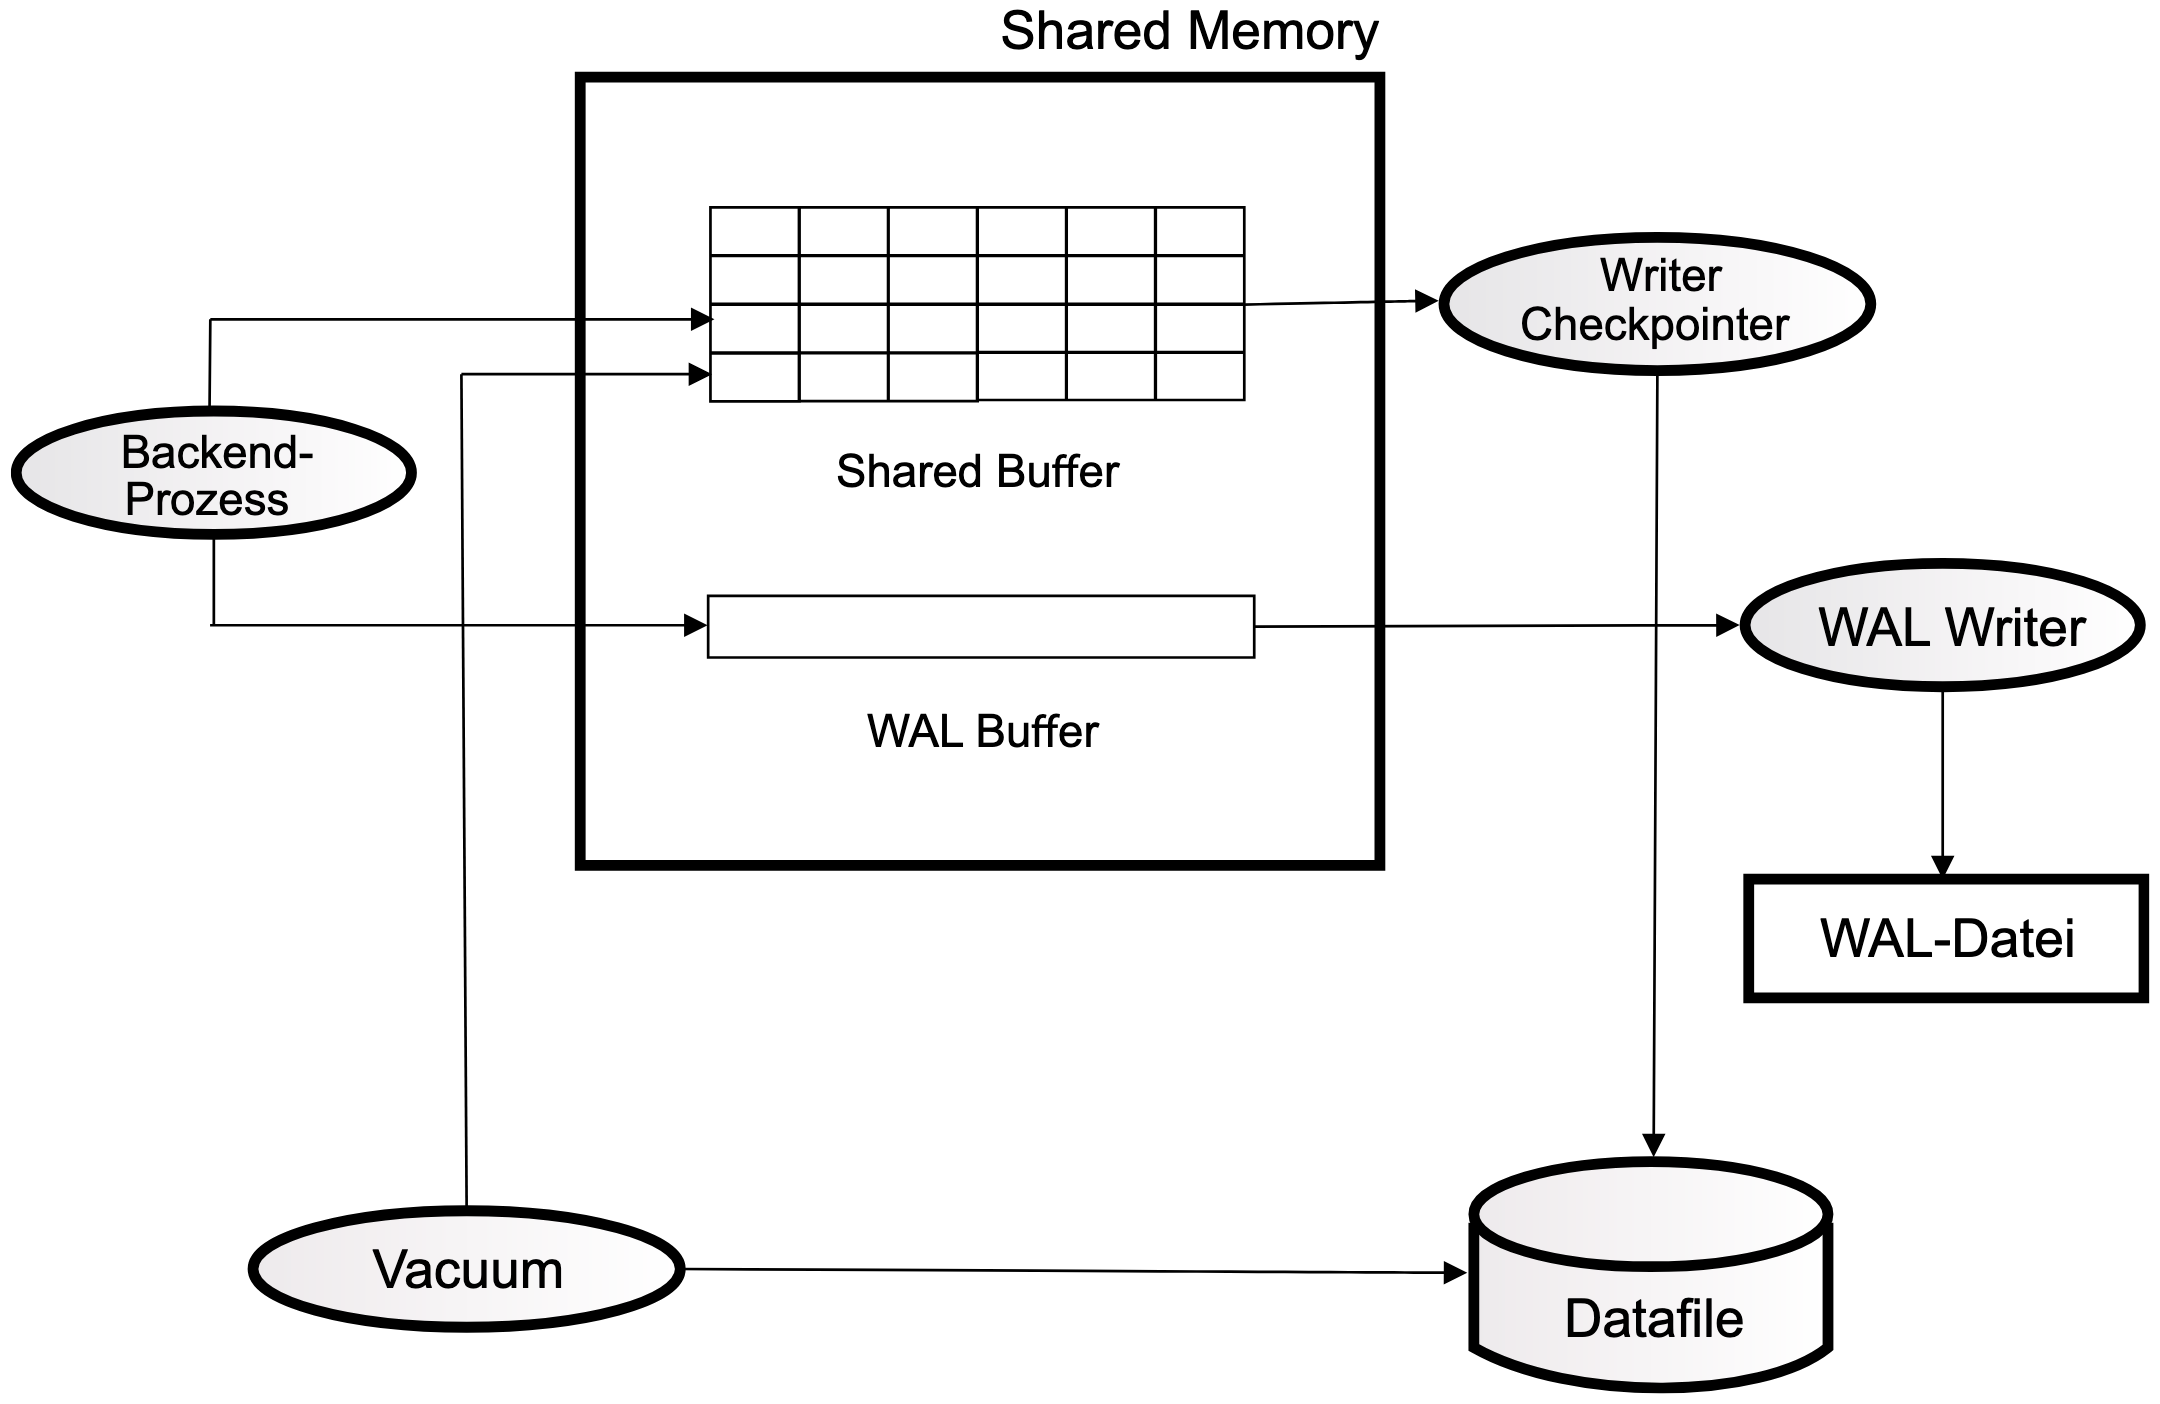
\includegraphics[width=\textwidth]{img/PostgreSQL Aufbau.png}
\caption{PostgreSQL Architektur. Quelle: \cite{Froehlich2022} S. 33 Bild 4.1}
\label{fig:Architektur}
\end{figure}

PostgreSQL besteht aus einer Kombination von Speicher und Prozessen. Bei Unix-Systemen sind diese Prozesse eigenständig, während sie bei Windows als Threads umgesetzt werden. Die wichtigsten Prozesse, die die Funktionalität von PostgreSQL abbilden, sind:
\begin{description}
    \item[Postmaster:] Der Hauptprozess, der die Verwaltung der anderen Prozesse übernimmt.
    \item[Checkpointer:] Dieser Prozess sorgt dafür, dass alle Änderungen in der Datenbank regelmäßig auf die Festplatte geschrieben werden.
    \item[Writer:] Verantwortlich für das Schreiben von geänderten Datenblöcken auf die Festplatte.
    \item[WAL Writer:] Handhabt das Schreiben von Transaktionsdaten in die Write-Ahead Log (WAL).
    \item[Autovacuum Launcher:] Dieser Prozess führt automatische Bereinigungen der Datenbank durch.
    \item[Archiver:] Archiviert die WAL-Dateien für eine verbesserte Rückverfolgbarkeit und Monitoring, besonders wichtig in produktiven Systemen.
    \item[Stats Collector:] Sammelt statistische Daten über die Nutzung von Sessions und Tabellen.
    \item[BGWorker:] Übernimmt verschiedene Hintergrundaufgaben.
\end{description}

\begin{figure}[h]
\centering
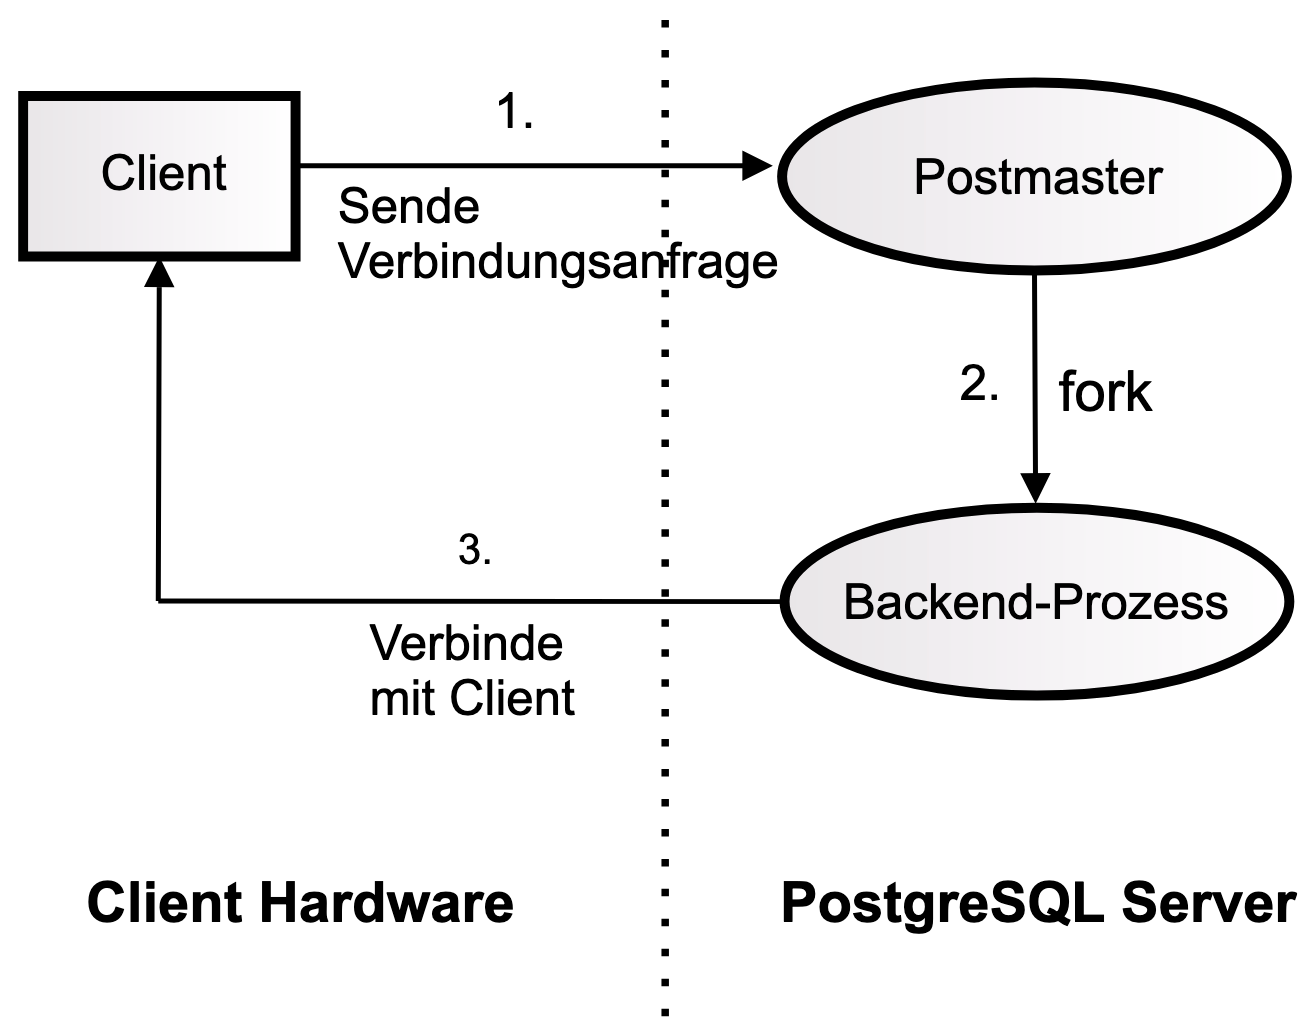
\includegraphics[width=\textwidth]{img/PostgreSQL Verbindungsaufbau.png}
\caption{Verbindungsaufbau von Client zum Server. Quelle: \cite{Froehlich2022} S. 35 Bild 4.3}
\label{fig:Verbindungsaufbau}
\end{figure}

Beim Aufbau einer Verbindung durch einen Client erstellt der Postmaster-Prozess nach erfolgreicher Authentifizierung und Autorisierung einen eigenen Backend-Thread. Die maximale Anzahl gleichzeitig aktiver Backend-Threads ist limitiert (Standard 100), was bedeutet, dass nach Erreichen dieser Grenze weitere Verbindungen abgelehnt werden.

\subsubsection{Speicherverwaltung und Performanceoptimierung}
Die Verwaltung von Speicher und die Optimierung der Zugriffszeiten auf Daten sind entscheidend für die Leistung von PostgreSQL. Da das Lesen von Daten von einer Festplatte vergleichsweise zeitaufwendig ist, setzt PostgreSQL auf verschiedene Mechanismen zur Verbesserung der Performance.

\begin{figure}[h]
\centering
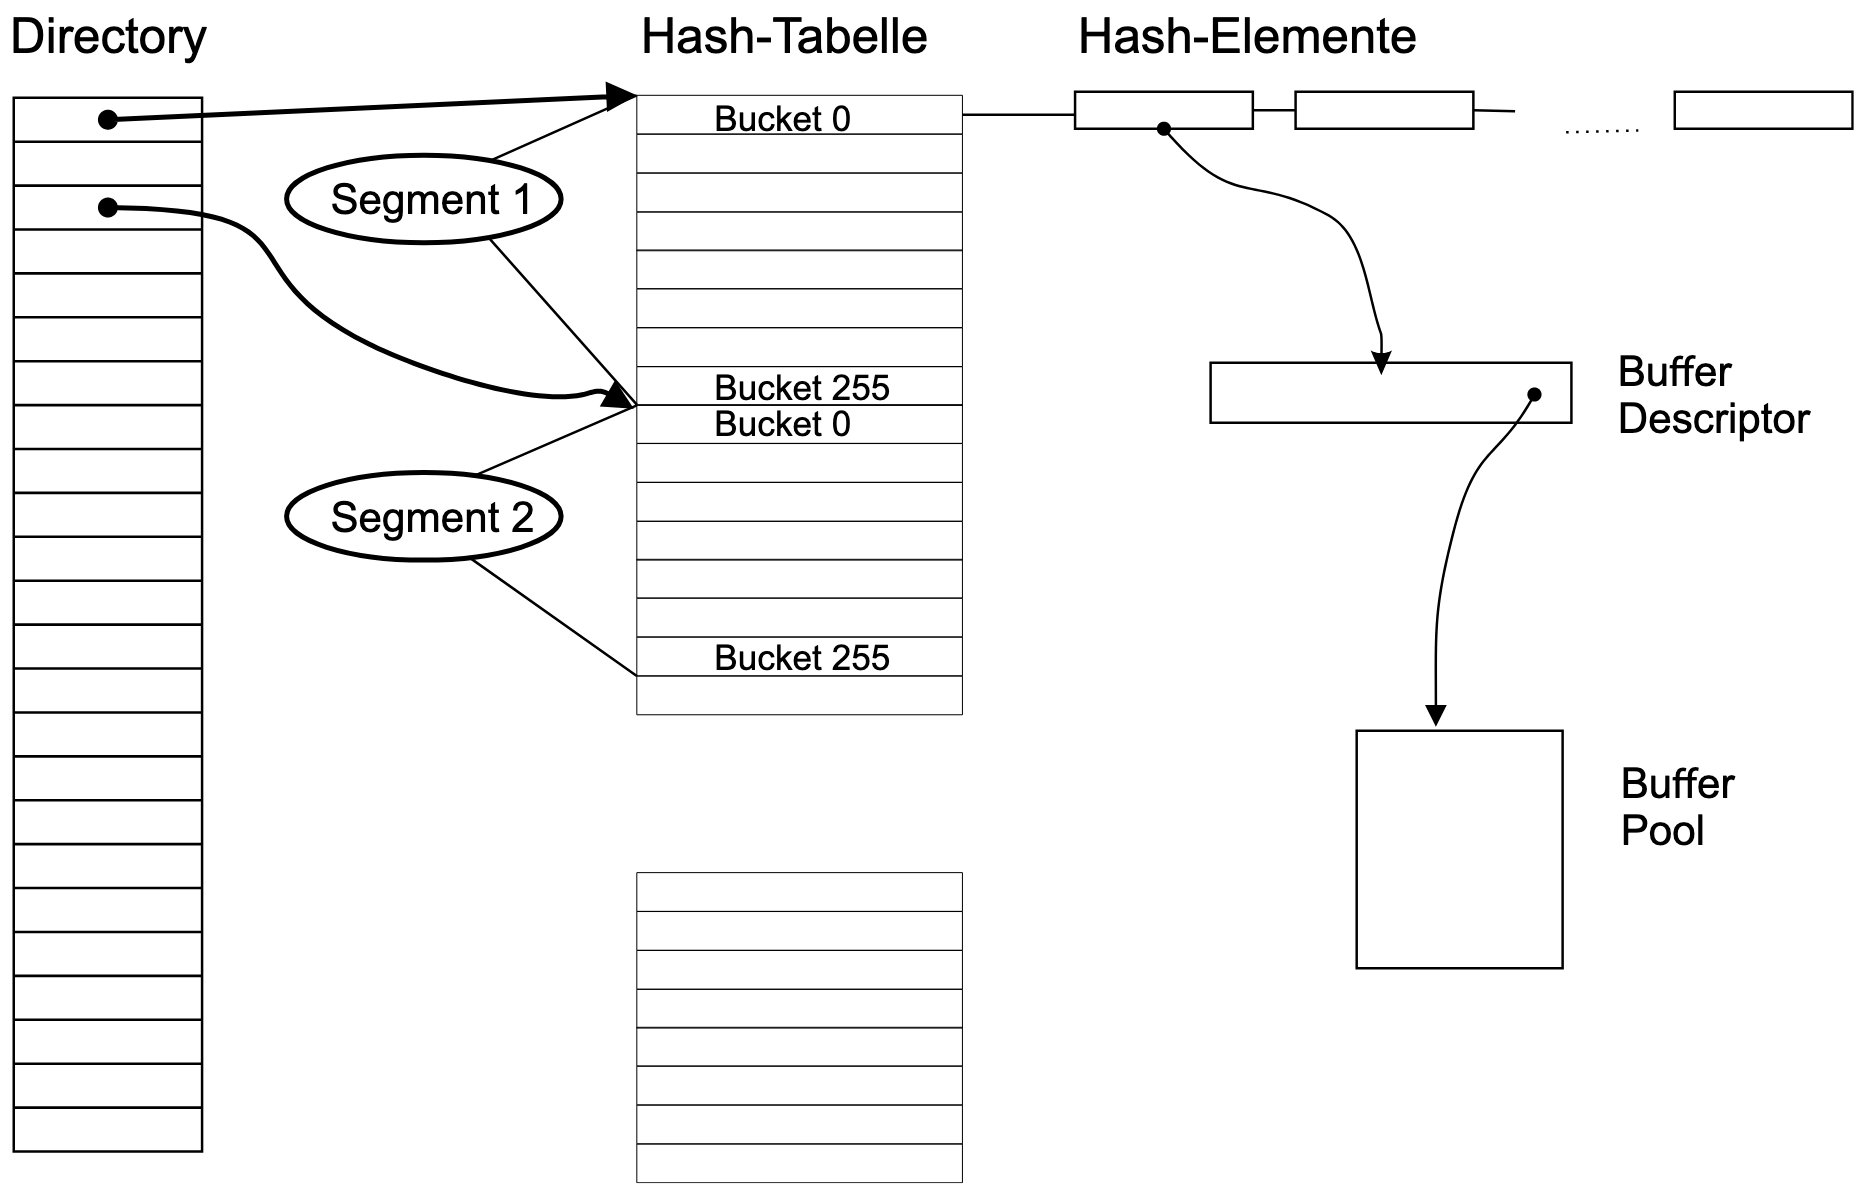
\includegraphics[width=\textwidth]{img/PostgreSQL Speciheraufbau.png}
\caption{PostgreSQL Speicherarchitektur. Quelle:  \cite{Froehlich2022} S. 37 Bild 4.4}
\label{fig:Speicheraufbau}
\end{figure}

\paragraph{Geteilter Speicher (Shared Buffer)}
Der Shared Buffer in PostgreSQL dient dazu, die Anzahl der Operationen auf der Festplatte zu reduzieren, indem er schnellen Speicher im RAM bereitstellt. Er besteht aus einer Hash-Tabelle, Hash-Elementen, einer Bufferbeschreibung und einer Buffersammlung. Die Hash-Tabelle ermöglicht ein schnelles Auffinden von Datensätzen, indem Hashwerte in Segmenten sortiert werden. Diese Segmente können sehr schnell durchsucht werden, da ihre Länge fest ist, was effiziente Speicherzugriffe ermöglicht.

Die Bufferbeschreibung enthält wichtige Steuerungsvariablen, wie z.B. den \code{\url{usage count}}, der die Relevanz eines Datensatzes im Speicher angibt. Der Speicherbereinigungsprozess (Eviction Process) durchsucht regelmäßig den Buffer nach irrelevanten Blöcken. Blöcke, die als irrelevant eingestuft werden, können überschrieben werden, sobald neuer Speicherplatz benötigt wird.

\paragraph{WAL Buffer und Checkpoints}
Der \ac{wal} Buffer ist darauf ausgelegt, Daten effizient auf die Festplatte zu schreiben. Dadurch müssen schreibende Prozesse nicht auf die tatsächliche Schreiboperation warten, sondern können die zu schreibenden Daten in den Buffer verlagern. Der \ac{wal} Buffer wird in regelmäßigen Intervallen (Standard 200 Millisekunden) überprüft und die Daten werden im Permanentspeicher gesichert, um die Ausfallsicherheit zu gewährleisten.

\code{Insert}-, \code{Update}- und \code{Delete}-Anweisungen werden über den \ac{wal}-Buffer verarbeitet. Diese Anweisungen werden in sogenannten \ac{wal}-Records gespeichert und sichern den Zustand der Daten auch bei einem Systemausfall. Ein Checkpoint, der den Speicherinhalt endgültig auf die Festplatte schreibt, wird unter bestimmten Bedingungen ausgeführt, wie etwa nach Ablauf eines festgelegten Intervalls, Erreichen einer bestimmten Buffergröße oder dem manuellen Auslösen eines Checkpoints.

\paragraph{Mehrere Datenblockversionen und Defragmentierung}

PostgreSQL unterstützt die gleichzeitige Bearbeitung von Datensätzen durch mehrere Sessions. Um sicherzustellen, dass sich die Sessions nicht gegenseitig beeinträchtigen, erhalten Datensätze eine Versionsnummer. Diese ermöglicht es, bei gleichzeitigen Abfragen und Bearbeitungen konsistente Daten bereitzustellen. Wenn eine Abfrage gestartet wird, kann anhand der Versionsnummer bestimmt werden, welcher Datensatz zum Zeitpunkt des Abfragestarts aktuell war.

Alte Datensätze, die nicht mehr benötigt werden, werden gelöscht, wodurch Lücken in der Tabelle entstehen. Diese Lücken werden durch den Autovacuum-Prozess freigegeben, sodass der Speicher für neue Datenblöcke verwendet werden kann. Bei Bedarf führt PostgreSQL ein \code{fullvacuum} durch, der die Tabelle vollständig defragmentiert, um Speicherplatz zurückzugewinnen und die Integrität der Versionsnummern zu gewährleisten.

\subsubsection{Permanentspeicherverwaltung}

Die Datenbanken von PostgreSQL werden im Verzeichnis \code{base} gespeichert, während der Tablespace in einem separaten Verzeichnis liegt. Tabellen und Indizes werden in Dateien von maximal einem Gigabyte Größe gespeichert; bei Überschreiten dieser Größe wird eine weitere Datei angelegt. Zusätzlich werden Dateien mit den Endungen \code{\_fsm} (Free Space Map) zur Adressierung des freien Speicherplatzes und \code{\_vm} (Visibility Map) zur Markierung von veralteten Datensätzen gepflegt.

Die Datenblocksammlung (Page) enthält Pointers auf die tatsächlichen Datenblöcke (Tuples). Jeder Datenblock wird durch eine Kombination aus der Datenblocksammlungsnummer und dem Offset des Pointers identifiziert. \cite{Froehlich2022}

\subsection{Exkurs: MongoDB}
MongoDB ist eine führende dokumentenorientierte NoSQL-Datenbank, die sich durch ihre Flexibilität und Skalierbarkeit auszeichnet. Sie wurde entwickelt, um einige der Einschränkungen traditioneller relationaler Datenbanken zu überwinden und bietet eine leistungsfähige Lösung für Anwendungen, die große Mengen an unstrukturierten oder semi-strukturierten Daten verarbeiten müssen. Im Gegensatz zu relationalen Datenbanken, die auf einem festen Schema basieren, erlaubt MongoDB ein dynamisches, schemaloses Datenmodell, das sich ideal für moderne, agile Entwicklungsprozesse eignet. In diesem Exkurs werden die Architektur und die technischen Merkmale von MongoDB detailliert beleuchtet, um deren Eignung für das \ac{nomtis}-Projekt zu bewerten.

\subsubsection{Speicherstruktur und Organisation}
MongoDB speichert Daten im \ac{bson}-Format, einem binären Format, das speziell für die Speicherung von Dokumenten mit \ac{json}-Syntax entwickelt wurde. \ac{bson} bietet eine effiziente Speicherung und Verarbeitung von Dokumenten, da es im Vergleich zu herkömmlichem \ac{json} kompakter und schneller zu verarbeiten ist. \ac{bson}-Dokumente können direkt in \ac{json} konvertiert werden, was die Integration mit Anwendungen erleichtert, die \ac{json} verwenden.

Die Speicherorganisation in MongoDB ist hierarchisch aufgebaut:
\begin{description}
    \item[Datenbank:] An der Spitze steht eine Datenbank, die mehrere Sammlungen (engl. Collections) enthalten kann.
    \item [Katalog:] Darunter befindet sich der Katalog, der Informationen über die Sammlungen und Indizes speichert.
    \item [Sammlung (engl. Collection)]: Eine Sammlung ist eine Gruppe von Dokumenten, die thematisch zusammengehören und ähnliche Strukturmerkmale aufweisen.
    \item [Dokument:] Auf der untersten Ebene steht das Dokument, das die eigentlichen Daten enthält.
\end{description}

\subsubsection{Katalog und Speicherverwaltung}

Der Katalog von MongoDB ist für die Verwaltung der Metadaten von Sammlungen und Indizes verantwortlich. Es gibt zwei Arten von Katalogen:
\begin{description}
    \item[Persistenter Katalog:] Dieser speichert Informationen dauerhaft auf der Festplatte und stellt sicher, dass Metadaten auch nach einem Neustart des Systems verfügbar bleiben. Der persistente Katalog wird in BSON-Dateien mit der Endung \code{\_mdb\_catalog} gespeichert und enthält Details über die Eigenschaften und Indizes der Sammlungen.
    \item [Memory-Katalog:] Der Memory-Katalog hält die Metadaten im RAM vor, um schnellen Zugriff zu gewährleisten und Ladezeiten zu minimieren. Operationen wie das Erstellen, Suchen, Iterieren und Schließen von Sammlungen werden im Memory-Katalog durchgeführt.
\end{description}

Um Dateninkonsistenzen zu vermeiden, wird der Memory-Katalog regelmäßig mit dem persistenten Katalog synchronisiert. Eine Versionsverwaltung stellt sicher, dass Änderungen korrekt nachvollzogen werden können, ohne dass es zu Lese-Schreib-Kollisionen kommt. MongoDB verwendet dabei das Copy-on-Write-Prinzip, bei dem nur dann eine Kopie des Datensatzes erstellt wird, wenn tatsächlich Änderungen vorgenommen werden. Dies minimiert den Speicherbedarf und erhöht die Effizienz.

\subsubsection{Speicherverwaltung und Defragmentierung}
Beim Löschen eines Eintrags in MongoDB erfolgt dieser Prozess in zwei Schritten:
\begin{enumerate}
    \item Löschen des Katalogeintrags: Zunächst wird der Eintrag sowohl im Memory-Katalog als auch im persistenten Katalog entfernt. Ein Verweis auf die Sammlung wird an den sogenannten \glqq Reaper\grqq{} übergeben, um sicherzustellen, dass keine neuen Zugriffe auf die Sammlung erfolgen, während aktive Lesezugriffe abgeschlossen werden.
    \item Endgültiges Löschen: Nachdem sichergestellt wurde, dass kein Rollback erfolgen kann, der die Daten der Sammlung wiederherstellen könnte, werden die Daten endgültig gelöscht.
\end{enumerate}

Freier Speicher, der durch das Löschen von Daten entsteht, wird in regelmäßigen Abständen für neue Datensätze freigegeben. Wenn der Speicher fragmentiert wird und viele kleine Lücken entstehen, führt MongoDB eine Defragmentierung durch. Dieser Prozess ordnet den Speicher neu an, kann jedoch Lese- und Schreiboperationen blockieren, was die Performance beeinträchtigen könnte. Daher sollte die Defragmentierung möglichst selten durchgeführt werden.

\subsubsection{Indizes und Abfragen}
Indizes in MongoDB werden hauptsächlich als B-Baum-Strukturen gespeichert, die eine effiziente Suche und Sortierung von Daten ermöglichen. Ein B-Baum-Index speichert die Daten strukturiert, ähnlich wie ein Dokument, und ermöglicht schnelle Zugriffe auf häufig abgefragte Felder. MongoDB erlaubt es auch, benutzerdefinierte Speicherstrukturen für Indizes zu erstellen, um spezifische Anwendungsanforderungen zu erfüllen. \cite{IamXander2024} \cite{themattman2024}

\subsubsection{BSON - Binary JSON}

\ac{bson} ist das zugrunde liegende Format für die Speicherung von Dokumenten in MongoDB. Es handelt sich dabei um ein binäres Format, das sogenannte Key-Value-Paare speichert und direkt in \ac{json} konvertiert werden kann. \ac{bson} ist jedoch deterministischer als \ac{json}, da es keine Flexibilität in der Darstellungsform bietet. Dies bedeutet, dass ein Datensatz in \ac{bson} immer in einer einzigen, festen Form dargestellt wird.

Ein \ac{bson}-Dokument beginnt immer mit einem 32-Bit-Ganzzahlwert, der die Länge des Dokuments angibt, und endet mit einem Null-Byte. Aufgrund dieser Struktur kann ein \ac{bson}-Dokument maximal ca. 2,147 Gigabyte an Daten umfassen. Die verschiedenen Datentypen, die \ac{bson} unterstützt, umfassen unter anderem:
\begin{description}
    \item[Int32 und Int64:] 4- bzw. 8-Byte lange Ganzzahlen.
    \item[Double:] 8-Byte lange Gleitkommazahlen nach dem IEEE 754-Standard.
    \item[Decimal128:] 16-Byte lange Gleitkommazahlen für hohe Präzision.
    \item[Array:] Ein Feld, das eine Liste von Werten speichert, wobei die Elemente wie Dokumente behandelt werden.
    \item[Null-Wert:] Ein spezieller Marker, der das Fehlen eines Wertes kennzeichnet.
    \item[Min- und Max-Schlüssel:] Marker, die den minimalen bzw. maximalen Wert eines Feldes darstellen.
\end{description}

Die strikte Struktur von \ac{bson} sorgt für eine konsistente und effiziente Speicherung und Verarbeitung von Dokumenten, was MongoDB zu einer leistungsfähigen Lösung für Anwendungen macht, die flexible und skalierbare Datenbanken benötigen. \cite{Velikhov}

\subsection{Diskurs: Vergleich von PostgreSQL und MongoDB für NOMTIS}
Die Auswahl der geeigneten Datenbanklösung ist ein zentraler Aspekt bei der Entwicklung von \ac{nomtis}. Da die internen Richtlinien PostgreSQL und MongoDB als verfügbare Optionen vorsehen, ist es entscheidend, die spezifischen Anforderungen von \ac{nomtis} zu analysieren und zu bestimmen, welche der beiden Datenbanken diese am besten erfüllt.

\subsubsection{Technische Anforderungen an NOMTIS}
\ac{nomtis} muss Benachrichtigungen effizient speichern, verwalten und flexibel verarbeiten können. Ein Hauptmerkmal von \ac{nomtis} ist die Fähigkeit, Benachrichtigungen mit potenziell komplexen und verschachtelten Datenstrukturen zu verwalten. Diese Datenstrukturen können variieren und sind oft nicht im Voraus vollständig definiert. Zudem sind eine hohe Zuverlässigkeit, Konsistenz und Skalierbarkeit erforderlich, um den Anforderungen eines modernen Benachrichtigungssystems gerecht zu werden.

\subsubsection{PostgreSQL: Technische Stärken und Grenzen}
PostgreSQL ist eine relationale Datenbank, die für ihre starke Unterstützung von \ac{acid}-Transaktionen, Datenintegrität und komplexen relationalen Abfragen bekannt ist. Diese Eigenschaften machen PostgreSQL ideal für Anwendungen, bei denen strenge Konsistenzanforderungen und komplexe Datenbeziehungen im Vordergrund stehen.

Die feste Struktur von PostgreSQL kann jedoch zu Einschränkungen führen, wenn es darum geht, dynamische und verschachtelte Datenstrukturen zu verwalten. Änderungen am Datenmodell erfordern eine Anpassung des Schemas, was in einem dynamischen Umfeld, wie es \ac{nomtis} erfordert, potenziell problematisch sein kann. Zudem ist PostgreSQL weniger effizient im Umgang mit tief verschachtelten oder unvorhersehbaren Datenstrukturen, was die Flexibilität des Systems einschränken könnte.

\subsubsection{MongoDB: Flexibilität und Skalierbarkeit}
MongoDB hingegen ist eine dokumentenorientierte NoSQL-Datenbank, die sich durch ihre schemalose Architektur und hohe Flexibilität auszeichnet. Die Speicherung erfolgt im BSON-Format, das eine effiziente Handhabung von \ac{json}-ähnlichen Dokumenten ermöglicht. Diese Struktur erlaubt es, Daten ohne festes Schema zu speichern, was für \ac{nomtis} von Vorteil ist, da die Benachrichtigungen beliebig komplexe und verschachtelte Daten enthalten können.

Ein weiterer zentraler Vorteil von MongoDB ist seine horizontale Skalierbarkeit. MongoDB unterstützt das sogenannte \glqq Sharding \grqq, bei dem Daten über mehrere Server verteilt werden, um eine hohe Verfügbarkeit und Performance sicherzustellen. Diese Fähigkeit zur horizontalen Skalierung ist besonders in einer Umgebung wie der \ac{sit} von Bedeutung, wo das Datenvolumen und die Anzahl der Nutzer kontinuierlich wachsen können.

Laut einer Untersuchung der MongoDB-Datenbank von Anjali Chauhan bietet MongoDB darüber hinaus eine hohe Leistung durch die Verwendung eingebetteter Datenmodelle, die E/A-Aktivitäten reduzieren, sowie durch Indizes, die schnellere Abfragen ermöglichen. \cite{Chauhan2019}
Diese Leistungsmerkmale machen MongoDB besonders geeignet für Anwendungen, die auf hohe Geschwindigkeit und effizienten Datenzugriff angewiesen sind.

\subsubsection{Schlussfolgerung: PostgreSQL als geeignete Wahl für Sensora}
Im Projekt Sensora ergibt sich aus den strukturellen Anforderungen und den funktionalen Zugriffsmustern ein klarer Bedarf an einem relationalen, transaktional konsistenten Datenbanksystem. Die Datenstruktur ist vordefiniert und weitgehend stabil. Pflanzen, Sensoren, Aktoren, Gruppen und Räume bilden klar abgegrenzte Entitäten mit definierten Beziehungen zueinander. Diese Relationen sind nicht nur logisch konzipiert, sondern stellen funktionale Notwendigkeiten dar – etwa wenn Sensoren bestimmten Pflanzen zugeordnet sind oder Aktionen nur innerhalb definierter Gruppenzugehörigkeiten zulässig sind.

Die Abfrageanforderungen im operativen Betrieb bestehen aus einer Mischung aus punktuellen Zugriffen (etwa auf aktuelle Sensorwerte oder Soll-Ist-Vergleiche) und zeitbasierten Auswertungen über große Datenmengen – insbesondere für die letzten 24 Stunden. Diese Anforderungen sind auf ein konsistentes, indexoptimiertes Schema angewiesen, das Joins effizient unterstützt und sich nicht durch Schema-Flexibilität, sondern durch strukturelle Integrität auszeichnet. Gleichzeitig ist paralleler Zugriff durch mehrere Microservices erforderlich, sodass Transaktionssicherheit und Isolation nicht nur erwünscht, sondern notwendig sind, um Inkonsistenzen bei konkurrierenden Schreiboperationen zu vermeiden.

PostgreSQL bietet genau für diese Art von Workload die passende Grundlage. Die stark normierten Strukturen des Sensora-Datenmodells profitieren von PostgreSQLs ausgefeilter Optimierung relationaler Abfragen, der zuverlässigen Durchsetzung referenzieller Integrität sowie der Möglichkeit, durch gezieltes Indexing auf Zeitstempel-Feldern hochfrequente historische Abfragen performant abzubilden. Selbst bei wachsendem Datenvolumen lassen sich durch Partitionierung oder die spätere Ergänzung durch TimescaleDB – ohne Verlassen der PostgreSQL-Basis – die Performanceanforderungen langfristig erfüllen, ohne strukturelle Kompromisse einzugehen.

Die fehlende Notwendigkeit für dynamische Schemas, polymorphe Dokumente oder eingebettete Strukturen eliminiert die Hauptargumente für ein dokumentenbasiertes System wie MongoDB. Vielmehr würde dessen Flexibilität in diesem Kontext eher potenzielle Inkonsistenzen begünstigen und zusätzliche Validierungslogik auf Anwendungsebene erforderlich machen – ein Mehraufwand, der durch das klar strukturierte Datenmodell nicht gerechtfertigt ist.

In Summe ist PostgreSQL damit nicht nur die technisch bessere Wahl, sondern die natürlichere Fortsetzung der bereits im Projektdesign angelegten Prinzipien: strukturierte, konsistente und integrierte Datenhaltung, auf die performant und sicher gleichzeitig von vielen Systemkomponenten zugegriffen werden kann.

	%%Auswahl der Technologien für eine Kompüonente des Projektes, basierend auf den Anforderungen, die in der vorherigen Sektion definiert wurden (Zentral für die Arbeit)
\section{IoT Device}
Das IoT Device ist ein zentraler Bestandteil des Projektes. Es ist dafür verantwortlich, die Daten von den Sensoren zu sammeln und an die Cloud zu übertragen. In diesem Abschnitt werden die Technologien ausgewählt, die für das IoT Device verwendet werden sollen. Die Auswahl erfolgt auf Basis der Anforderungen, die in der vorherigen Sektion definiert wurden.
\subsection{Verfügbare Technologien}
Die folgenden Technologien sind verfügbar.
\subsection{State of the Art Technologie}
Die Technologie 1 ist State of the Art und wird oft für IoT Devices verwendet.
\subsection{Vergleich von Technologien}
Die Technologien erfüllen die Anforderungen wie folgt:
\begin{itemize}
    \item Technologie 1: erfüllt die Anforderungen A, B und C.
    \item Technologie 2: erfüllt die Anforderungen A, B und D.
    \item Technologie 3: erfüllt die Anforderungen A, C und D.
\end{itemize}
\subsection{Auswahl der Technologie}
Die Technologie 1 wird ausgewählt, da sie die Anforderungen A, B und C erfüllt. Die Technologie 2 wird nicht ausgewählt, da sie die Anforderungen A, B und D erfüllt, aber nicht so gut wie Technologie 1. Die Technologie 3 wird ebenfalls nicht ausgewählt, da sie die Anforderungen A, C und D erfüllt, aber nicht so gut wie Technologie 1.
%Alternativ: Die technologie wird trotz ihre Status als State of the Art nicht ausgewählt, da sie die Anforderungen nicht ausreichend erfüllt.
	
	\newpage
	
	\chapter{Umsetzung}
	\section{Beschreibung des Datenbankaufbaus}
Die Datenbank des Systems Sensora ist im Schema sensora organisiert und verfolgt eine klar strukturierte, relationale Modellierung mit durchdachter Referentialität und Typisierung. Sie unterstützt die zentralen Funktionen des Systems wie Benutzerverwaltung, Gruppenzugehörigkeit, Raum- und Pflanzenzuordnung sowie Sensor- und Steuerdaten.
\newpage
\begin{figure}[H]
\centering
%  \includesvg[width=\linewidth, height=0.9\textheight, keepaspectratio,inkscapelatex=false]{img/Datenbank Diagramm.svg}
  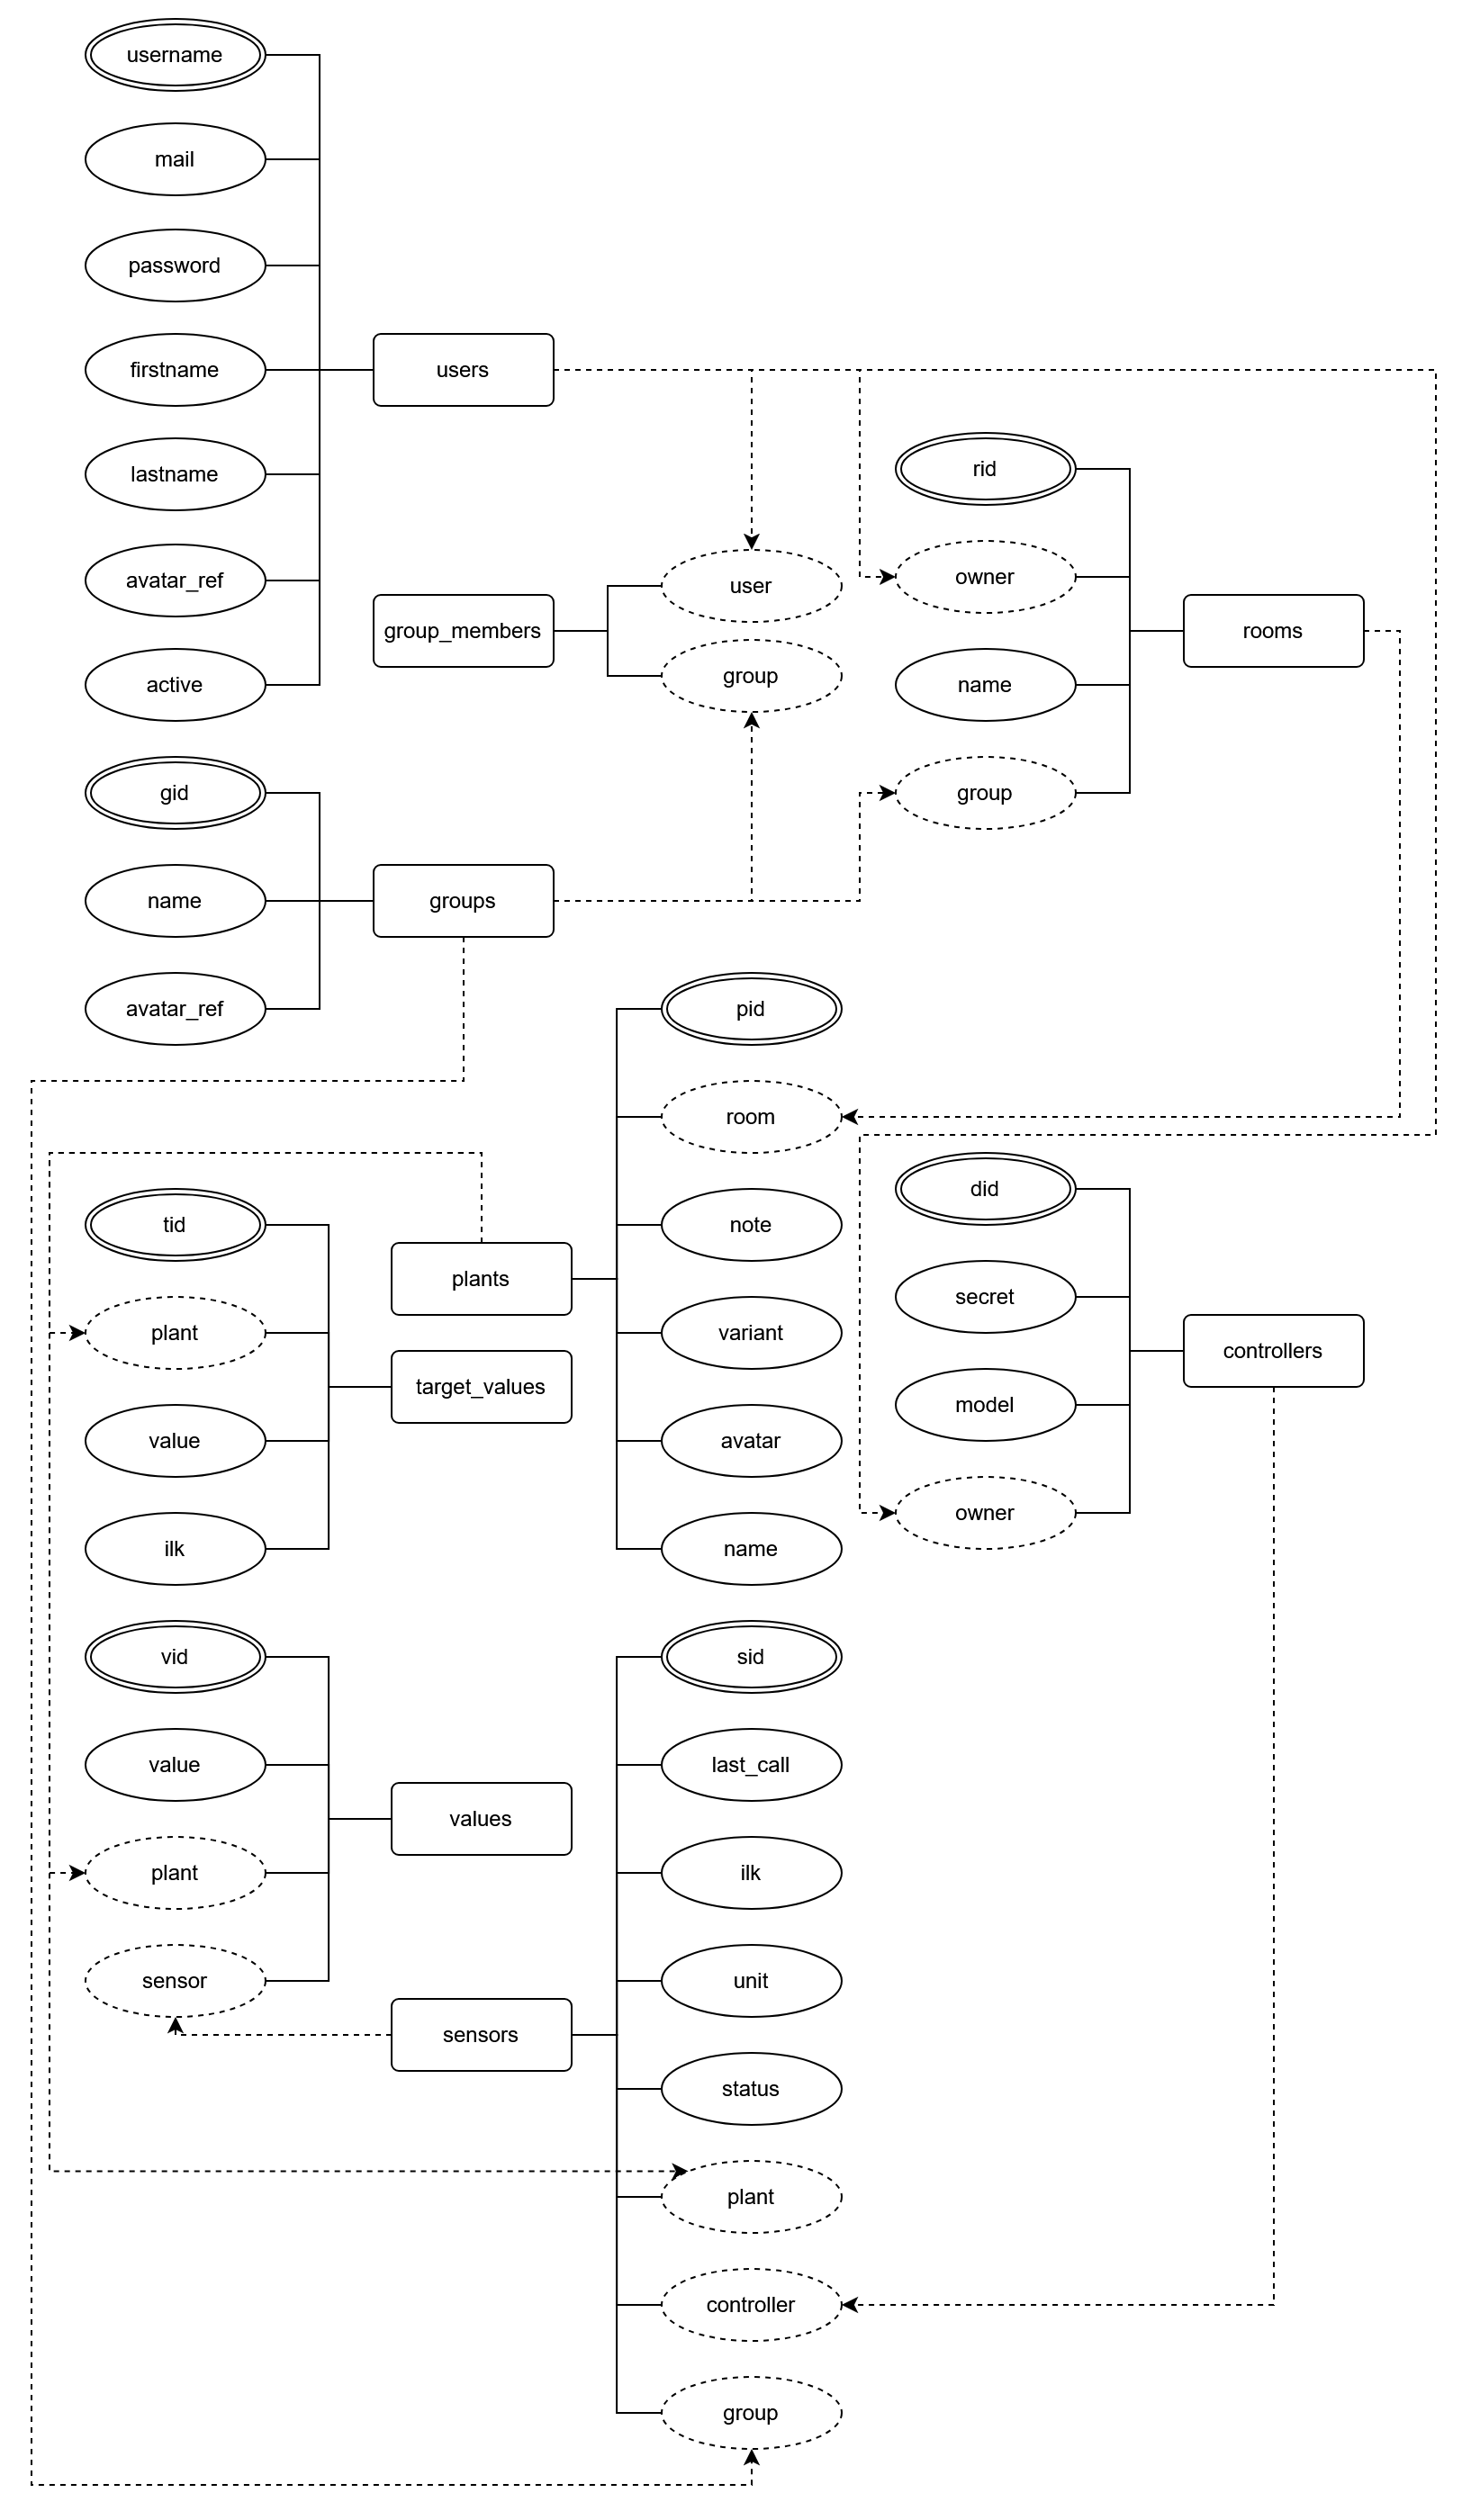
\includegraphics[width=\linewidth, height=0.9\textheight]{img/Datenbank Diagramm.png}
\caption{Sensora Datenbank Struktur}
\label{fig:sensora_datenbank}
\end{figure}
\newpage

\subsection{Struktur und Besonderheiten}
\begin{description}
    \item[Benutzerverwaltung:]
    Die Tabelle users bildet die zentrale Entität für Benutzer ab. Jeder Benutzer besitzt Pflichtangaben sowie einen referenzierten Avatar aus dem dedizierten ENUM-Typ sensora.avatar. Die E-Mail-Adresse ist eindeutig.
    \item[Gruppen \& Mitgliedschaften:]
    Gruppen (groups) können mehrere Mitglieder haben, realisiert durch die Join-Tabelle group\_members. Diese bildet eine klassische Many-to-Many-Beziehung zwischen Nutzern und Gruppen ab.
    \item[Räume \& Pflanzen:]
    Räume (rooms) können Gruppen zugeordnet sein und besitzen jeweils einen Eigentümer. Pflanzen (plants) sind immer einem Raum zugeordnet und dienen als Ankerpunkt für Messwerte.
    \item [Sensorik \& Steuerung:]
    Sensoren (sensors) sind mit Controllern (controllers) verknüpft und optional direkt mit einer Pflanze oder Gruppe verbunden. Jeder Sensor verwendet den ENUM-Typ sensora.status, um seinen Zustand zu klassifizieren.
    \item [Zielwerte \& Messdaten:]
    Pflanzen können über target\_values Zielgrößen definieren. Tatsächliche Messwerte werden in der Tabelle values gespeichert und jeweils einem Sensor sowie einer Pflanze zugeordnet.
\end{description}

\subsection{Technische Merkmale}
\begin{itemize}
    \item Es kommen ENUM-Typen zum Einsatz, um Felder wie Avatar und Status typensicher und standardisiert zu definieren.
    \item Sämtliche Fremdschlüsselbeziehungen nutzen CASCADE-Strategien zur Pflege von Konsistenz (z.B. beim Löschen von Benutzern oder Pflanzen).
    \item Indizes auf eindeutige Felder (z.B. mail, secret) erhöhen die Performanz gezielter Abfragen.
    \item Die Nutzung von Timestamps mit Standardwerten erlaubt eine automatische Protokollierung von Ereignissen wie Sensoraktivität.
\end{itemize}

Diese Datenbankstruktur ermöglicht eine flexible, erweiterbare und gleichzeitig robuste Grundlage für die Backend-Logik und garantiert eine nachvollziehbare Abbildung der fachlichen Entitäten.
	%%Hier wird alles beschrieben und erklärt, was während in der Praxis passiert ist und gemacht wurde.
\section{Umsetzung des IoT Devices}
Das IoT Device wurde von einer Person als Hauptentwickler und mehreren Unterstützenden Entwicklern erstellt.
    \subsection{Hardware}:
    Für die Hardware wurde ein fertiger Bausatz von Alibaba gekauft, der alle benötigten Komponenten enthielt.
    Darunter ein ESP32, sensoren und eine Pumpe.
    Die Hardware wurde zusammengebaut und testweise in Betrieb genommen, yada yada yada.
    \subsection{Software}:
    Die SOftware wurde in C Entwickelt.
    Es wurden die Komponenten x, y und z implementiert.
    Dabei lief dies gut und das nicht so gut.
   
	\section{Frontendarchitektur und Datenflüsse im System}
Die Frontendarchitektur des smarten Bewässerungssystems wurde nach dem Paradigma komponentenbasierter Webentwicklung realisiert. Ziel war es, eine modular aufgebaute, wartbare und reaktive Benutzeroberfläche zu schaffen, die flexibel auf unterschiedliche Endgeräte und Benutzeranforderungen reagiert. Im Zentrum steht dabei das Framework Vue.js in Verbindung mit dem State-Management-Tool Pinia. Im Folgenden werden die Strukturierung der Views, das Datenflussmodell sowie die Rolle zentraler Technologien im Detail betrachtet.

\subsection{Komponentenbasierte Struktur und Navigationsmodell}
Die Architektur der vorliegenden Anwendung folgt einem komponentenbasierten Ansatz gemäß der Vue.js-Konventionen. Jede View in der Applikation ist als \ac{SFC} implementiert. Eine \ac{SFC} vereint die drei wesentlichen Bestandteile einer Webkomponente in einer Datei: Template, Script und Styles. Das Template definiert die Benutzeroberfläche in HTML-ähnlicher Syntax, das Script implementiert die zugehörige Logik (meist in TypeScript), und der Style-Block regelt das visuelle Layout mittels CSS bzw. Tailwind CSS. Diese Trennung innerhalb einer Datei fördert sowohl die Lesbarkeit als auch die Wiederverwendbarkeit von Komponenten \cite{VueGuide2024}.

Die Views der Anwendung (z. B.	\texttt{HomeView}, 	\texttt{SinglePlantView}, 	\texttt{GroupView}, 	\texttt{SingleSensorView} sowie 	\texttt{PlantListView}) stellen jeweils eigenständige Seiten dar, die durch den Einsatz des Vue Routers dynamisch geladen werden. Jede dieser Views aggregiert untergeordnete Komponenten wie Karten, Dialoge, Navigationsleisten oder Diagramme und bindet dabei die jeweils relevanten Daten aus dem zentralen Zustand.

Die Navigationsstruktur ist hierarchisch aufgebaut. Eine Hauptansicht (\texttt{HomeView}) dient als Einstiegspunkt und aggregiert Informationen aus den verschiedenen Kontexten: Räume, Pflanzen und deren Sensordaten. Ausgehend davon ermöglicht das Routing eine Tiefennavigation bis auf Objektebene, z.\,B. zum Bearbeiten einer bestimmten Pflanze. Dies fördert die kognitive Abbildung realweltlicher Strukturen (Wohnung $\rightarrow$ Raum $\rightarrow$ Pflanze) im digitalen Raum.
 
 \subsection{Pinia als Vermittlungsinstanz zwischen API und Frontend}
 Zur zentralen Zustandsverwaltung kommt Pinia zum Einsatz, welches das offizielle State-Management-System für Vue 3 darstellt \cite{Vuex, Allotey2023}. Anders als bei Vuex erfolgt die Definition eines Stores in Pinia mittels der Funktion \texttt{defineStore}, wobei sowohl State als auch Actions und Getters kapsuliert definiert werden. Diese Struktur unterstützt sowohl die Modularität als auch die Wiederverwendbarkeit der Zustandslogik.
 
 Pinia fungiert im Anwendungskontext als Puffer und vermittelnde Instanz zwischen dem Frontend und der REST-API. Die Stores agieren als Cache: sie speichern persistente Daten über Komponentenlebenszyklen hinweg und reduzieren dadurch die Anzahl notwendiger API-Anfragen. Dies verbessert sowohl die Performance als auch die Benutzererfahrung, da viele Interaktionen lokal bedient werden können. Persistiert wird der Zustand mittels \texttt{pinia-plugin-persistedstate} im \texttt{localStorage}, wodurch Informationen wie eingeloggte Nutzer oder selektierte Objekte auch bei einem Seitenreload erhalten bleiben.
 
 In der Applikation existieren getrennte Stores für Benutzerinformationen (\texttt{user.ts}), Authentifizierung (\texttt{auth.ts}), Pflanzen (\texttt{plant.ts}), Geräte (\texttt{device.ts}) und Räume (\texttt{room.ts}). Jeder Store definiert spezifische Actions, typischerweise asynchrone Methoden, alle die API-Schnittstellen repräsentieren und einige Weitere. Wenn Änderungen stattfinden, werden diese immer direkt an die API gesendet. Wenn Daten abgefragt werden, wird zuerst geprüft ob sie im Store verfügbar sind, wenn nicht wird erst eine Anfrage ans Backend gestellt. Diese neuen Daten werden dann gespeichert und automatisch in die andern Stores synchronisiert. 
 
 Optional kann eine Aktion auch mit einem \texttt{force}-Flag aufgerufen werden, welches eine explizite Aktualisierung erzwingt. Dies geschieht Beispielsweise bei "Pull-to-Refresh". Diese Strategie erlaubt einen kontrollierten Kompromiss zwischen Reaktivitiät und Ressourceneffizienz.
 
Um die Daten vor missbräuchlichen Zugriff zu schützen, wurde eine explizite Clear-Strategie implementiert. Bei Logout oder Benutzerwechsel werden alle Stores mittels \texttt{clearData()} zurückgesetzt, wodurch Persistenzdaten und Zustand explizit gelöscht werden. Das explizite Löschen ist auch über die Benutzereinstellung möglich.

\subsection{Datenfluss nach dem Flux-Prinzip}

Die Applikation folgt in ihrer Zustandslogik dem Flux-Prinzip, das ursprünglich von Facebook zur Beherrschung komplexer UI-Zustände vorgeschlagen wurde. Charakteristisch für dieses Architekturmodell ist ein strikt unidirektionaler Datenfluss: Interaktionen in der Benutzeroberfläche führen zu sogenannten Actions, die logische Operationen wie API-Aufrufe oder Validierungen auslösen. Die dabei gewonnenen Daten werden im zentralen State-Container gespeichert, welcher wiederum die View reaktiv aktualisiert. Dieser Ablauf lässt sich als Kette beschreiben: \texttt{UI $\rightarrow$ Action $\rightarrow$ Backend $\rightarrow$ Store $\rightarrow$ UI} \cite{Flux, facebook_flux}.

Die Trennung der Zuständigkeiten – insbesondere zwischen Anzeige, Logik und Datenhaltung – begünstigt eine konsistente und vorhersehbare Datenverwaltung. Da alle Zustandsveränderungen über dedizierte Actions verlaufen und sich zentral nachverfolgen lassen, verbessert das Modell sowohl die Testbarkeit als auch die Wartbarkeit der Anwendung \cite{Flux}. In Kombination mit Pinia, das als modernes, modulbasiertes State-Management-Tool agiert, ergibt sich eine Architektur, die eng an Flux angelehnt ist, dabei jedoch die Komplexität traditioneller Implementierungen (z.\,B. Redux) vermeidet.

 \subsection{Fazit}
 Die vorliegende Frontend-Architektur basiert auf einem robusten Zusammenspiel modularer Komponenten, zentralisiertem State-Management mit Pinia und asynchroner Datenkommunikation. Die Trennung von Zustandslogik und Darstellung, kombiniert mit der Persistenz und Synchronisationsstrategie, gewährleistet eine wartbare und benutzerfreundliche Applikation.
 
 
	\section{Benutzerzentriertes Design und UI/UX im Frontend}

Im Bezug auf die theoretische Erläuterung zentraler Konzepte wie \ac{UCD} und den Usability-Heuristiken nach Nielsen sowie dem \ac{UX}-Leitbild des Responsive Designs, wird in diesem Abschnitt die konkrete Umsetzung dieser Prinzipien im Rahmen der Vue.js-basierten Anwendung dargestellt. Ziel ist es, die Überführung theoretischer Vorgaben in praktische Gestaltungslösungen nachvollziehbar zu machen und zu zeigen, wie benutzerzentrierte Entwicklung zur Verbesserung der \ac{UI}-Qualität beiträgt.

\subsection{Anwendung von UCD im smarten Bewässerungssystem}

Die Nutzerforschung erfolgte durch halbstrukturierte Interviews mit VertreterInnen der Zielgruppe (z.\,B. HobbygärtnerInnen, technikaffine Personen). Daraus wurden mehrere Personas abgeleitet, die unterschiedliche Nutzungsmotive wie einfache Bedienung, Transparenz von Sensordaten und Kooperation abbilden. 

Darauf aufbauend wurden Wireframes auf Papier entwickelt, welche die Informationsarchitektur und zentrale Navigationsstrukturen skizzierten. Diese papierbasierten Modelle wurden iterativ angepasst und mit ausgewählten Testpersonen diskutiert. Durch diese formative Evaluation konnte bereits vor der Implementierung auf zentrale Anforderungen reagiert werden.

Auf Basis des Nutzerfeedbacks wurde die Darstellung der Gruppenansicht verbessert. Konkret ergaben sich folgende Anforderungen: Die NutzerInnen wünschten sich eine übersichtliche Darstellung der Gruppen sowie die Möglichkeit, auf einfache Weise die MitgliederInnen einer Gruppe einzusehen, ohne dass zu viele Informationen gleichzeitig auf dem Bildschirm erscheinen. Um diese Bedürfnisse zu erfüllen, wurde die GroupsView als Card-Layout konzipiert.

Diese Card präsentiert auf den ersten Blick nur die wichtigsten Informationen einer Gruppe. Über den Titel oder dem Button können die NutzerInnen die Card bei Bedarf „ausklappen“. Wird der Button gedrückt, erweitert sich die Card dynamisch und zeigt alle zugehörigen MitgliederInnen an. Dies verbessert die Übersichtlichkeit, da nicht alle Details permanent sichtbar sind und die NutzerInnen selbst steuern können, wann sie vertiefte Informationen einsehen.

Besonders benutzerfreundlich ist die neue Lösung auch darin, dass, wenn nur eine einzige Gruppe vorhanden ist, diese Card bereits automatisch ausgeklappt dargestellt wird. Auf diese Weise entfällt ein unnötiger zusätzlicher Klick und der direkte Zugriff auf die Gruppendetails wird erleichtert – ein kleines Detail, das jedoch signifikant zur Verbesserung der User Experience beiträgt.

Eine weitere Optimierung ist auf der SingelPlantView gemacht worden.
Aufgrund Nutzerfeedbacks wurde eine horizontale Linie in das Diagramm integriert, um den Sollwert des Messsatzes optisch darzustellen. Die Linie ermöglicht es den Nutzerinnen und Nutzern sofort zu erkennen, wo sich der Sollwert im Vergleich zu den aktuellen Messwerten befindet, sodass Abweichungen zwischen Soll- und Ist-Werten intuitiv nachvollziehbar werden. Dadurch wird nicht nur die Übersicht verbessert, sondern auch die Entscheidungsfindung optimiert, da eine klare visuelle Referenz bereitgestellt wird, anhand derer schneller und fundierter bestimmt werden kann, ob und in welchem Umfang eine Anpassung – beispielsweise im Bewässerungsprozess – erforderlich ist.

Durch die Integration der horizontalen Linie wird die Anwendung benutzerfreundlicher und nachvollziehbarer gestaltet. Gleichzeitig fügt sich die Linie nahtlos in das bestehende Design der SinglePlantView ein, das auf eine klare und konsistente Visualisierung von Daten setzt und damit zentrale Usability-Heuristiken wie die „Sichtbarkeit des Systemstatus“ sowie „Konsistenz und Standards“ unterstützt.


\subsection{Verwendete Heuristiken in der Anwendung}

Im Rahmen der konkreten Umsetzung wurden mehrere der zehn Usability-Heuristiken nach Nielsen gezielt berücksichtigt und systematisch in die Gestaltung der Benutzeroberfläche integriert:

Die Heuristik der Sichtbarkeit des Systemstatus wird durch die Verwendung von Toast-Notifications umgesetzt. Diese erscheinen automatisch bei allen Backend-Abfragen und informieren die NutzerInnen unmittelbar über den Verlauf und das Ergebnis einer Operation. Zusätzlich zeigen Statusindikatoren den Zustand des Sensors an.

Konsistenz und Standards werden durch den Einsatz von Tailwind CSS in Verbindung mit einheitlich definierten Designvariablen gewährleistet. Farben wie \texttt{primary}, \texttt{secondary}, \texttt{destructive} oder \texttt{background} kommen konsistent in Buttons, Karten und Formularen zum Einsatz und tragen zu einem kohärenten Erscheinungsbild bei \cite{TailwindCSS}.

Zur Umsetzung der Heuristik Fehlervorbeugung wurden alle Formulare mit clientseitiger Validierung ausgestattet. Eingaben werden bereits vor dem Absenden überprüft und Fehler mit Toast-Notifications angezeigt. Leere Eingabefelder enthalten stets einen Platzhalter, der die erwartete Eingabe beschreibt und so die korrekte Nutzung unterstützt.

Die Heuristik Hilfe und Dokumentation wurde durch einige kontextabhängige Tooltips sowie strukturierte Leere-Zustandsanzeigen berücksichtigt. Diese informieren über die nächsten Schritte oder ermöglichen eine direkte Navigation zur entsprechenden Aktion.

Ergänzend wurde auch die Heuristik Entsprechung zwischen System und realer Welt umgesetzt. Die hierarchische Struktur der Anwendung – von der Wohnung über Zimmer bis zu einzelnen Pflanzen – entspricht einem mentalen Modell aus dem Alltagskontext. Diese logische Ordnung fördert die Orientierung und trägt zu einer intuitiven Navigation bei.

Weitere Heuristiken wie Ästhetisches und minimalistisches Design sind durch das reduzierte Tailwind-basierte UI implizit realisiert worden.

Insgesamt zeigt sich, dass zentrale Usability-Prinzipien systematisch in das UI-Design integriert wurden, um eine benutzerfreundliche und robuste Anwendungserfahrung zu gewährleisten.

\subsection{Responsive Design}

Die Umsetzung des Responsive Designs wurde dabei so angelegt, dass die Anwendung unabhängig von der verwendeten Gerätegröße ein konsistentes und nutzerfreundliches Erlebnis bietet. Mithilfe der Tailwind-Breakpoints \texttt{sm}, \texttt{md}, \texttt{lg} und \texttt{xl} können Layout, Typografie und Abstände flexibel an kleinere, mittlere und größere Displays angepasst werden \cite{TailwindCSS}. Dies stellt sicher, dass die einzelnen Interface-Elemente, wie Buttons, Karten und Navigationsmenüs, sich dynamisch skalieren und neu anordnen, um eine optimale Lesbarkeit und Bedienbarkeit zu gewährleisten.

Für alle Gerätetypen wurde zudem eine Bottom-Navigation implementiert, die insbesondere auf mobilen Endgeräten eine intuitive und leicht zugängliche Navigation ermöglicht. Diese Navigation dient als zentrales Steuerelement, das es den NutzerInnen erlaubt, unkompliziert zwischen den Hauptbereichen der Anwendung zu wechseln, ohne auf aufwendige und unübersichtliche Menüstrukturen zurückgreifen zu müssen.

Ein weiteres Gestaltungselement ist das horizontale Scrollen auf der Startseite. Dieses Feature wurde eingeführt, um mehrere Informationskarten kompakt darzustellen, ohne dass der vertikale Platz unnötig beansprucht wird. Durch diese Anordnung können NutzerInnen schnell einen Überblick über verschiedene Inhalte erhalten und bei Bedarf mittels horizontaler Gesten zusätzliche Details abrufen. Insgesamt trägt das responsive Design dazu bei, dass die Anwendung sich flexibel an die individuellen Bedürfnisse und Nutzungsszenarien der AnwenderInnen anpasst und ein nahtloses Nutzungserlebnis über alle Geräte hinweg gewährleistet.

\subsection{User-Stories und funktionale Umsetzung}

Zur nutzerzentrierten Anforderungsdefinition wurden User-Stories eingesetzt, etwa:
\begin{itemize}
	\item \enquote{Als Benutzer möchte ich ein Pflanzenbild hochladen, damit die Pflanze automatisch erkannt wird.}
	\item \enquote{Als Benutzer möchte ich auch Mitglied anderer Gruppeen sein, um gemeinsam mit anderen NutzerInnen Pflanzen zu pflegen.}
\end{itemize}
Diese flossen in die Entwicklung dedizierter Komponenten ein (z.\,B. UploadPhotoView, GroupsView) und sicherten eine nutzergeleitete Gestaltung.

\section{Erweiterte Frontend-Techniken}
\label{sec:frontend-erweitert}

Im Folgenden werden ausgewählte Techniken vorgestellt, die in modernen Front\-end-Ar\-chi\-tek\-tur\-en zum Einsatz kommen. Einige dieser Methoden, wie Lazy Loading und Performance-Audits, wurden im Rahmen dieser Arbeit bereits angewendet. Andere Techniken, wie automatisierte Tests, werden exemplarisch vorgestellt, jedoch im Rahmen dieses \ac{POC} nicht implementiert.

\subsection{Lazy Loading in der Anwendung}

Zur Optimierung der initialen Ladezeit wurde in der entwickelten \ac{SPA} aktiv \emph{Lazy Loading} eingesetzt. Durch die dynamische Einbindung von Komponenten beim Navigieren zwischen Routen konnte die Bundle-Größe signifikant reduziert und die Interaktivität der Anwendung beschleunigt werden. 

Ein Beispiel für Lazy Loading stellt die dynamisch eingebundene Route zur Detailansicht einer Pflanze dar. Die zugehörige View \texttt{SinglePlantView.vue} wird erst bei tatsächlichem Aufruf geladen:

\begin{lstlisting}[caption=Lazy Loading per Route in Vue Router]
	routes: [
		{
			path: '/plant/:id',
			name: 'plantX',
			component: () => import('../views/SinglePlantView.vue'),
			meta: { requiresAuth: true, title: 'title.plant' },
		}
	]
\end{lstlisting}

Dieses Prinzip wurde konsistent auf alle Unterseiten angewendet. Der verwendete Build-Tool \emph{Vite} unterstützt dabei automatisch Code-Splitting und Tree Shaking, wodurch überflüssiger Code im Produktionsbuild entfernt wird \cite{ViteDocs2024,RollupDocs2024}.

\subsection{Frontend-Messung mit Lighthouse}

Zur Bewertung der Qualität der entwickelten Anwendung wurden regelmäßig \emph{Lighthouse-Audits} durchgeführt. Diese wurden in den Chrome Developer Tools erzeugt und analysierten zentrale Metriken wie \cite{GoogleLighthouse2024}:

\begin{itemize}
	\item \textbf{Performance:} First Contentful Paint, Time to Interactive, Speed Index
	\item \textbf{Accessibility:} Farbkontraste, semantische Struktur, ARIA-Rollen
	\item \textbf{Best Practices:} Ressourcennutzung, HTTPS
	\item  \textbf{SEO:}  Meta-Tags
\end{itemize}

Diese Angaben, wurden genutzt um stetig die Anwendung zu verbessern, gleich auch wenn bei einem \ac{POC} nicht der Schwerpunkt auf \ac{SEO} oder Accessability liegt. Die Performance wird auf den verschieden Seiten teilweise sehr unterschiedlich bewertet, da aber keine starken Verzögerungen bei der Bedienung identifiziert wurden, wurde keine allgemeine Optimierung durchgeführt.
	\section{KI-Komponente zur automatisierten Pflanzenklassifikation}
Ziel dieses Moduls war der Aufbau eines robusten Deep-Learning-Modells zur Klassifikation von Pflanzenarten anhand fotografischer Bilddaten. Als Datengrundlage diente der PlantNet-300K-Datensatz, ein umfassender, realweltlicher Datensatz, der über 300.000 Pflanzenbilder aus verschiedenen Regionen und Perspektiven umfasst \cite{Affouard2017}. Der Ausgangsdatensatz enthielt über 1.000 Pflanzenklassen, wobei ein starker Klassenunterschied hinsichtlich der Bildanzahl pro Klasse vorlag – von 1 Bildern bis zu über 5.000 Bildern pro Art. Um ein Mindestmaß an statistischer Repräsentation zu gewährleisten und extreme Ausreißerklassen zu vermeiden, wurden für das Training ausschließlich Klassen berücksichtigt, die mindestens 5 Bilder enthielten. Diese Filterung reduzierte das Klassenspektrum auf 837 distinkte Pflanzenarten.
Diese Klassen besteht zum Großteils aus nicht sehr verbreiteten Pflanzen in Deutschland.

\subsection{Modellarchitektur und Trainingsstrategie}

Die Trainingspipeline basiert vollständig auf einem vortrainierten \ac{ResNet50}-Modell, das von Beginn an zur Initialisierung genutzt wurde. Die Wahl von \ac{ResNet50} ergibt sich aus mehreren architektonischen und empirisch belegten Vorteilen: \ac{ResNet} wurde eingeführt, um ein zentrales Problem tiefer neuronaler Netze zu adressieren – das sogenannte \emph{Degradationsproblem}. Dabei nimmt bei tiefer werdenden Netzen nicht nur die Trainingszeit zu, sondern mitunter sogar die Klassifikationsleistung ab, obwohl das Netz mehr Kapazität besitzt \cite{He2015}.

Der Kernmechanismus zur Lösung dieses Problems sind \emph{Residual-Blöcke}. Statt rohe Ausgaben direkt weiterzureichen, lernen ResNet-Blöcke nur die Abweichung von der Identität\cite{He2015}.

Das \ac{ResNet50}-Modell besteht aus insgesamt 50 Schichten, die sich aufteilen in:
\begin{itemize}
	\item eine initiale Convolution-Schicht (7x7 Convolution + MaxPooling),
	\item 16 sogenannte „Bottleneck“-Blöcke mit je drei Schichten (1x1 $\rightarrow$ 3x3 $\rightarrow$ 1x1 Convolution),
	\item Batch-Normalisierung und ReLU-Aktivierung in jedem Block,
	\item eine globale Average-Pooling-Schicht,
	\item sowie eine abschließende Fully-Connected-Schicht zur Klassifikation.
\end{itemize}

Durch diese Struktur ist \ac{ResNet50} nicht nur leistungsfähig, sondern auch besonders übertragbar auf neue Datendomänen – ein Umstand, der in einer Vielzahl an Transfer-Learning-Studien belegt wurde \cite{Kornblith2019}. Die Tiefe erlaubt es dem Modell, auch feine, visuell komplexe Unterschiede zwischen Pflanzenarten zu modellieren, während die Sprungverbindungen die Stabilität im Training erhalten.

 Im initialen Training wurden alle Schichten des Netzwerks feinjustiert. Nach einer ersten Konvergenz wurde ein Finetuning durchgeführt, bei dem ein Großteil der Layer eingefroren wurde, um ausschließlich die letzten Klassifikationsschichten anzupassen. Dieses zweistufige Vorgehen ist ein gängiger Transfer-Learning-Ansatz, insbesondere wenn ein großes Ausgangsmodell (wie \ac{ResNet}) auf eine domänenspezifische Aufgabe adaptiert wird \cite{Pan2010}.

\subsection{Regularisierung und Datenkonsolidierung}
Zur Verbesserung der Modellrobustheit wurden mehrere datenaugmentierende Verfahren eingesetzt. Dazu zählen insbesondere Mixup \cite{Zhang2018} und CutMix \cite{Yun2019}, welche zu besseren Verallgemeinerungseigenschaften führen, indem sie die Entscheidungsgrenzen im Merkmalsraum glätten. Ergänzt wurden diese Verfahren durch RandAugment, eine robuste Augmentierungsmethode ohne komplexe Hyperparametrierung.

Ein zentrales Vorverarbeitungsschritt war die Anwendung des Moduls \file{\url{create\_merge\_ map.py}}, das vor dem Finetuning genutzt wurde, um Duplikate und taxonomisch redundante Pflanzenklassen zusammenzuführen. Diese Maßnahme reduziert das Risiko semantischer Verwirrung im Trainingsprozess und wurde insbesondere bei identischen oder sehr ähnlichen Arten eingesetzt. Die Notwendigkeit solcher Label-Konsolidierungen ist insbesondere in crowd-basierten, multilinguistisch annotierten Datensätzen wie PlantNet belegt \cite{Horn2018}.

Darüber hinaus wurde zur Kompensation des hochgradig unausgeglichenen Klassenverhältnisses (5–5000 Bilder pro Klasse) ein Weighted Sampling implementiert. Diese Technik erhöht die Wahrscheinlichkeit der Auswahl von Bildern seltener Klassen während des Batch-Trainings und verhindert so die Dominanz überrepräsentierter Arten im Gradientenfluss – ein gängiger Ansatz zur Balancierung von Imbalancen in Klassifikationsaufgaben \cite{Buda2018}.

\subsection{Leistung und Interpretation}

Die Trainingszeit betrug insgesamt 65 Stunden, wobei 50 Stunden auf das initiale, vollständig entfrorene Training und 15 Stunden auf das anschließende Finetuning entfielen.

Das finale Modell demonstrierte eine hohe Klassifikationsfähigkeiten. Die Top-1-Accuracy von 77\% bedeutet, dass das Modell in über drei Viertel aller Fälle die exakte Pflanzenart korrekt identifizierte. Die Top-5-Accuracy von 95\% zeigt, dass sich die wahre Klasse in der Mehrheit der Fälle unter den fünf wahrscheinlichsten Vorhersagen befand – ein Maß, das insbesondere in praktischen Anwendungen wie botanischen Bestimmungs-Apps von Relevanz ist. In der Abbildung \vref{fig:plantAI} sind Beispiel zu sehen.

\begin{figure}[H]
	\centering
	
	% Erste Zeile
	\begin{minipage}[t]{0.40\textwidth}
		\centering
		\includegraphics[angle=-90, width=\linewidth]{./Umsetzung/images/1.jpg}
		\caption{Korrekt erkannt als Anthurium Andraeanum mit 99,72\%}
	\end{minipage}
	\hfill
	\begin{minipage}[t]{0.40\textwidth}
		\centering
		\includegraphics[angle=-90, width=\linewidth]{./Umsetzung/images/2.jpg}
		\caption{Korrekt erkannt als Fragaria X Ananassa mit 90,42\%}
	\end{minipage}
	
	\vspace{0.3em}
	\begin{minipage}{\textwidth}
		\centering
		\small Abbildung oben: Übersicht einiger markanter Testpflanzen.
	\end{minipage}
	
	\vspace{1em}
	
	% Zweite Zeile
	\begin{minipage}[t]{0.40\textwidth}
		\centering
		\includegraphics[angle=-90, width=\linewidth]{./Umsetzung/images/3.jpg}
		\caption{Korrekt erkannt als Lavandula Stoechas mit 99,49\%}
	\end{minipage}
	\hfill
	\begin{minipage}[t]{0.40\textwidth}
		\centering
		\includegraphics[angle=-90, width=\linewidth]{./Umsetzung/images/4.jpg}
		\caption{Korrekt erkannt als Lavandula Angustifolia mit 98,05\%}
	\end{minipage}
	
	\vspace{0.3em}
	\begin{minipage}{\textwidth}
		\centering
		\small Abbildung unten: Vergleich der Genauigkeit zweier Lavendel Arten
	\end{minipage}
	
	\caption{Beispiel für die KI-Erkennung}
	\label{fig:plantAI}
\end{figure}



\subsection{Rolle der KI-Komponente bei der Pflanzenerstellung}

Die KI-Komponente wird im Gesamtsystem insbesondere bei der Erstellung neuer Pflanzeninstanzen eingesetzt. NutzerInnen haben dabei die Möglichkeit, grundlegende Eigenschaften einer Pflanze – wie den Pflanzennamen oder die Artzugehörigkeit – automatisiert durch ein KI-Modul bestimmen zu lassen. Dieser Vorgang kann sowohl durch das Hochladen eines bestehenden Pflanzenbilds als auch direkt über eine Fotoaufnahme im Browser oder auf mobilen Endgeräten ausgelöst werden. Alternativ besteht die Möglichkeit, ohne KI-Unterstützung nach einer Pflanze zu suchen.

Bei Nutzung der KI-Komponente wird das Bild über das Frontend an einen dedizierten Klassifikationsservice übermittelt. Dieser führt eine Inferenz mit dem trainierten \ac{ResNet50}-Modell durch und schlägt basierend auf der Bildanalyse eine Pflanzenart vor. Neben der wahrscheinlichsten Klasse wird zusätzlich eine Liste mit weiteren möglichen Arten inklusive Vorhersagewahrscheinlichkeiten generiert. Es werden aber nur Pflanzen mit über 50\% zurückgegeben. Diese Vorhersage wird visuell im Interface dargestellt und kann von der NutzerIn  bestätigt werden.

Der ausgewählte Vorschlag bildet dann die Grundlage für die Vorbelegung der Eingabefelder zur Pflanzenerstellung, sodass beispielsweise der wissenschaftliche Name, die Spezies und Soll-Werte geschätzt werden. Die KI-Komponente unterstützt somit aktiv die Datenerfassung und sorgt für eine beschleunigte, komfortable Erstellung von Pflanzendatensätzen innerhalb des Systems. Die finale Entscheidung über die Auswahl der vorgeschlagenen Pflanze verbleibt stets bei den Nutzenden.


	\section{Aufbau einer spezifischen View als Vertreter}
Die Datei \texttt{SinglePlantView.vue} bildet das Grundgerüst für die Detailansicht einer einzelnen Pflanze in. Diese View ist modular aufgebaut und umfasst mehrere miteinander koordinierte Komponenten, die sowohl funktional als auch visuell klar voneinander getrennt sind. Die Umsetzung folgt modernen Prinzipien komponentenbasierter Architektur in Vue, wobei jede logische Funktionseinheit in eine eigene Komponente oder ein strukturell abgegrenztes Template-Element eingebettet ist. Die Aufteilung in Subbereiche ergibt sich direkt aus den Bedürfnissen einer klaren Benutzerführung sowie der funktionalen Entkopplung von Darstellung und Logik. Eine Darstellung der kompletten Komponente ist in \vref{fig:SingelPlantView} zu sehen.

\begin{figure}[H]
	\centering
	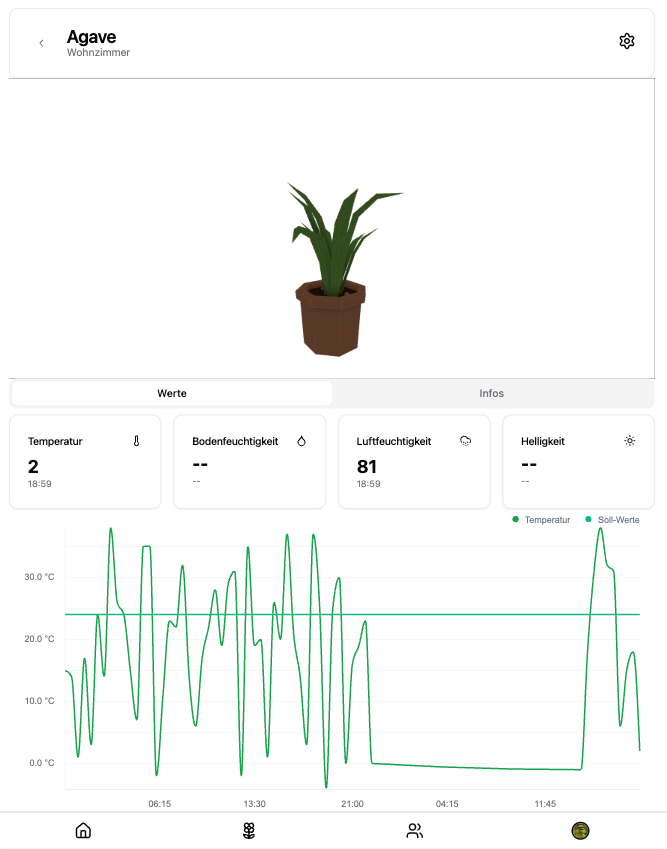
\includegraphics[scale=.5]{"./Umsetzung/images/sensora.png"}
	\caption{SinglePlantView in Aktion}
	\label{fig:SingelPlantView}
\end{figure}

Im oberen Abschnitt ist die Komponente \texttt{NavCard.vue} zu finden. Die ist für Überschriften mit einfacher Navigation zuständig in mehreren Views. Dieser Bereich ist durch die statische Anzeige des Pflanzennamens („Agave“) sowie der Rauminformation („Wohnzimmer“) gekennzeichnet. Diese Informationen werden direkt aus dem zentralen Datenmodell geladen, welches über ein Pinia-Store-Modul eingebunden ist. Der Benutzer erhält hier sofort kontextuelle Informationen zur Zuordnung der Pflanze im System.

Unmittelbar darunter befindet sich die 3D-Visualisierung der Pflanze, welche als zentrales visuelles Element prominent dargestellt ist. Diese Visualisierung basiert auf einem in der Datei \texttt{plantAvatars.ts} definierten Pflanzenmodell, das auf Basis des Pflanzentyps dynamisch geladen wird. Die Komponente zur Darstellung selbst ist als \texttt{<plant3d />} eingebettet, wobei ein Canvas-Rendering mit \texttt{Three.js} verwendet wird. Die visuelle Präsentation trägt zur Gamification der Anwendung bei, indem sie die emotionale Bindung und Wiedererkennung der Pflanzen fördern soll \cite{Werbach2012}.

Darunter folgt ein horizontal geteilter Abschnitt mit zwei Tabs: „Werte“ und „Infos“. Der Reiter „Werte“ ist standardmäßig aktiv, was sich in der visuellen Hervorhebung des Tabs zeigt. Innerhalb dieses Tabs sind vier Kartenkomponenten (Card-Komponenten) zu erkennen, die jeweils einen Umweltsensorwert repräsentieren: Temperatur, Bodenfeuchtigkeit, Luftfeuchtigkeit und Helligkeit. Diese sind als wiederverwendbare UI-Komponenten realisiert, die dynamisch Daten einlesen und anzeigen. Die Temperatur- und Luftfeuchtigkeitswerte sind im dargestellten Beispiel verfügbar („18 °C“ und „70 \%“), während Bodenfeuchte und Lichtstärke als nicht verfügbar („--“) markiert sind – ein Hinweis auf fehlerhafte oder fehlende Sensoranbindung. Jede Karte zeigt zusätzlich den letzten Messzeitpunkt, was eine präzise Einordnung der Datenqualität ermöglicht.

Der untere Teil der View wird durch die Verlaufsgraphen-Komponente dominiert, die in \texttt{PlantMeasuredValuesChart.vue} ausgelagert ist. Diese Komponente nutzt den Wrapper von \texttt{shadcn-vue} für \texttt{unovis}, um Messwerte über einen Zeitraum hinweg grafisch darzustellen. Im dargestellten Screenshot ist ein Temperaturliniendiagramm zu sehen, das über 24 Stunden  Werte anzeigt. Ein horizontaler Zielwert (Soll-Wert) ist ebenfalls dargestellt, was dem Benutzer eine sofortige Einschätzung der Umweltbedingungen erlaubt. Die Auswahl dieses Visualisierungsformats folgt dem Prinzip der kognitiven Entlastung: Durch einfache visuelle Kodierung können Zustände schneller interpretiert werden als durch numerische Tabellen.

Abgeschlossen wird die Komponente durch die \texttt{BottomNavBar.vue}, die über vier Icons eine einfache Navigation innerhalb der Anwendung ermöglicht. Diese sind als feste UI-Komponenten realisiert, wobei ein Button speziell dem Rücksprung zur Pflanzenübersicht oder der Startseite dient.

Insgesamt ergibt sich aus dieser strukturierten Aufteilung ein konsistentes, nutzerzentriertes Interface, das sowohl eine einfache Übersicht als auch eine tiefgehende Analyse einzelner Pflanzendaten erlaubt. Die klare funktionale Trennung – Datenanzeige oben, Visualisierung unten, Navigation ganz unten – folgt bewährten Usability-Prinzipien, die sich in wissenschaftlicher Literatur zur Mensch-Computer-Interaktion vielfach bewährt haben \cite{norman2013design}.



	
	\newpage

	
	% ------------- Ende Hautpteil -------------
	
	\chapter{Kritische Reflexion}
	\section{Reflexion zur Frontend-Umsetzung}

Die Umsetzung des Frontends im Rahmen dieses Projekts kann insgesamt als gelungen und stabil bewertet werden. Die Anwendung ist vollständig funktionsfähig und unterstützt sowohl die deutsche als auch die englische Sprache durch ein konsistentes Internationalisierungskonzept. Zusätzlich bietet das Interface die Auswahl zwischen einem Dark Mode und einem Light Mode, was zur Barrierefreiheit und zum Nutzungskomfort beiträgt.

Besonders hervorzuheben ist das moderne, einheitliche und visuell ansprechende Design, das konsequent auf aktuellen UI/UX-Prinzipien basiert. Durch die Integration von Gamification-Elementen wie individuellen Pflanzen-Avataren wurde die Nutzerbindung zusätzlich gestärkt. Die Verwendung bewährter Best Practices in der Frontend-Architektur sowie die Orientierung am Flux-Prinzip sorgen für einen klar strukturierten Datenfluss und eine effiziente Benutzerinteraktion.

Ein wesentlicher Aspekt der Frontend-Gestaltung war die Gewährleistung eines flüssigen Nutzererlebnisses durch intuitive Navigation und konsistente Layouts. Die modular aufgebaute Komponentenstruktur ermöglicht eine gute Wartbarkeit und einfache Erweiterbarkeit der Anwendung.

\subsection{Verbesserungspotential}

Trotz der grundsätzlich hohen Qualität bestehen einige Optimierungsmöglichkeiten. Zum einen könnten Performance-Verbesserungen vorgenommen werden, um die Ladezeiten insbesondere bei datenintensiven Ansichten zu verringern. Zum anderen wurden einige Zusatzfunktionen aus zeitlichen Gründen nicht realisiert, die in einer späteren Entwicklungsphase ergänzt werden können.

Darüber hinaus sind drei kleinere Bugs bekannt, die zum aktuellen Stand noch nicht behoben wurden:

\begin{itemize}
	\item Auf Geräten ab der Android API Version 35 kann es bei aktivierter Drei-Punkte-Navigationsleiste zu einer Überlappung mit der App-eigenen Navigationsleiste kommen.
	\item Nach der Erstellung einer neuen Gruppe werden die darin enthaltenen Räume in der Bearbeitungsansicht nicht sofort angezeigt, sofern kein Seitenwechsel oder manueller Refresh erfolgt.
    \item Man bekommt einen Fehler, wenn man eine Pflanze bearbeitet, die einen fremden Controller hat, weil im Backend diese Änderungen nicht angenommen werde.
\end{itemize}

Diese Einschränkungen haben jedoch keinen kritischen Einfluss auf die Hauptfunktionen und Nutzbarkeit der Anwendung.

Bei einer Weiter Entwicklung des Frontends und damit auch bei einer realen Nutzung sollten Frontend-Test in Verbindung mit E2E-Tests durchgeführt werden. Dadurch können Funktionen überprüft und Bugs vermieden werden. 

\subsection{Fazit}

Die in der Konzeption formulierten Anforderungen an das Frontend wurden weitestgehend erfolgreich umgesetzt. Die Anwendung bietet ein modernes, benutzerfreundliches Interface mit internationaler Ausrichtung und ansprechendem Design. Funktionalität, Nutzerfluss und Wartbarkeit konnten auf hohem Niveau realisiert werden. Die identifizierten Verbesserungspunkte bieten darüber hinaus eine wertvolle Grundlage für zukünftige Weiterentwicklungen.
	%%Reflektiere über umsetzung der Komponenten, was hat gut funktioniert, was nicht, was war einfach, was war schwer, was war unerwartet, was war nicht so gut.
\section{IoT Device}
Das IoT Device wurde von einer Person als Hauptentwickler und mehreren Unterstützenden Entwicklern erstellt.
    \subsection{Hardware}:
    Geplant war das IoT Device als ein Gerät, das die Luftfeuchtigkeit und Temperatur misst und diese Daten an einen Server sendet.
    Für die Hardware wurde ein fertiger Bausatz von Alibaba gekauft, der alle benötigten Komponenten enthielt. Damit war es möglich, die Hardware schnell zusammenzubauen und zu testen.
    Die Sensoren sind nur mittelmäßig genau, was aber für ein Proof of Concept ausreichend ist.
    \subsection{Software}:
    Die Software wurde in C entwickelt. Dabei wurde CLion mit CMake als IDE verwendet.
    Dadurch kam es zu komplikationen im Setup, da die IDE nicht richtig konfiguriert war. Daraus resultierten verzögerungen die das Projekt belasteten
    Mehr feste Entwickler hätten hier helfen können.

Insgesamt lief die Entwicklung des IoT Devices gut, aber es gab einige Herausforderungen, die bewältigt werden mussten.
    Die Hardware war einfach zusammenzubauen, aber die Software war schwieriger zu implementieren als erwartet.
    Es gab einige Probleme mit der Kommunikation zwischen dem IoT Device und dem Server, die behoben werden mussten.
    Auch die Genauigkeit der Sensoren war nicht so hoch wie erhofft, was die Ergebnisse beeinflusste.
    Dennoch konnte das IoT Device erfolgreich entwickelt und getestet werden, und es erfüllt die Anforderungen des Projekts.
    
	
	\newpage 
	
	\chapter{Ausblick}
	\section{Reflexion zur Frontend-Umsetzung}

Die Umsetzung des Frontends im Rahmen dieses Projekts kann insgesamt als gelungen und stabil bewertet werden. Die Anwendung ist vollständig funktionsfähig und unterstützt sowohl die deutsche als auch die englische Sprache durch ein konsistentes Internationalisierungskonzept. Zusätzlich bietet das Interface die Auswahl zwischen einem Dark Mode und einem Light Mode, was zur Barrierefreiheit und zum Nutzungskomfort beiträgt.

Besonders hervorzuheben ist das moderne, einheitliche und visuell ansprechende Design, das konsequent auf aktuellen UI/UX-Prinzipien basiert. Durch die Integration von Gamification-Elementen wie individuellen Pflanzen-Avataren wurde die Nutzerbindung zusätzlich gestärkt. Die Verwendung bewährter Best Practices in der Frontend-Architektur sowie die Orientierung am Flux-Prinzip sorgen für einen klar strukturierten Datenfluss und eine effiziente Benutzerinteraktion.

Ein wesentlicher Aspekt der Frontend-Gestaltung war die Gewährleistung eines flüssigen Nutzererlebnisses durch intuitive Navigation und konsistente Layouts. Die modular aufgebaute Komponentenstruktur ermöglicht eine gute Wartbarkeit und einfache Erweiterbarkeit der Anwendung.

\subsection{Verbesserungspotential}

Trotz der grundsätzlich hohen Qualität bestehen einige Optimierungsmöglichkeiten. Zum einen könnten Performance-Verbesserungen vorgenommen werden, um die Ladezeiten insbesondere bei datenintensiven Ansichten zu verringern. Zum anderen wurden einige Zusatzfunktionen aus zeitlichen Gründen nicht realisiert, die in einer späteren Entwicklungsphase ergänzt werden können.

Darüber hinaus sind drei kleinere Bugs bekannt, die zum aktuellen Stand noch nicht behoben wurden:

\begin{itemize}
	\item Auf Geräten ab der Android API Version 35 kann es bei aktivierter Drei-Punkte-Navigationsleiste zu einer Überlappung mit der App-eigenen Navigationsleiste kommen.
	\item Nach der Erstellung einer neuen Gruppe werden die darin enthaltenen Räume in der Bearbeitungsansicht nicht sofort angezeigt, sofern kein Seitenwechsel oder manueller Refresh erfolgt.
    \item Man bekommt einen Fehler, wenn man eine Pflanze bearbeitet, die einen fremden Controller hat, weil im Backend diese Änderungen nicht angenommen werde.
\end{itemize}

Diese Einschränkungen haben jedoch keinen kritischen Einfluss auf die Hauptfunktionen und Nutzbarkeit der Anwendung.

Bei einer Weiter Entwicklung des Frontends und damit auch bei einer realen Nutzung sollten Frontend-Test in Verbindung mit E2E-Tests durchgeführt werden. Dadurch können Funktionen überprüft und Bugs vermieden werden. 

\subsection{Fazit}

Die in der Konzeption formulierten Anforderungen an das Frontend wurden weitestgehend erfolgreich umgesetzt. Die Anwendung bietet ein modernes, benutzerfreundliches Interface mit internationaler Ausrichtung und ansprechendem Design. Funktionalität, Nutzerfluss und Wartbarkeit konnten auf hohem Niveau realisiert werden. Die identifizierten Verbesserungspunkte bieten darüber hinaus eine wertvolle Grundlage für zukünftige Weiterentwicklungen.
	%% Hier bisschen Tagträumen was in Zukunft noch so kommen könnte.
\section{IoT Device}
Das IoT Device könnte in Zukunft durch bessere Sensoren und eine bessere Software weiter verbessert werden.
Mehr Modularität könnte auch helfen, das IoT Device einfacher zu erweitern und anzupassen.
Das IoT Device könnte auch in Zukunft durch eine bessere Benutzeroberfläche und eine bessere Integration in andere Systeme weiter verbessert werden.
	
	\newpage
	
	%------------- Literaturverzeichnis -------------
	\newpage
	\pagestyle{fancy}
	\fancyhead[R]{LITERATUR}

	\chapter*{Literaturverzeichnis}
	\addcontentsline{toc}{chapter}{Literaturverzeichnis}
	\printbibliography
	\newpage

	%------------- Anhang -------------
	\cleardoublepage
	\fancyhead[R]{ANHANG}

	\chapter*{Anhang}
	\addcontentsline{toc}{chapter}{Anhang}

	% Hier Anhänge einfügen:
	%\input{./Anhang/sensorwerte}
	%\input{./Anhang/schaltplan}

\newpage

	
\end{document}